\section{Experiment Details and Additional Results}
\label{app:exp}

\subsection{Experiment Setting Details}
\label{app:exp_setting}

\subsubsection{Baselines}
\label{app:exp_baseline}
\begin{itemize}
    \item \textbf{Single}: A DQN or SAC learner on the target domain without any auxiliary tasks.
    \item \textbf{Auxiliary}: On the target domain, the encoder $\phi\target$ is optimized based on the loss $L_{\text{base}}(\phi\target, \pi\target) + \lambda \Big[L_P(\phi\target;\hat{P}\target)+ L_R(\phi\target;\hat{R}\target)\Big]$. Compared with our transfer algorithms which transfer the learned dynamics from source domain to the target domain, it learns the dynamics model $(\hat{P}\target, \hat{R}\target)$ on the target domain from scratch. Here we set $\lambda$ to be the same as our transferred algorithm (values of $\lambda$ are provided in Appendix~\ref{app:exp_drl}). The purpose of this baseline is to test whether the efficiency of our proposed transfer algorithms come from the transferred latent dynamics or from the auxiliary loss (or potentially both). 
    \item \textbf{Fine-tune}: To test whether our transfer algorithms benefit from loading the learned policy head $\pi\source$, on the target domain, we load the weights of $\pi\target$ from the trained source policy head $\pi\source$ and train the DQN or SAC agent without any auxiliary loss.
    \item \textbf{Time-aligned}:
    \citet{gupta2017learning} propose to learn aligned representations for two tasks, under the assumption that the source-task agent and the target-task agent reach similar latent sates at the same time step, i.e. $\phi\target(s\target_t)=\phi\source(s\source_t)$. Note that this assumption is valid when the initial state is fixed and the transitions are all deterministic. 
    Although in our setting, the agent can not learn both tasks simultaneously, we can adapt the idea of time-based alignment and encourage the target encoder to map target observations to the source representations happening at the same time step.\\
    % We adapt the idea from ~\citep{gupta2017learning} to verify that the simple alignment approach would not work in our setting. 
    % If we assume that when executing the same policy, the source and the target domain are moving forward at the same pace since they correspond to the same latent state, then we might expect the representations of source and target observations at every time step to match, i.e. $\phi\target(s\target_t)=\phi\source(s\source_t)$ at every time step $t$ when executing the same policy. 
    In our experiments, we store $N$ source trajectories $\Big\{s^{i}_0,a^{i}_0,s^{i}_{1}, a^{i}_{1},...,\Big\}_{i=1}^{N}$ collected during source task training. Then on the target domain, we first collect $N$ trajectories following the same action as the one collected from the source domain. In other words, at time step $t$ of the $i$-th trajectory, we take action $a_{t}^i$. %We cut off the target trajectory when the length of the $i$-th target trajectory becomes greater than the pre-collected $i$-th source trajectory. 
    After the target trajectories are collected, we minimize the alignment loss $L_{\text{align}}(\phi\target)=\mathbb{E}\Big[\big(\phi\target(s\target_t)-\phi\source(s\source_t)\big)^2\Big]$ to enforce that observations from source and target domain at the same time-step have the same representations.\newline
    In our experiments, we set $N$ to be 10\% of the training trajectories. (We also experimented with larger $N$', for example using all the training trajectories, but the differences are minor.) In terms the alignment loss, we optimize the loss for 1000 epochs with batch size equal to 256, where at each epoch we sample a batch of paired source and target observations and compute the alignment loss. After pre-training the target encoder, we load the weight into $\phi\target$ and resumes the normal DQN or SAC training. \\
    Our experimental results show that, although more training steps are given to the time-aligned learner, it does not outperform the single-task learner, and sometimes fails to learn (e.g. in 3DBall). The main reason is that the time-based assumption does not hold in practice as initial states are usually randomly generated. 
    Therefore, even though the agent exactly imitates the source-task policy at every step, 
    % because we cannot control the initial state distribution and the noise in each step of the transitions, we cannot expect 
    the observations from source and target task do not necessarily match at every time-step. 
    In environments with non-deterministic transitions, the state mismatch will be a more severe issue and may lead to an unreasonable encoder.
    % We implement this as a seperate baseline and empirically verify that this approach cannot improve the transfer efficiency because of the reasons we mentioned above. 
\end{itemize}

\subsubsection{Environments}
\label{app:exp_env}

\textbf{Environment Settings in Vec-to-pixel Tasks}\quad
\begin{itemize}
    \item CartPole: The source task is the same as the ordinary CartPole environment on Gym. For the pixel-input target task, we extract the screen of the environment which is of size (400,600), and crop the pixel input to let the image be centered at the cart. The resulting observation has size (40,90) after cropping. We take the difference between two consecutive frames as the agent's observation.
    \item Acrobot: The source task is the same as the ordinary Acrobot environment on Gym. For the pixel-input target task, we first extract the screen of the environment which is of size (150,150), and then down-sample the image to (40,40). We also take the difference between two consecutive frames as the agent's observation.\newline
    \item Cheetah-Run: The source task is the Cheetah Run Task provided by DeepMind Control Suite (DMC)~\citep{tassa2018deepmind}. For the target task, we use the image of size (84,84) rendered from the environment as the agent's observation.
\end{itemize}
\textbf{Environment Settings in More-sensor Tasks}\quad
For the target task of MuJoCo environments, we add the center of the mass based inertia and velocity into the observations of the agent, concatenating them with the original observation on the source task. Consequently, in the target environments, the dimensionality of the observation space on target task become much larger than that of the source task. On Hopper, the dimensionality of the target observation is 91, whereas the the source observation space only has 11 dimensions. The dimensionalities of target tasks on HalfCheetah, Hopper and Walker are 145, 91, 145 respectively.

\textbf{Environment Settings in Broken-sensor Tasks}\quad
3DBall is an example environment provided by the ML-Agents Toolkit~\citep{juliani2018unity}. In this task, the agent (a cube) is supposed to balance a ball on its top. At every step, the agent will be rewarded if the ball is still on its top. If the ball falls off, the episode will immediately end.
The highest episodic return in this task is 100. 
There are two versions of this game, which only differ by their observation spaces.
The simpler version (named 3DBall in the toolkit) has 8 observation features corresponding to the rotation of the agent cube, and the position and velocity of the ball.
The harder version (named 3DBallHard in the toolkit) does not have access to the ball velocity, but observes a stack of 9 past frames, each of which corresponds to the rotation of the agent cube, and the position of the ball, resulting in 45 observation dimensions at every step.
We regard 3DBall as the source task and 3DBallHard as the target task in our experiments.

\subsubsection{Implementation of Base DRL Algorithms and Hyper-parameter Settings}
\label{app:exp_drl}

\textbf{Implementation of DQN}\quad
To ensure that the base learning algorithm learns the pixel-input target tasks well, we follow the existing online codebases for pre-processing, architectures and hyperparameter settings in pixel CartPole\footnote{\href{https://pytorch.org/tutorials/intermediate/reinforcement_q_learning.html}{https://pytorch.org/tutorials/intermediate/reinforcement\_q\_learning.html}} and pixel Acrobot
% we follow the pre-processing, architectures, and hyperparameters from another codebase 
\footnote{\href{https://github.com/eyalbd2/Deep_RL_Course }{https://github.com\/eyalbd2\/Deep\_RL\_Course}}. On source domain, the DQN network has a 2-layer encoder and a 2-layer Q head of hidden size 64, and the representation dimension is set as 16. For pixel-input, the encoder has three convolution layers followed by a linear layer. The number of channels of the convolutional layers are equal to 16, 32, 32, respectively (kernel size=5 for all three layers). We use the Adam optimizer with learning rate $0.001$ and $\beta_1, \beta_2=0.9,0.999$. The target Q network is updated every 10 iterations.
% We let the dynamics models $\apa$ and $\ara$ be linear, so that the representation be more informative in terms of representing the transition dynamics.
In CartPole, we use a replay buffer with size 10000. In the more challenging Acrobot, we use a prioritized replay buffer with size 100000.
%\ys{Ruijie: can you put more details here? including hyperparameters, as in the %rebuttal}

\textbf{Implementation of SAC}\quad
% We conduct the experiments of transfer SAC on MuJoCo-v3 using TITAN RTX GPU.
For MuJoCo environments, we follow an elegant open-sourced SAC implementation\footnote{\href{https://github.com/pranz24/pytorch-soft-actor-critic}{https://github.com/pranz24/pytorch-soft-actor-critic}}.
The number of hidden units for all neural networks is 256.
The actor has a two-layer encoder and a two-layer policy head.
The two Q networks both have three linear layers.
The activation function is ReLU and the learning rate is $3\cdot 10^{-4}$.
% The regularization weight is set as 1.
We train the dynamics model and the reward model every 50k interactive steps in the source task.
For the DMC environment Cheetah-Run, we follow the open-sourced SAC implementation with an autoencoder \footnote{\href{https://github.com/denisyarats/pytorch_sac_ae}{https://github.com/denisyarats/pytorch\_sac\_ae}}.
The pixel encoder has three convolution layers and one linear layer. The number of channels for all convolutional layers is 32 and the kernel size is 3.
For the 3DBall environment, as it can only be learned within the ML-Agents toolkit, we directly use the SAC implementation provided by the toolkit with the default hyperparameter settings. 


\textbf{Implementation of Latent Dynamics Model}\quad
Note that our goal is to learn a good representation by enforcing it predicting the latent dynamics, different from model-based RL~\citep{hafner2019dream} that aims to learn accurate models for planning. Therefore, we let the dynamics models $\hat{P}$ and $\hat{R}$ be simple linear networks, so that the representation can be more informative in terms of representing dynamics and learning values/policies. For environments with discrete action spaces, we learn $|\actions|$ linear transition networks and $|\actions|$ linear reward models. For environments with continuous action spaces, we first learn an action encoder $\psi: \actions \to \mathbb{R}^d$ with the same encoding size $d$ as the state representation. Then, we learn a linear transition network and a linear reward network with $\hat{P}(\phi(o)\circ\psi(a))$ being the predicted next representation, and $\hat{R}(\phi(o)\circ\psi(a))$ being the predicted reward, where $\circ$ denotes element-wise product. In practice, we find this implementation achieves good performance across many environments. \\
In addition, note that due to the significant difference between source observation and target observation, the initial encoding scale could be very different in source and target tasks, making it hard for them to be regularized by the same dynamics model. Therefore, we normalize the output of both encoders to be a unit vector (l2 norm is 1), which remedies the potential mismatch in their scales.

\textbf{Hyperparameter Settings for Transfer Learning}\quad
In experiments, we find that it is better to set $\lambda$ relatively large when the environment dynamics are simple and the dynamics model is of high quality. When the environment dynamics is complex, we choose to be more conservative and set $\lambda$ to be smaller. Concretely, in CartPole, $\lambda$ is set as 18; in 3DBall, $\lambda$ is set as 10; in Acrobot, $\lambda$ is set as 5; in the remaining MuJoCo environments where dynamics are more complicated, $\lambda$ is set as 1. Although we use different $\lambda$'s in different environments based on domain knowledge, we find that different values of $\lambda$'s do not have much influence on the learning performance. Figure~\ref{fig:hyper} provided in Appendix~\ref{app:exp_results} shows a test on the hyper-parameter $\lambda$, where we can see that our algorithm effectively transfers knowledge under various values of $\lambda$. \\
Regarding the representation dimension, we set it to be smaller for simpler tasks, and larger for more complex tasks. In 3DBall, we set the encoding size to be 8; in CartPole, we set the encoding size as 16; in Acrobot, we set the encoding size as 32; in Cheetah-Run, we set the encoding size as 50; in MuJoCo tasks, we set the encoding size as 256. Again, we find that the feature size does not influence the performance too much. But based on the theoretical insights of learning minimal sufficient representation~\cite{achille2018emergence}, we believe that it is generally better to have a lower-dimensional representation while making sure it is sufficient for learning.

\newpage 
\subsection{Additional Experimental Results}
\label{app:exp_results}

\textbf{Ablation Study: Transferring Different Components}\\
Figure~\ref{fig:mujoco_ablation} shows the ablation study of our method in continuous control tasks. We compare our method with the following variants:\\
(1) learning auxiliary tasks without transfer, \\
(2) only transferring transition models $\hat{P}$ and \\
(3) only transferring reward models $\hat{R}$.

Compared with the single-task learning baseline (the blue curves), we find that all the variants of our method can make some improvements, which suggests that learning dynamics models as auxiliary tasks, transferring $\hat{P}$ and $\hat{R}$ are all effective designs for accelerating the target task learning. Finally, our method (the red curves) that combines the above components achieves the best performance, justifying the effectiveness of our transfer algorithm.


\begin{figure}[!htbp]
\centering
 \begin{subfigure}[t]{0.48\columnwidth}
  \centering
  % This file was created with tikzplotlib v0.9.12.
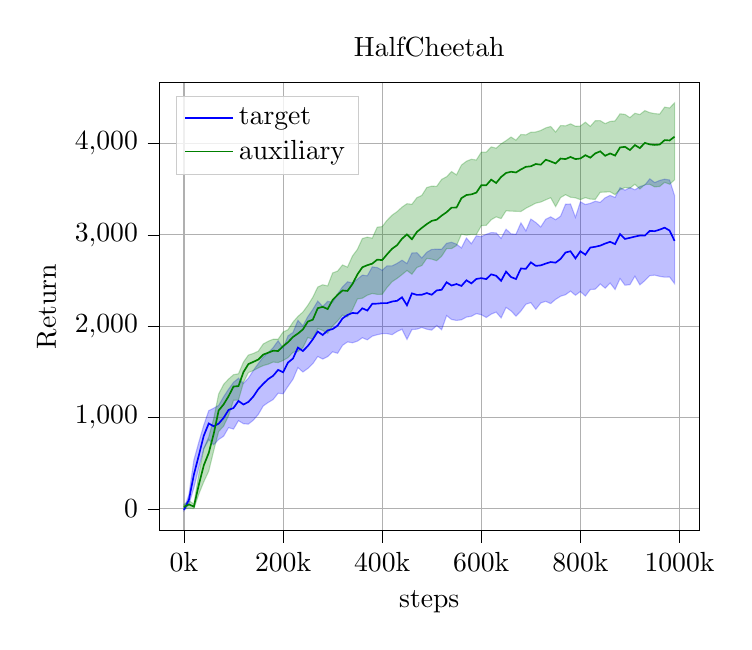
\begin{tikzpicture}

\begin{axis}[
legend cell align={left},
legend style={
  fill opacity=0.8,
  draw opacity=1,
  text opacity=1,
  at={(0.03,0.97)},
  anchor=north west,
  draw=white!80!black
},
tick align=outside,
tick pos=left,
title={HalfCheetah},
x grid style={white!69.0196078431373!black},
xlabel={steps},
xmajorgrids,
xmin=-4.95, xmax=103.95,
xtick style={color=black},
xtick={0,20,40,60,80,100},
xticklabels={0k,200k,400k,600k,800k,1000k},
y grid style={white!69.0196078431373!black},
ylabel={Return},
ymajorgrids,
ymin=-240.674849660313, ymax=4667.87126650874,
ytick style={color=black}
]
\path [draw=blue, fill=blue, opacity=0.25]
(axis cs:0,-4.86148704856668)
--(axis cs:0,-17.5591171071745)
--(axis cs:1,51.1807257704293)
--(axis cs:2,229.478935904115)
--(axis cs:3,448.93792198758)
--(axis cs:4,657.525204760701)
--(axis cs:5,757.207708252639)
--(axis cs:6,701.869778418762)
--(axis cs:7,759.366205411334)
--(axis cs:8,795.083782295168)
--(axis cs:9,888.796808502576)
--(axis cs:10,873.303965999891)
--(axis cs:11,965.748649024855)
--(axis cs:12,932.145979641106)
--(axis cs:13,927.466093586972)
--(axis cs:14,971.046906932384)
--(axis cs:15,1033.46308367243)
--(axis cs:16,1126.23850912815)
--(axis cs:17,1164.34520949092)
--(axis cs:18,1196.43983301424)
--(axis cs:19,1265.79933943031)
--(axis cs:20,1259.71535664198)
--(axis cs:21,1341.23107583601)
--(axis cs:22,1418.50650749061)
--(axis cs:23,1546.69437012274)
--(axis cs:24,1498.12664853701)
--(axis cs:25,1537.21567787302)
--(axis cs:26,1589.3980625322)
--(axis cs:27,1667.97544158709)
--(axis cs:28,1639.94660937953)
--(axis cs:29,1666.97281766284)
--(axis cs:30,1719.14397346101)
--(axis cs:31,1702.56248560516)
--(axis cs:32,1789.46028337378)
--(axis cs:33,1827.50605094207)
--(axis cs:34,1818.18539735303)
--(axis cs:35,1835.37310504401)
--(axis cs:36,1873.14717246469)
--(axis cs:37,1850.21121090857)
--(axis cs:38,1890.80118715084)
--(axis cs:39,1906.1778271455)
--(axis cs:40,1917.81410125555)
--(axis cs:41,1918.27077471886)
--(axis cs:42,1906.90951395059)
--(axis cs:43,1940.9378802823)
--(axis cs:44,1966.49550484835)
--(axis cs:45,1855.21963803132)
--(axis cs:46,1962.70875161607)
--(axis cs:47,1967.17871312954)
--(axis cs:48,1985.80208675596)
--(axis cs:49,1966.70145832544)
--(axis cs:50,1956.31438170074)
--(axis cs:51,2007.40005485832)
--(axis cs:52,1960.94457203168)
--(axis cs:53,2115.76406628063)
--(axis cs:54,2073.14380478075)
--(axis cs:55,2062.73894867009)
--(axis cs:56,2069.68845920919)
--(axis cs:57,2099.27344654391)
--(axis cs:58,2108.23750765726)
--(axis cs:59,2137.53995349505)
--(axis cs:60,2125.28148950372)
--(axis cs:61,2095.50566468756)
--(axis cs:62,2131.85670650373)
--(axis cs:63,2154.08177409947)
--(axis cs:64,2090.4217368938)
--(axis cs:65,2205.56467756056)
--(axis cs:66,2167.37700874322)
--(axis cs:67,2110.42398533225)
--(axis cs:68,2165.6675132361)
--(axis cs:69,2239.90314905439)
--(axis cs:70,2257.45096951806)
--(axis cs:71,2184.80701985497)
--(axis cs:72,2253.61589662606)
--(axis cs:73,2271.75713675878)
--(axis cs:74,2247.44848749397)
--(axis cs:75,2293.38808919841)
--(axis cs:76,2327.3338124809)
--(axis cs:77,2344.50823743256)
--(axis cs:78,2383.46044865038)
--(axis cs:79,2338.58097866277)
--(axis cs:80,2378.77371255312)
--(axis cs:81,2329.94024828125)
--(axis cs:82,2401.21599876009)
--(axis cs:83,2404.93176530972)
--(axis cs:84,2462.09922111143)
--(axis cs:85,2416.58321139241)
--(axis cs:86,2472.18820156346)
--(axis cs:87,2401.75734499535)
--(axis cs:88,2521.78214117514)
--(axis cs:89,2448.4385863152)
--(axis cs:90,2454.36633291909)
--(axis cs:91,2547.48116026531)
--(axis cs:92,2452.19452140337)
--(axis cs:93,2498.5337474189)
--(axis cs:94,2553.05102193357)
--(axis cs:95,2558.58855809078)
--(axis cs:96,2545.24526888484)
--(axis cs:97,2536.47260310106)
--(axis cs:98,2538.69264305889)
--(axis cs:99,2466.10031442603)
--(axis cs:99,3429.73633614058)
--(axis cs:99,3429.73633614058)
--(axis cs:98,3600.19483203576)
--(axis cs:97,3609.05898310111)
--(axis cs:96,3595.56040284393)
--(axis cs:95,3572.28024972714)
--(axis cs:94,3613.24166875524)
--(axis cs:93,3544.66762501971)
--(axis cs:92,3528.62248720776)
--(axis cs:91,3492.78707671457)
--(axis cs:90,3517.667690518)
--(axis cs:89,3488.36895708831)
--(axis cs:88,3515.97021563052)
--(axis cs:87,3408.86697033635)
--(axis cs:86,3431.67246057134)
--(axis cs:85,3405.30515463493)
--(axis cs:84,3355.36328210851)
--(axis cs:83,3367.5712022178)
--(axis cs:82,3344.26577317076)
--(axis cs:81,3331.87986626372)
--(axis cs:80,3360.95944769142)
--(axis cs:79,3192.03867513452)
--(axis cs:78,3337.41284049053)
--(axis cs:77,3334.67930968438)
--(axis cs:76,3203.52318082358)
--(axis cs:75,3165.48306262993)
--(axis cs:74,3196.9657868547)
--(axis cs:73,3170.37831381546)
--(axis cs:72,3085.88128515625)
--(axis cs:71,3135.26280986177)
--(axis cs:70,3172.04581537129)
--(axis cs:69,3042.49156585731)
--(axis cs:68,3130.95983024521)
--(axis cs:67,3006.23351914661)
--(axis cs:66,3010.36084991637)
--(axis cs:65,3061.96904802812)
--(axis cs:64,2960.86823235794)
--(axis cs:63,3021.00020237101)
--(axis cs:62,3024.30063303229)
--(axis cs:61,3006.1056918483)
--(axis cs:60,2979.47533509475)
--(axis cs:59,2989.14048143868)
--(axis cs:58,2902.36073242958)
--(axis cs:57,2964.00134115517)
--(axis cs:56,2856.08535549337)
--(axis cs:55,2897.64980906998)
--(axis cs:54,2918.53210815763)
--(axis cs:53,2907.1098009003)
--(axis cs:52,2841.92852717021)
--(axis cs:51,2842.81428213655)
--(axis cs:50,2840.14069204298)
--(axis cs:49,2809.02737598103)
--(axis cs:48,2746.34388983844)
--(axis cs:47,2803.95951577019)
--(axis cs:46,2800.78461369805)
--(axis cs:45,2685.20930384405)
--(axis cs:44,2722.30905640814)
--(axis cs:43,2686.57615406201)
--(axis cs:42,2659.9353500308)
--(axis cs:41,2660.46619329571)
--(axis cs:40,2611.91254176405)
--(axis cs:39,2641.52294218534)
--(axis cs:38,2648.59991959234)
--(axis cs:37,2551.10348217818)
--(axis cs:36,2558.98761300813)
--(axis cs:35,2513.87523127286)
--(axis cs:34,2472.57193422726)
--(axis cs:33,2485.78011361719)
--(axis cs:32,2430.33583935113)
--(axis cs:31,2351.62944426776)
--(axis cs:30,2260.16818253518)
--(axis cs:29,2271.80487765026)
--(axis cs:28,2216.17344222787)
--(axis cs:27,2274.73924856425)
--(axis cs:26,2182.78462728207)
--(axis cs:25,2105.03297091567)
--(axis cs:24,2002.76471098274)
--(axis cs:23,2063.81917319444)
--(axis cs:22,1931.4797890585)
--(axis cs:21,1893.3911672037)
--(axis cs:20,1759.62364531051)
--(axis cs:19,1840.82107672777)
--(axis cs:18,1765.11613068137)
--(axis cs:17,1708.06697480238)
--(axis cs:16,1662.18933618276)
--(axis cs:15,1590.71041692961)
--(axis cs:14,1515.01317841607)
--(axis cs:13,1430.18553005668)
--(axis cs:12,1372.34166219899)
--(axis cs:11,1429.94729091468)
--(axis cs:10,1384.97568876844)
--(axis cs:9,1309.70085830112)
--(axis cs:8,1226.24186587736)
--(axis cs:7,1132.24292067991)
--(axis cs:6,1102.01694138893)
--(axis cs:5,1074.31466392856)
--(axis cs:4,916.552807066411)
--(axis cs:3,729.373016177397)
--(axis cs:2,532.826825376399)
--(axis cs:1,155.669164879405)
--(axis cs:0,-4.86148704856668)
--cycle;

\path [draw=green!50.1960784313725!black, fill=green!50.1960784313725!black, opacity=0.25]
(axis cs:0,47.2047364255923)
--(axis cs:0,-2.65915644867213)
--(axis cs:1,7.51692988665886)
--(axis cs:2,2.38678973627775)
--(axis cs:3,160.713235021052)
--(axis cs:4,296.105999231114)
--(axis cs:5,412.613442177057)
--(axis cs:6,635.412151240929)
--(axis cs:7,847.031035859417)
--(axis cs:8,905.028610959436)
--(axis cs:9,1019.60461168053)
--(axis cs:10,1188.82108857787)
--(axis cs:11,1190.5085194263)
--(axis cs:12,1382.01572626336)
--(axis cs:13,1491.57408048096)
--(axis cs:14,1513.47939710068)
--(axis cs:15,1543.45539216917)
--(axis cs:16,1568.19165295542)
--(axis cs:17,1583.58613897989)
--(axis cs:18,1607.24387426497)
--(axis cs:19,1601.47233951863)
--(axis cs:20,1623.91883274357)
--(axis cs:21,1655.58702557294)
--(axis cs:22,1713.14309917408)
--(axis cs:23,1723.00301876539)
--(axis cs:24,1764.2096155033)
--(axis cs:25,1876.27438065925)
--(axis cs:26,1857.38824665802)
--(axis cs:27,1974.19610216807)
--(axis cs:28,1952.79070648111)
--(axis cs:29,1921.82042515931)
--(axis cs:30,2002.68321365198)
--(axis cs:31,2057.12251435356)
--(axis cs:32,2121.2093685317)
--(axis cs:33,2101.51759483253)
--(axis cs:34,2179.74512110872)
--(axis cs:35,2297.12600263884)
--(axis cs:36,2306.09183625888)
--(axis cs:37,2339.26064838504)
--(axis cs:38,2357.88333149311)
--(axis cs:39,2348.2997038981)
--(axis cs:40,2349.0747641075)
--(axis cs:41,2424.91556352374)
--(axis cs:42,2486.51169869601)
--(axis cs:43,2522.50526384538)
--(axis cs:44,2563.92261255278)
--(axis cs:45,2609.93007796049)
--(axis cs:46,2568.86027387872)
--(axis cs:47,2641.7959794716)
--(axis cs:48,2663.95433365989)
--(axis cs:49,2741.77496274705)
--(axis cs:50,2733.54374393341)
--(axis cs:51,2716.7273530754)
--(axis cs:52,2765.71454855578)
--(axis cs:53,2848.58810800324)
--(axis cs:54,2849.02752974287)
--(axis cs:55,2882.70700759689)
--(axis cs:56,3007.53995641982)
--(axis cs:57,2996.56017294282)
--(axis cs:58,3004.21225172137)
--(axis cs:59,3003.51733438876)
--(axis cs:60,3099.9347871723)
--(axis cs:61,3104.36958824834)
--(axis cs:62,3165.31179122242)
--(axis cs:63,3196.55342107074)
--(axis cs:64,3178.13704473715)
--(axis cs:65,3263.20271116445)
--(axis cs:66,3259.47401928986)
--(axis cs:67,3257.67719428826)
--(axis cs:68,3255.20514369804)
--(axis cs:69,3290.55974069051)
--(axis cs:70,3318.05896426068)
--(axis cs:71,3346.87064735074)
--(axis cs:72,3358.80013395085)
--(axis cs:73,3383.0300246677)
--(axis cs:74,3406.34251788852)
--(axis cs:75,3309.32513269053)
--(axis cs:76,3407.78613484326)
--(axis cs:77,3439.69492349899)
--(axis cs:78,3411.69985102143)
--(axis cs:79,3405.34183770809)
--(axis cs:80,3385.18551455515)
--(axis cs:81,3407.45635642855)
--(axis cs:82,3390.90773071852)
--(axis cs:83,3388.7050421717)
--(axis cs:84,3465.56636104986)
--(axis cs:85,3468.74785503741)
--(axis cs:86,3471.03384836968)
--(axis cs:87,3439.5383167058)
--(axis cs:88,3494.32319277098)
--(axis cs:89,3518.10636253971)
--(axis cs:90,3510.30273783052)
--(axis cs:91,3554.15917551649)
--(axis cs:92,3501.9608051066)
--(axis cs:93,3550.49597652156)
--(axis cs:94,3553.35712414308)
--(axis cs:95,3524.63508828543)
--(axis cs:96,3529.54277285338)
--(axis cs:97,3574.44508569631)
--(axis cs:98,3554.03049375633)
--(axis cs:99,3601.72846493995)
--(axis cs:99,4444.7555339556)
--(axis cs:99,4444.7555339556)
--(axis cs:98,4388.85883828941)
--(axis cs:97,4398.18153950046)
--(axis cs:96,4321.9731418338)
--(axis cs:95,4327.18930208247)
--(axis cs:94,4337.85993818148)
--(axis cs:93,4359.95787748152)
--(axis cs:92,4316.80835324122)
--(axis cs:91,4331.00902272161)
--(axis cs:90,4282.89867144423)
--(axis cs:89,4318.48839157845)
--(axis cs:88,4324.8436637386)
--(axis cs:87,4246.9359584758)
--(axis cs:86,4241.54341226975)
--(axis cs:85,4217.30402327563)
--(axis cs:84,4249.89359660185)
--(axis cs:83,4249.25248994419)
--(axis cs:82,4187.78229665748)
--(axis cs:81,4233.12465924577)
--(axis cs:80,4190.89527432862)
--(axis cs:79,4188.40795429288)
--(axis cs:78,4214.92979123969)
--(axis cs:77,4193.10842817833)
--(axis cs:76,4196.41483465942)
--(axis cs:75,4125.30822629123)
--(axis cs:74,4186.12066194708)
--(axis cs:73,4170.77776927206)
--(axis cs:72,4142.73417961138)
--(axis cs:71,4125.69964662831)
--(axis cs:70,4123.43803207798)
--(axis cs:69,4094.48675837182)
--(axis cs:68,4098.49135866485)
--(axis cs:67,4036.19174129836)
--(axis cs:66,4070.43356129305)
--(axis cs:65,4031.24329725839)
--(axis cs:64,3996.37822690603)
--(axis cs:63,3948.53368041693)
--(axis cs:62,3962.82804552951)
--(axis cs:61,3905.54735504158)
--(axis cs:60,3905.15212009017)
--(axis cs:59,3818.92804370427)
--(axis cs:58,3827.40755069082)
--(axis cs:57,3805.51291343862)
--(axis cs:56,3763.7490395991)
--(axis cs:55,3656.63062612847)
--(axis cs:54,3692.32688159955)
--(axis cs:53,3635.82299621915)
--(axis cs:52,3607.03792786311)
--(axis cs:51,3530.21755246871)
--(axis cs:50,3532.97674798691)
--(axis cs:49,3517.82473109009)
--(axis cs:48,3431.58852723932)
--(axis cs:47,3405.71650242836)
--(axis cs:46,3333.95638343952)
--(axis cs:45,3340.65732373052)
--(axis cs:44,3302.96718256399)
--(axis cs:43,3253.40102121344)
--(axis cs:42,3215.36042123354)
--(axis cs:41,3160.6520723303)
--(axis cs:40,3089.64384971076)
--(axis cs:39,3083.60112429254)
--(axis cs:38,2963.38567360397)
--(axis cs:37,2974.43495463525)
--(axis cs:36,2959.4095146885)
--(axis cs:35,2840.29437689475)
--(axis cs:34,2768.00431648625)
--(axis cs:33,2646.73601122411)
--(axis cs:32,2669.66266133294)
--(axis cs:31,2603.51594463333)
--(axis cs:30,2582.17809220897)
--(axis cs:29,2440.71533650271)
--(axis cs:28,2453.08094837111)
--(axis cs:27,2428.48771622382)
--(axis cs:26,2316.0640376844)
--(axis cs:25,2228.76974982929)
--(axis cs:24,2154.63570934645)
--(axis cs:23,2106.48822784136)
--(axis cs:22,2044.14205864596)
--(axis cs:21,1961.37307447775)
--(axis cs:20,1935.27033802111)
--(axis cs:19,1857.02174332084)
--(axis cs:18,1856.89258792916)
--(axis cs:17,1834.68195819241)
--(axis cs:16,1804.73038547795)
--(axis cs:15,1726.34256646555)
--(axis cs:14,1701.21377905242)
--(axis cs:13,1683.5305610349)
--(axis cs:12,1606.46156900964)
--(axis cs:11,1478.75889326971)
--(axis cs:10,1468.43846645296)
--(axis cs:9,1420.37085666422)
--(axis cs:8,1361.94347139281)
--(axis cs:7,1256.52586651271)
--(axis cs:6,987.467237824806)
--(axis cs:5,787.77945201487)
--(axis cs:4,660.78866232566)
--(axis cs:3,379.112584179643)
--(axis cs:2,52.3205714661793)
--(axis cs:1,89.3517280243388)
--(axis cs:0,47.2047364255923)
--cycle;

\addplot [semithick, blue]
table {%
0 -11.0178532331251
1 99.3175684184132
2 374.967228209651
3 585.090791596031
4 800.964306939033
5 934.525211183715
6 904.041870461718
7 932.526515873367
8 995.951482366304
9 1082.78017530664
10 1103.71862766219
11 1181.23448416646
12 1142.21670535143
13 1169.93760012654
14 1229.4609466636
15 1310.15105565182
16 1368.76614089292
17 1420.58888886806
18 1457.14276829857
19 1521.23007808936
20 1495.37800553284
21 1601.65954950899
22 1645.6470738063
23 1765.62094669983
24 1727.49279773991
25 1783.81909939981
26 1855.4503665983
27 1940.93592472679
28 1903.23239254481
29 1953.4588967603
30 1968.40063838392
31 2005.37694142948
32 2084.83037912967
33 2122.25438575824
34 2144.89859063938
35 2139.58945512007
36 2195.76515955755
37 2170.87472495984
38 2244.59102596719
39 2246.57750872989
40 2252.31598304335
41 2252.28724483783
42 2269.56049158407
43 2277.501825042
44 2316.17536571358
45 2228.7366525669
46 2359.13475520781
47 2342.27628201564
48 2344.22458243234
49 2362.62794434487
50 2344.08638351857
51 2391.18394357459
52 2398.56698372182
53 2480.62196549585
54 2445.04571237694
55 2461.2332691673
56 2440.47915931298
57 2502.26540589374
58 2468.53726169202
59 2516.5536106501
60 2525.73976777404
61 2515.37603606665
62 2566.9845403377
63 2551.93125426656
64 2496.82884571014
65 2597.01541495871
66 2537.97934238333
67 2515.8433879843
68 2631.51043121734
69 2627.83115340806
70 2698.50343368259
71 2660.21187632907
72 2665.62705678322
73 2684.98678718212
74 2702.12728072576
75 2695.26456800156
76 2736.27364572059
77 2806.457254686
78 2819.9594786753
79 2742.04967054093
80 2820.02374862494
81 2782.82777189531
82 2860.59167998306
83 2869.17329115044
84 2881.60968539021
85 2904.54788711714
86 2923.69018177732
87 2898.37483159722
88 3008.2075991589
89 2954.90484072822
90 2967.36182706912
91 2980.68918697353
92 2992.36963770973
93 2991.38658228289
94 3043.22934612388
95 3039.96004102946
96 3057.00328221454
97 3078.29853296243
98 3046.86848749743
99 2933.98292394914
};
\addlegendentry{target}
\addplot [semithick, green!50.1960784313725!black]
table {%
0 20.5696111612188
1 48.0113643633792
2 23.9326775645735
3 263.420325934951
4 476.027106488257
5 612.091855565621
6 820.264622963629
7 1076.88527759144
8 1143.11165119737
9 1233.0145525565
10 1338.98363757531
11 1343.54246053364
12 1496.68721226347
13 1584.69030107945
14 1609.07812145909
15 1634.42024212684
16 1688.4847478774
17 1709.53258183138
18 1731.02642002858
19 1728.04305525034
20 1780.68481271617
21 1823.87809333996
22 1881.86067223376
23 1918.84797041333
24 1963.82643941022
25 2050.48796699402
26 2070.58813965536
27 2196.55811221607
28 2211.61733189153
29 2187.3314845781
30 2286.4771330027
31 2343.25612995444
32 2390.5108346818
33 2385.74250485813
34 2461.21164987108
35 2566.39039359839
36 2644.75436882838
37 2667.56233731144
38 2684.52466292662
39 2728.53203686652
40 2723.13923526562
41 2787.45771765632
42 2847.64900083437
43 2886.26836516029
44 2957.07571877131
45 3004.70288232187
46 2951.65883856072
47 3031.24453900284
48 3076.07046593034
49 3117.23444074912
50 3152.695293649
51 3165.83898937797
52 3210.06977101411
53 3247.90044888395
54 3297.60036487645
55 3298.73714352346
56 3401.72861330504
57 3435.64557713235
58 3443.08621399967
59 3461.86352476213
60 3542.15915658113
61 3542.18600929014
62 3603.97529191755
63 3567.42897644656
64 3633.22451386287
65 3677.54323666284
66 3690.39776615333
67 3682.89594005184
68 3716.38003739321
69 3744.67692846559
70 3750.47809950442
71 3775.26637933617
72 3767.86672666008
73 3821.82163828324
74 3803.57926696622
75 3781.89095621824
76 3835.23769932098
77 3829.24022207784
78 3852.49464263772
79 3829.21268146349
80 3835.85044645023
81 3871.99406468128
82 3844.57924318378
83 3891.61620582388
84 3914.02310593033
85 3865.61338159537
86 3891.06175114807
87 3867.60495005668
88 3956.81581728201
89 3963.47438359381
90 3928.32375148463
91 3982.54623064233
92 3949.4440846463
93 4006.60381573548
94 3990.05268659494
95 3984.19223474651
96 3988.524651105
97 4037.14704255342
98 4033.24808371652
99 4074.3076922873
};
\addlegendentry{auxiliary}
\end{axis}

\end{tikzpicture}

 \end{subfigure}
 \hfill
 \hspace{-1em}
 \begin{subfigure}[t]{0.48\columnwidth}
  \centering
  % This file was created with tikzplotlib v0.9.12.
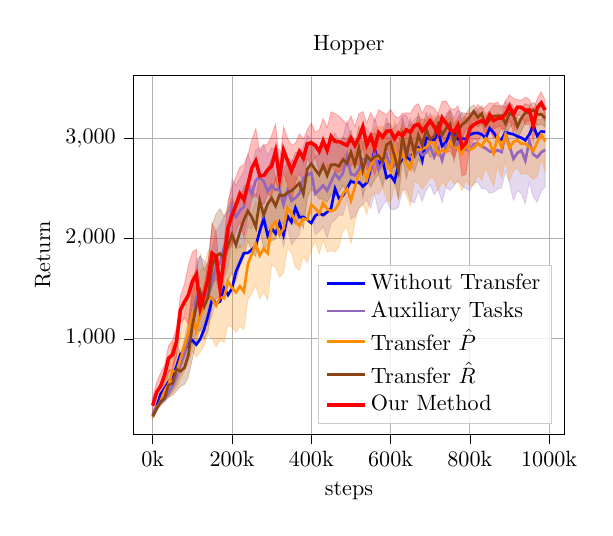
\begin{tikzpicture}[scale=0.8]

\definecolor{color0}{rgb}{1,0.549019607843137,0}
% \definecolor{color1}{rgb}{0.501960784313725,0,0.501960784313725}
% \definecolor{color1}{rgb}{0.4,0.69803921568,1}
\definecolor{color1}{rgb}{0.55,0.27,0.07}
\definecolor{color2}{rgb}{0.580392156862745,0.403921568627451,0.741176470588235}
\begin{axis}[
legend cell align={left},
legend style={
  fill opacity=0.8,
  draw opacity=1,
  text opacity=1,
  at={(0.97,0.03)},
  anchor=south east,
  draw=white!80!black
},
tick align=outside,
tick pos=left,
title={{Hopper}},
x grid style={white!69.0196078431373!black},
xlabel={{steps}},
xmajorgrids,
xmin=-4.95, xmax=103.95,
xtick style={color=black},
xtick={0,20,40,60,80,100},
xticklabels={0k,200k,400k,600k,800k,1000k},
y grid style={white!69.0196078431373!black},
ymajorgrids,
ylabel={{Return}},
ymin=47.2517038881593, ymax=3624.97592162401,
ytick style={color=black}
]



\path [draw=color2, fill=color2, opacity=0.25]
(axis cs:0,247.292806366722)
--(axis cs:0,221.85711389826)
--(axis cs:1,309.783743040074)
--(axis cs:2,344.728043361613)
--(axis cs:3,375.024082998293)
--(axis cs:4,416.396594859147)
--(axis cs:5,476.350161093595)
--(axis cs:6,548.190779644293)
--(axis cs:7,639.852004069495)
--(axis cs:8,705.470059994717)
--(axis cs:9,830.689557495225)
--(axis cs:10,925.030610410932)
--(axis cs:11,1067.63688543197)
--(axis cs:12,1085.52278400633)
--(axis cs:13,1133.09061679767)
--(axis cs:14,1143.7796502912)
--(axis cs:15,1229.51500162515)
--(axis cs:16,1400.26966379336)
--(axis cs:17,1371.05936692635)
--(axis cs:18,1607.01540508912)
--(axis cs:19,1706.93285070991)
--(axis cs:20,1986.5199169859)
--(axis cs:21,1899.57222798881)
--(axis cs:22,1908.12267972762)
--(axis cs:23,1932.24488922602)
--(axis cs:24,2117.08583199424)
--(axis cs:25,2093.02468017649)
--(axis cs:26,2216.69322470528)
--(axis cs:27,2255.9492834924)
--(axis cs:28,2143.50203009065)
--(axis cs:29,2094.98168285379)
--(axis cs:30,2123.79485136005)
--(axis cs:31,2051.47663367561)
--(axis cs:32,2090.39942794534)
--(axis cs:33,1916.07755622759)
--(axis cs:34,2114.62697693972)
--(axis cs:35,1936.78324889936)
--(axis cs:36,1991.33529915474)
--(axis cs:37,2037.11745190284)
--(axis cs:38,2234.48594650153)
--(axis cs:39,2194.65806945007)
--(axis cs:40,2253.53260710441)
--(axis cs:41,2035.23334889978)
--(axis cs:42,2071.49846847513)
--(axis cs:43,2114.55817666617)
--(axis cs:44,2006.08629906251)
--(axis cs:45,2152.45555530958)
--(axis cs:46,2189.03297283975)
--(axis cs:47,2232.4872949305)
--(axis cs:48,2230.63955101515)
--(axis cs:49,2388.64946213562)
--(axis cs:50,2192.24747896927)
--(axis cs:51,2221.49765687323)
--(axis cs:52,2300.10721649776)
--(axis cs:53,2341.27918173073)
--(axis cs:54,2386.20026295494)
--(axis cs:55,2301.95393605178)
--(axis cs:56,2447.90496139067)
--(axis cs:57,2246.22990420658)
--(axis cs:58,2329.38797717438)
--(axis cs:59,2378.93916745534)
--(axis cs:60,2291.21622953324)
--(axis cs:61,2288.8515543347)
--(axis cs:62,2312.33428378439)
--(axis cs:63,2484.82778342949)
--(axis cs:64,2492.87674797247)
--(axis cs:65,2376.76478960012)
--(axis cs:66,2354.77818568314)
--(axis cs:67,2471.43198310546)
--(axis cs:68,2371.19023052219)
--(axis cs:69,2485.49989605906)
--(axis cs:70,2535.74813095094)
--(axis cs:71,2436.87887940527)
--(axis cs:72,2490.0651220222)
--(axis cs:73,2360.90722307716)
--(axis cs:74,2513.21546987917)
--(axis cs:75,2481.17416626682)
--(axis cs:76,2524.56442386035)
--(axis cs:77,2580.72822291951)
--(axis cs:78,2525.88989491583)
--(axis cs:79,2497.77395792081)
--(axis cs:80,2480.69732614854)
--(axis cs:81,2553.76770368339)
--(axis cs:82,2559.97047205417)
--(axis cs:83,2498.03191674125)
--(axis cs:84,2497.1843025849)
--(axis cs:85,2449.82930095186)
--(axis cs:86,2462.31579122229)
--(axis cs:87,2492.19062404976)
--(axis cs:88,2504.18022132319)
--(axis cs:89,2670.55391772668)
--(axis cs:90,2553.49853628345)
--(axis cs:91,2378.86899090793)
--(axis cs:92,2476.74109793404)
--(axis cs:93,2448.42766772197)
--(axis cs:94,2346.65349723563)
--(axis cs:95,2566.34011835299)
--(axis cs:96,2411.74770234783)
--(axis cs:97,2363.31073119805)
--(axis cs:98,2473.31414271539)
--(axis cs:99,2513.6653782727)
--(axis cs:99,3221.53694981699)
--(axis cs:99,3221.53694981699)
--(axis cs:98,3184.71804342879)
--(axis cs:97,3189.66597951631)
--(axis cs:96,3209.83499129837)
--(axis cs:95,3317.07711874712)
--(axis cs:94,3176.97448434784)
--(axis cs:93,3216.80622189977)
--(axis cs:92,3168.81625202038)
--(axis cs:91,3184.91907560677)
--(axis cs:90,3253.6123434849)
--(axis cs:89,3375.63339199235)
--(axis cs:88,3181.21637497473)
--(axis cs:87,3207.47647877773)
--(axis cs:86,3224.4766169445)
--(axis cs:85,3204.7550550864)
--(axis cs:84,3194.34661589731)
--(axis cs:83,3232.65047107524)
--(axis cs:82,3271.89220746852)
--(axis cs:81,3244.21294520523)
--(axis cs:80,3208.39646552367)
--(axis cs:79,3196.43355826459)
--(axis cs:78,3248.35416668677)
--(axis cs:77,3280.6198985141)
--(axis cs:76,3203.73005701075)
--(axis cs:75,3285.90213891098)
--(axis cs:74,3239.29399070977)
--(axis cs:73,3131.02641678002)
--(axis cs:72,3227.37707950039)
--(axis cs:71,3150.60076704849)
--(axis cs:70,3250.50321191133)
--(axis cs:69,3180.42451904836)
--(axis cs:68,3188.09362539488)
--(axis cs:67,3217.93469216416)
--(axis cs:66,3189.73353074069)
--(axis cs:65,3129.51641931564)
--(axis cs:64,3229.84401660248)
--(axis cs:63,3231.43169309052)
--(axis cs:62,3145.04080185275)
--(axis cs:61,3121.62269228865)
--(axis cs:60,3070.7809706456)
--(axis cs:59,3205.59648265553)
--(axis cs:58,3064.82032982143)
--(axis cs:57,3051.79881920029)
--(axis cs:56,3206.55267116328)
--(axis cs:55,3029.06346073863)
--(axis cs:54,3096.98581057134)
--(axis cs:53,3128.84480884083)
--(axis cs:52,3022.74009136249)
--(axis cs:51,2981.07058640489)
--(axis cs:50,3021.31907101621)
--(axis cs:49,3176.66697484766)
--(axis cs:48,3003.90489610123)
--(axis cs:47,2970.79287797205)
--(axis cs:46,3051.98036980727)
--(axis cs:45,2916.19617023855)
--(axis cs:44,2873.93849297767)
--(axis cs:43,2912.9038613463)
--(axis cs:42,2850.03514180071)
--(axis cs:41,2809.19371740796)
--(axis cs:40,2992.45391983507)
--(axis cs:39,3029.96133697401)
--(axis cs:38,2923.58696986791)
--(axis cs:37,2834.90511928096)
--(axis cs:36,2782.42813094045)
--(axis cs:35,2771.7731311323)
--(axis cs:34,2806.12133914927)
--(axis cs:33,2771.44205149594)
--(axis cs:32,2891.13302464769)
--(axis cs:31,2891.59002432329)
--(axis cs:30,2906.44592846546)
--(axis cs:29,2828.20369951782)
--(axis cs:28,2940.11871047011)
--(axis cs:27,2905.27225244642)
--(axis cs:26,2886.47797235389)
--(axis cs:25,2721.81263030643)
--(axis cs:24,2849.4049384426)
--(axis cs:23,2665.23728939558)
--(axis cs:22,2603.89676730021)
--(axis cs:21,2528.89859323194)
--(axis cs:20,2595.98761901145)
--(axis cs:19,2314.25018381773)
--(axis cs:18,2219.11206618943)
--(axis cs:17,2132.44219423515)
--(axis cs:16,2076.71563217095)
--(axis cs:15,1903.63297198649)
--(axis cs:14,1731.26921818665)
--(axis cs:13,1775.04737898674)
--(axis cs:12,1821.59540971259)
--(axis cs:11,1793.97653758392)
--(axis cs:10,1419.26149042061)
--(axis cs:9,1199.68101796773)
--(axis cs:8,993.821478694019)
--(axis cs:7,851.761684302326)
--(axis cs:6,700.859773918295)
--(axis cs:5,580.927466221848)
--(axis cs:4,507.901468283821)
--(axis cs:3,432.861903587485)
--(axis cs:2,384.614636554726)
--(axis cs:1,331.973209326178)
--(axis cs:0,247.292806366722)
--cycle;

\path [draw=color0, fill=color0, opacity=0.25]
(axis cs:0,227.722030457742)
--(axis cs:0,209.875531967062)
--(axis cs:1,285.817220029576)
--(axis cs:2,349.202178791827)
--(axis cs:3,394.305448929235)
--(axis cs:4,422.898833446958)
--(axis cs:5,464.540622575707)
--(axis cs:6,513.525563063535)
--(axis cs:7,598.009525047612)
--(axis cs:8,670.902187782591)
--(axis cs:9,757.491237615401)
--(axis cs:10,882.265397462867)
--(axis cs:11,817.946921001042)
--(axis cs:12,866.180515553458)
--(axis cs:13,936.520177886154)
--(axis cs:14,1043.92329734243)
--(axis cs:15,1001.58523592059)
--(axis cs:16,921.606786540488)
--(axis cs:17,988.143973178714)
--(axis cs:18,965.250956221494)
--(axis cs:19,1139.78700938749)
--(axis cs:20,1117.35872715405)
--(axis cs:21,1066.07213451816)
--(axis cs:22,1124.87815271425)
--(axis cs:23,1091.34641065521)
--(axis cs:24,1384.83697599485)
--(axis cs:25,1454.91748557668)
--(axis cs:26,1525.6089386872)
--(axis cs:27,1401.40803006108)
--(axis cs:28,1467.42479772689)
--(axis cs:29,1382.71713281626)
--(axis cs:30,1736.58079349737)
--(axis cs:31,1714.6702522448)
--(axis cs:32,1614.53159026973)
--(axis cs:33,1654.72799496946)
--(axis cs:34,1910.17651634152)
--(axis cs:35,1856.82823537613)
--(axis cs:36,1711.94060669706)
--(axis cs:37,1685.89468415066)
--(axis cs:38,1828.14466279384)
--(axis cs:39,1757.42627021753)
--(axis cs:40,1889.37481643322)
--(axis cs:41,1974.09961609983)
--(axis cs:42,1844.50260420196)
--(axis cs:43,1984.568087169)
--(axis cs:44,1866.32338512515)
--(axis cs:45,1877.96838161711)
--(axis cs:46,1867.17233915005)
--(axis cs:47,1917.69712771838)
--(axis cs:48,2079.43453796887)
--(axis cs:49,2118.10633177856)
--(axis cs:50,1949.441498118)
--(axis cs:51,2160.24116303145)
--(axis cs:52,2304.51623524009)
--(axis cs:53,2345.92013705215)
--(axis cs:54,2239.11996142609)
--(axis cs:55,2407.49625853624)
--(axis cs:56,2458.95440936618)
--(axis cs:57,2443.00760003822)
--(axis cs:58,2512.02501879617)
--(axis cs:59,2398.1225803406)
--(axis cs:60,2355.12386116597)
--(axis cs:61,2530.07477038071)
--(axis cs:62,2388.79802882584)
--(axis cs:63,2500.58224747075)
--(axis cs:64,2431.50299756701)
--(axis cs:65,2330.38838288474)
--(axis cs:66,2572.09423208636)
--(axis cs:67,2551.47961271629)
--(axis cs:68,2494.37042439063)
--(axis cs:69,2546.73699768322)
--(axis cs:70,2611.74097917574)
--(axis cs:71,2598.09251931321)
--(axis cs:72,2479.55463487707)
--(axis cs:73,2570.31408262122)
--(axis cs:74,2521.74410083289)
--(axis cs:75,2605.92009315991)
--(axis cs:76,2548.06212527614)
--(axis cs:77,2566.75360369484)
--(axis cs:78,2477.27017755365)
--(axis cs:79,2576.4554472569)
--(axis cs:80,2533.76161723854)
--(axis cs:81,2525.64736970629)
--(axis cs:82,2633.69040740173)
--(axis cs:83,2579.02318245879)
--(axis cs:84,2711.17952521325)
--(axis cs:85,2612.99982160372)
--(axis cs:86,2522.52041236093)
--(axis cs:87,2726.54143043797)
--(axis cs:88,2601.57848436782)
--(axis cs:89,2777.41284382442)
--(axis cs:90,2573.78146452686)
--(axis cs:91,2679.58288720098)
--(axis cs:92,2703.79370457214)
--(axis cs:93,2638.18628412671)
--(axis cs:94,2652.38152196842)
--(axis cs:95,2628.7620890711)
--(axis cs:96,2588.32931440127)
--(axis cs:97,2623.1934094996)
--(axis cs:98,2788.95523333105)
--(axis cs:99,2671.40677742093)
--(axis cs:99,3262.43275819683)
--(axis cs:99,3262.43275819683)
--(axis cs:98,3244.04690998451)
--(axis cs:97,3239.2665744976)
--(axis cs:96,3104.34548664752)
--(axis cs:95,3181.1229740625)
--(axis cs:94,3210.97405750689)
--(axis cs:93,3195.36425715939)
--(axis cs:92,3204.56070067402)
--(axis cs:91,3206.42748522484)
--(axis cs:90,3160.29076287402)
--(axis cs:89,3242.33865944129)
--(axis cs:88,3186.85220688904)
--(axis cs:87,3253.50737081588)
--(axis cs:86,3123.59828332119)
--(axis cs:85,3231.54575495129)
--(axis cs:84,3224.87294381501)
--(axis cs:83,3198.71024867113)
--(axis cs:82,3223.22362518655)
--(axis cs:81,3244.77502235475)
--(axis cs:80,3186.30473096954)
--(axis cs:79,3210.23120365877)
--(axis cs:78,3146.0584650786)
--(axis cs:77,3158.87170304111)
--(axis cs:76,3196.80565575705)
--(axis cs:75,3205.55097922861)
--(axis cs:74,3179.97621678295)
--(axis cs:73,3175.7667059508)
--(axis cs:72,3165.70246618233)
--(axis cs:71,3229.56445473828)
--(axis cs:70,3218.78527230191)
--(axis cs:69,3182.20922808048)
--(axis cs:68,3189.7765770761)
--(axis cs:67,3178.26141943306)
--(axis cs:66,3148.7625586046)
--(axis cs:65,3024.80681338309)
--(axis cs:64,3041.96443816972)
--(axis cs:63,3136.25061408492)
--(axis cs:62,3052.78956626012)
--(axis cs:61,3173.4307510517)
--(axis cs:60,2948.70264370373)
--(axis cs:59,3058.99885563853)
--(axis cs:58,3121.34253619156)
--(axis cs:57,3114.67526422422)
--(axis cs:56,3104.55858107123)
--(axis cs:55,3018.75582097635)
--(axis cs:54,2902.91936109346)
--(axis cs:53,2992.64162871832)
--(axis cs:52,2956.18759642073)
--(axis cs:51,2865.15516382055)
--(axis cs:50,2766.20581784133)
--(axis cs:49,2875.28122673456)
--(axis cs:48,2796.89046324474)
--(axis cs:47,2760.66150739818)
--(axis cs:46,2668.05527517456)
--(axis cs:45,2728.65810010659)
--(axis cs:44,2740.19621197951)
--(axis cs:43,2682.88961312506)
--(axis cs:42,2657.84185842841)
--(axis cs:41,2656.17582139675)
--(axis cs:40,2742.60238431836)
--(axis cs:39,2571.49905141297)
--(axis cs:38,2593.69158742054)
--(axis cs:37,2584.23453113049)
--(axis cs:36,2617.28214600017)
--(axis cs:35,2654.89651229823)
--(axis cs:34,2667.19112939005)
--(axis cs:33,2574.63086839973)
--(axis cs:32,2483.60973872216)
--(axis cs:31,2601.03351702995)
--(axis cs:30,2506.15608899502)
--(axis cs:29,2343.07384864521)
--(axis cs:28,2304.96787663098)
--(axis cs:27,2292.15529402097)
--(axis cs:26,2372.59437756157)
--(axis cs:25,2256.44267255073)
--(axis cs:24,2141.83541533023)
--(axis cs:23,1897.27085405685)
--(axis cs:22,1942.09737202474)
--(axis cs:21,1870.59736208017)
--(axis cs:20,1949.51217337427)
--(axis cs:19,2015.69552839496)
--(axis cs:18,1831.76116560222)
--(axis cs:17,1871.83627175198)
--(axis cs:16,1772.13231377581)
--(axis cs:15,1849.50312928504)
--(axis cs:14,1879.07831867185)
--(axis cs:13,1733.82447574992)
--(axis cs:12,1668.7043186726)
--(axis cs:11,1385.33987470105)
--(axis cs:10,1629.44943066627)
--(axis cs:9,1438.06148081955)
--(axis cs:8,1251.43382683279)
--(axis cs:7,1049.58879930422)
--(axis cs:6,847.607067586556)
--(axis cs:5,959.71509260495)
--(axis cs:4,698.967249802097)
--(axis cs:3,586.503830781468)
--(axis cs:2,415.781116026208)
--(axis cs:1,317.268968263353)
--(axis cs:0,227.722030457742)
--cycle;

\path [draw=color1, fill=color1, opacity=0.25]
(axis cs:0,239.09266210003)
--(axis cs:0,211.720531107257)
--(axis cs:1,287.637279012059)
--(axis cs:2,334.642054786259)
--(axis cs:3,372.162944830398)
--(axis cs:4,418.447764430014)
--(axis cs:5,435.839734039336)
--(axis cs:6,479.192828672625)
--(axis cs:7,526.637222219673)
--(axis cs:8,543.081293567677)
--(axis cs:9,618.310630202345)
--(axis cs:10,797.245104229667)
--(axis cs:11,980.778765444125)
--(axis cs:12,1098.165335251)
--(axis cs:13,991.869076093764)
--(axis cs:14,1081.77505367119)
--(axis cs:15,1342.01824394845)
--(axis cs:16,1406.36346110326)
--(axis cs:17,1427.13918106317)
--(axis cs:18,1389.9393280227)
--(axis cs:19,1581.41161049708)
--(axis cs:20,1657.60279355574)
--(axis cs:21,1576.44175615081)
--(axis cs:22,1729.10832379026)
--(axis cs:23,1810.99194700438)
--(axis cs:24,1978.30361973865)
--(axis cs:25,1865.71023954859)
--(axis cs:26,1817.9954509546)
--(axis cs:27,2111.63945895673)
--(axis cs:28,1888.11028914223)
--(axis cs:29,1935.8784872313)
--(axis cs:30,1977.90665487893)
--(axis cs:31,1993.3294095408)
--(axis cs:32,2135.19873713945)
--(axis cs:33,2159.41845903121)
--(axis cs:34,2173.77720660126)
--(axis cs:35,2188.92140189748)
--(axis cs:36,2141.40873340782)
--(axis cs:37,2209.44955789347)
--(axis cs:38,2097.18072104825)
--(axis cs:39,2406.05984837792)
--(axis cs:40,2494.63373970567)
--(axis cs:41,2449.4739695906)
--(axis cs:42,2392.84739691753)
--(axis cs:43,2393.1886770232)
--(axis cs:44,2361.19662817384)
--(axis cs:45,2439.15847712378)
--(axis cs:46,2425.89516642974)
--(axis cs:47,2464.56817951875)
--(axis cs:48,2528.9562839915)
--(axis cs:49,2477.46070804649)
--(axis cs:50,2598.51835642234)
--(axis cs:51,2531.25849216414)
--(axis cs:52,2690.44165007084)
--(axis cs:53,2411.05417180105)
--(axis cs:54,2580.1609528475)
--(axis cs:55,2514.26114430025)
--(axis cs:56,2588.50087100087)
--(axis cs:57,2647.3413531079)
--(axis cs:58,2515.48693110951)
--(axis cs:59,2670.86389997132)
--(axis cs:60,2760.07413431976)
--(axis cs:61,2585.39610863304)
--(axis cs:62,2398.35052574413)
--(axis cs:63,2796.10547285042)
--(axis cs:64,2596.89207263726)
--(axis cs:65,2769.56484989331)
--(axis cs:66,2660.3646932997)
--(axis cs:67,2790.16346640832)
--(axis cs:68,2727.94005727807)
--(axis cs:69,2896.49534051971)
--(axis cs:70,2806.05072753525)
--(axis cs:71,2847.58549443975)
--(axis cs:72,3023.39878434854)
--(axis cs:73,2894.9231370435)
--(axis cs:74,2965.44217063797)
--(axis cs:75,2995.52367110154)
--(axis cs:76,2766.75533539316)
--(axis cs:77,2922.6815557512)
--(axis cs:78,2982.75019035706)
--(axis cs:79,3087.04598359034)
--(axis cs:80,3108.95527112317)
--(axis cs:81,3196.44528603243)
--(axis cs:82,3115.13331392565)
--(axis cs:83,3143.99937832873)
--(axis cs:84,3020.53439306395)
--(axis cs:85,3091.33734169104)
--(axis cs:86,3089.76815658002)
--(axis cs:87,3113.89564014901)
--(axis cs:88,3115.80952794156)
--(axis cs:89,2973.32370394859)
--(axis cs:90,3109.59175743788)
--(axis cs:91,3142.2473048684)
--(axis cs:92,2988.57333933115)
--(axis cs:93,3072.51155246756)
--(axis cs:94,3159.30681344022)
--(axis cs:95,3177.89819541437)
--(axis cs:96,3193.63475561346)
--(axis cs:97,3128.35421541333)
--(axis cs:98,3139.43028162319)
--(axis cs:99,3111.90443053608)
--(axis cs:99,3287.49353730031)
--(axis cs:99,3287.49353730031)
--(axis cs:98,3327.84957690821)
--(axis cs:97,3324.62445205457)
--(axis cs:96,3357.61555592821)
--(axis cs:95,3328.17974879271)
--(axis cs:94,3344.4546871775)
--(axis cs:93,3303.8543237281)
--(axis cs:92,3228.53245141335)
--(axis cs:91,3311.81254564671)
--(axis cs:90,3366.16945842366)
--(axis cs:89,3307.18212698024)
--(axis cs:88,3330.96337803601)
--(axis cs:87,3320.99908935197)
--(axis cs:86,3333.64796739213)
--(axis cs:85,3276.75765533987)
--(axis cs:84,3236.04539084219)
--(axis cs:83,3325.93296533914)
--(axis cs:82,3283.36058684801)
--(axis cs:81,3331.95752679497)
--(axis cs:80,3304.85806553695)
--(axis cs:79,3242.85247446411)
--(axis cs:78,3257.53798160108)
--(axis cs:77,3205.29143158972)
--(axis cs:76,3126.74522599327)
--(axis cs:75,3279.45899412813)
--(axis cs:74,3209.20043566889)
--(axis cs:73,3165.46232927992)
--(axis cs:72,3241.0476359858)
--(axis cs:71,3172.73519387983)
--(axis cs:70,3147.00302334799)
--(axis cs:69,3256.6068847937)
--(axis cs:68,3108.15383320702)
--(axis cs:67,3253.64337564737)
--(axis cs:66,3052.95280911013)
--(axis cs:65,3193.40625258198)
--(axis cs:64,3057.657786328)
--(axis cs:63,3202.58789803314)
--(axis cs:62,2930.6412677413)
--(axis cs:61,3023.00119504152)
--(axis cs:60,3145.11784428244)
--(axis cs:59,3148.73957985087)
--(axis cs:58,2984.92586789844)
--(axis cs:57,2987.97735521034)
--(axis cs:56,3056.99898104822)
--(axis cs:55,3021.79231315163)
--(axis cs:54,3022.79645586167)
--(axis cs:53,2942.01081761216)
--(axis cs:52,3125.20259187213)
--(axis cs:51,2924.39961731912)
--(axis cs:50,3079.49618101176)
--(axis cs:49,2975.17167984573)
--(axis cs:48,3014.02962508797)
--(axis cs:47,2912.08579841114)
--(axis cs:46,2995.15666033538)
--(axis cs:45,2982.19454970696)
--(axis cs:44,2862.19377051531)
--(axis cs:43,3013.15653619479)
--(axis cs:42,2861.1642369508)
--(axis cs:41,2887.65503021575)
--(axis cs:40,2952.38928167055)
--(axis cs:39,2947.08968740958)
--(axis cs:38,2738.54901729278)
--(axis cs:37,2858.42806744588)
--(axis cs:36,2859.38351627542)
--(axis cs:35,2758.41971809244)
--(axis cs:34,2760.21967973224)
--(axis cs:33,2678.70415386779)
--(axis cs:32,2706.86395311616)
--(axis cs:31,2601.17039447672)
--(axis cs:30,2797.91632130486)
--(axis cs:29,2698.19870293566)
--(axis cs:28,2542.6849816822)
--(axis cs:27,2622.4490153346)
--(axis cs:26,2410.23652197373)
--(axis cs:25,2524.42909273524)
--(axis cs:24,2546.31171384082)
--(axis cs:23,2522.09798433952)
--(axis cs:22,2382.82296920253)
--(axis cs:21,2296.11487817591)
--(axis cs:20,2411.5340446659)
--(axis cs:19,2282.24511049195)
--(axis cs:18,2220.68877801328)
--(axis cs:17,2298.20315645154)
--(axis cs:16,2246.33235969528)
--(axis cs:15,2142.23953041674)
--(axis cs:14,1772.33795501925)
--(axis cs:13,1683.42381037656)
--(axis cs:12,1838.33163011171)
--(axis cs:11,1704.56913736543)
--(axis cs:10,1543.59908882033)
--(axis cs:9,1121.44623139938)
--(axis cs:8,911.304274412792)
--(axis cs:7,853.957352062102)
--(axis cs:6,965.560160487932)
--(axis cs:5,697.537629643489)
--(axis cs:4,679.78903050133)
--(axis cs:3,456.213581064)
--(axis cs:2,408.430430327867)
--(axis cs:1,316.502410320029)
--(axis cs:0,239.09266210003)
--cycle;
\path [draw=red, fill=red, opacity=0.25]
(axis cs:0,414.960931896271)
--(axis cs:0,255.368195611738)
--(axis cs:1,371.530516726261)
--(axis cs:2,409.56282308926)
--(axis cs:3,532.830908090564)
--(axis cs:4,670.686136472664)
--(axis cs:5,701.847970984499)
--(axis cs:6,823.317458174824)
--(axis cs:7,1150.46014829899)
--(axis cs:8,1209.0526771647)
--(axis cs:9,1150.1877735414)
--(axis cs:10,1313.64826683316)
--(axis cs:11,1406.19926455223)
--(axis cs:12,1201.56734361096)
--(axis cs:13,1339.08776255258)
--(axis cs:14,1432.28544596489)
--(axis cs:15,1543.62286334763)
--(axis cs:16,1595.05532663128)
--(axis cs:17,1424.35923842654)
--(axis cs:18,1631.09829717765)
--(axis cs:19,1886.70214800109)
--(axis cs:20,1931.20125716027)
--(axis cs:21,2068.81801393757)
--(axis cs:22,2169.5169296662)
--(axis cs:23,2014.68264923807)
--(axis cs:24,2209.69604351612)
--(axis cs:25,2392.76198637985)
--(axis cs:26,2437.55938852516)
--(axis cs:27,2368.55098754624)
--(axis cs:28,2338.98435369071)
--(axis cs:29,2440.23164794098)
--(axis cs:30,2421.20531753678)
--(axis cs:31,2591.94596271528)
--(axis cs:32,2442.4981335194)
--(axis cs:33,2650.09287389109)
--(axis cs:34,2540.97834973099)
--(axis cs:35,2360.97884851333)
--(axis cs:36,2566.79292999357)
--(axis cs:37,2642.78454048845)
--(axis cs:38,2575.39644545829)
--(axis cs:39,2796.80417735143)
--(axis cs:40,2733.06699885285)
--(axis cs:41,2815.45527550751)
--(axis cs:42,2661.81356200334)
--(axis cs:43,2710.66696116148)
--(axis cs:44,2633.82143586758)
--(axis cs:45,2755.41960151371)
--(axis cs:46,2674.22006554035)
--(axis cs:47,2655.0115169996)
--(axis cs:48,2702.70283425263)
--(axis cs:49,2722.80350347822)
--(axis cs:50,2723.66614056103)
--(axis cs:51,2744.57684441126)
--(axis cs:52,2731.48069755514)
--(axis cs:53,2924.90947934048)
--(axis cs:54,2680.0441649202)
--(axis cs:55,2749.96527065252)
--(axis cs:56,2633.95702182742)
--(axis cs:57,2792.69137395854)
--(axis cs:58,2719.13388864369)
--(axis cs:59,2921.51992948738)
--(axis cs:60,2818.30065219265)
--(axis cs:61,2720.33143017281)
--(axis cs:62,2872.58459177209)
--(axis cs:63,2776.12741204842)
--(axis cs:64,2910.66190252356)
--(axis cs:65,2870.22100865738)
--(axis cs:66,2926.51479574147)
--(axis cs:67,2912.26822129203)
--(axis cs:68,2847.40885802907)
--(axis cs:69,2872.17056417855)
--(axis cs:70,3020.52188025672)
--(axis cs:71,2917.51167835975)
--(axis cs:72,2813.78386076515)
--(axis cs:73,3037.13654047266)
--(axis cs:74,2858.01701090461)
--(axis cs:75,2868.76751012797)
--(axis cs:76,2807.19328478741)
--(axis cs:77,2925.56356817864)
--(axis cs:78,2622.30712667243)
--(axis cs:79,2641.68007078214)
--(axis cs:80,2921.20371491419)
--(axis cs:81,2997.12796161488)
--(axis cs:82,2967.10069447376)
--(axis cs:83,3039.64771972314)
--(axis cs:84,2974.09205106653)
--(axis cs:85,3099.84674351378)
--(axis cs:86,2998.5595856643)
--(axis cs:87,3023.34891395588)
--(axis cs:88,3100.49511097631)
--(axis cs:89,3088.99603700932)
--(axis cs:90,3194.30696114204)
--(axis cs:91,3045.23601916304)
--(axis cs:92,3228.88729502462)
--(axis cs:93,3227.07702824117)
--(axis cs:94,3133.99081719719)
--(axis cs:95,3143.24224566744)
--(axis cs:96,2963.98018179996)
--(axis cs:97,3219.61845284484)
--(axis cs:98,3234.80579822636)
--(axis cs:99,3170.76999019491)
--(axis cs:99,3382.01857432417)
--(axis cs:99,3382.01857432417)
--(axis cs:98,3462.35209354511)
--(axis cs:97,3395.12315734327)
--(axis cs:96,3285.05188155153)
--(axis cs:95,3391.08553770697)
--(axis cs:94,3409.00900739667)
--(axis cs:93,3380.40113129361)
--(axis cs:92,3384.5934734768)
--(axis cs:91,3397.83354610159)
--(axis cs:90,3432.12420489471)
--(axis cs:89,3372.98357076467)
--(axis cs:88,3299.96734256025)
--(axis cs:87,3359.45810873487)
--(axis cs:86,3343.86406520054)
--(axis cs:85,3355.29928675113)
--(axis cs:84,3315.92535855601)
--(axis cs:83,3291.01990668173)
--(axis cs:82,3337.03880743479)
--(axis cs:81,3265.04124413329)
--(axis cs:80,3252.79749652512)
--(axis cs:79,3244.63896957041)
--(axis cs:78,3174.25844335139)
--(axis cs:77,3322.17849344261)
--(axis cs:76,3284.8109812605)
--(axis cs:75,3300.42150900682)
--(axis cs:74,3372.89902190093)
--(axis cs:73,3368.32507138297)
--(axis cs:72,3247.03523798441)
--(axis cs:71,3300.31639432067)
--(axis cs:70,3323.61181774623)
--(axis cs:69,3325.94426400546)
--(axis cs:68,3250.37258313601)
--(axis cs:67,3344.19828553624)
--(axis cs:66,3319.87010373735)
--(axis cs:65,3246.2672087892)
--(axis cs:64,3253.37146413811)
--(axis cs:63,3249.44508600649)
--(axis cs:62,3203.39078773472)
--(axis cs:61,3223.54138219147)
--(axis cs:60,3286.75565631085)
--(axis cs:59,3234.13543493003)
--(axis cs:58,3257.79548981464)
--(axis cs:57,3284.05539459466)
--(axis cs:56,3170.9565127109)
--(axis cs:55,3259.07634335792)
--(axis cs:54,3152.94573864134)
--(axis cs:53,3265.06046935624)
--(axis cs:52,3243.61583405131)
--(axis cs:51,3116.89269839838)
--(axis cs:50,3221.4809732385)
--(axis cs:49,3133.73117169156)
--(axis cs:48,3180.190880476)
--(axis cs:47,3219.47377239806)
--(axis cs:46,3245.59182174113)
--(axis cs:45,3262.92420951796)
--(axis cs:44,3105.3741598451)
--(axis cs:43,3196.10575830401)
--(axis cs:42,3083.03205689995)
--(axis cs:41,3060.40251648945)
--(axis cs:40,3150.81342875935)
--(axis cs:39,3085.49141467924)
--(axis cs:38,2990.28513672156)
--(axis cs:37,3042.11984769543)
--(axis cs:36,2948.59125253432)
--(axis cs:35,2930.33877744475)
--(axis cs:34,3001.53346074345)
--(axis cs:33,3114.67191685633)
--(axis cs:32,2740.03873949114)
--(axis cs:31,3143.37190307802)
--(axis cs:30,3025.90481573691)
--(axis cs:29,2943.50286296719)
--(axis cs:28,2929.28203077952)
--(axis cs:27,2868.48773274209)
--(axis cs:26,3095.44309276771)
--(axis cs:25,2980.06937404856)
--(axis cs:24,2829.84180064681)
--(axis cs:23,2736.69584629947)
--(axis cs:22,2713.14581764637)
--(axis cs:21,2614.77839744265)
--(axis cs:20,2513.57949121086)
--(axis cs:19,2379.21468767762)
--(axis cs:18,1964.49404184352)
--(axis cs:17,1588.52199379132)
--(axis cs:16,2059.0012353387)
--(axis cs:15,2150.86427703633)
--(axis cs:14,1772.77198723148)
--(axis cs:13,1538.23118068975)
--(axis cs:12,1412.8170546426)
--(axis cs:11,1892.63367865085)
--(axis cs:10,1863.33028645175)
--(axis cs:9,1732.01554413383)
--(axis cs:8,1542.8045766738)
--(axis cs:7,1429.00289344061)
--(axis cs:6,1103.0320441481)
--(axis cs:5,986.44270970071)
--(axis cs:4,929.335630493556)
--(axis cs:3,737.289195270255)
--(axis cs:2,658.112283136451)
--(axis cs:1,566.841115033216)
--(axis cs:0,414.960931896271)
--cycle;

\addplot [very thick, blue]
table {%
0 237.931735389702
1 322.472970139589
2 451.273857151336
3 505.079849554591
4 570.425084130764
5 628.637809572201
6 725.24353945383
7 846.639415610278
8 869.772684513567
9 959.370205882819
10 983.349312953241
11 942.387282934777
12 997.508140789156
13 1097.17321338088
14 1233.27454394199
15 1395.62197819305
16 1350.79958424902
17 1372.78844878541
18 1505.72969057938
19 1436.58589259917
20 1500.77013672647
21 1668.59870084191
22 1763.07392988038
23 1853.40572810253
24 1856.31644224164
25 1887.5752769376
26 1924.00864575028
27 2072.90404595479
28 2198.78900522001
29 2028.27038178958
30 2100.08844763848
31 2049.14771749023
32 2154.68684962112
33 2033.26313590358
34 2224.02532882855
35 2163.50805644894
36 2306.14360366328
37 2212.82492602401
38 2214.41426470155
39 2185.0884033527
40 2154.1933421289
41 2226.25622634528
42 2252.03301951749
43 2232.48339857207
44 2263.71850794979
45 2302.03044963316
46 2496.42461483153
47 2398.01286490388
48 2428.20996906347
49 2498.58591926702
50 2571.73428793628
51 2554.58511422419
52 2563.76496407432
53 2520.52565744671
54 2554.25649481901
55 2686.04363361908
56 2893.61247273056
57 2736.67217784616
58 2781.62913016377
59 2605.28180555761
60 2631.06676904569
61 2569.23275319845
62 2732.3052870731
63 2797.39492179242
64 2818.85521198851
65 2781.76785634758
66 2879.38103452981
67 2904.80248684655
68 2782.41522955475
69 3004.49752385751
70 2992.46203984535
71 2985.39209592864
72 3064.12687735567
73 2921.3082110199
74 2960.36990372417
75 3058.7674102103
76 3056.9004461463
77 2985.7530827191
78 2995.75309129124
79 2992.54638033736
80 3034.98783876428
81 3049.98646676303
82 3052.61587896769
83 3037.88057331666
84 3000.61855912443
85 3099.09285333379
86 3055.07907264819
87 2995.48270573561
88 2985.40021808764
89 3060.92037308721
90 3048.30627653162
91 3038.82785709955
92 3018.95756997906
93 3004.53548024181
94 2980.12143942958
95 3037.42810535295
96 3132.60013854931
97 3022.79275523882
98 3066.445517045
99 3066.24571179109
};
\addlegendentry{Without Transfer}
\addplot [very thick, color2]
table {%
0 234.131992483107
1 321.03606869544
2 362.893113954523
3 402.459689792302
4 460.400164037066
5 525.542996067457
6 620.399708480875
7 739.729680579394
8 845.81267741215
9 1016.64772504558
10 1152.02445887606
11 1410.59833868811
12 1457.92165738605
13 1443.11436471447
14 1427.17461608674
15 1549.07744821334
16 1735.4731645947
17 1746.92866527449
18 1915.79435763171
19 2026.00383492007
20 2311.87201391001
21 2214.56443716503
22 2277.82778384258
23 2316.47434973149
24 2523.40245803995
25 2441.82369607579
26 2579.70104378925
27 2613.46583486945
28 2571.07551825965
29 2468.07355400795
30 2530.35883085227
31 2483.97371758371
32 2495.72276500618
33 2336.06180560902
34 2480.91169159269
35 2377.98576044651
36 2406.08023225498
37 2447.25795727892
38 2601.75876440289
39 2631.63075055075
40 2655.88983066491
41 2447.90222622939
42 2486.01273895177
43 2530.21266791302
44 2476.63118133501
45 2566.26107759926
46 2650.20828845563
47 2592.48721444321
48 2653.09073717754
49 2813.85620596764
50 2642.07844796042
51 2629.68148078459
52 2685.52920641512
53 2791.48323948469
54 2783.89756674614
55 2693.22478578334
56 2857.47419664587
57 2685.49000510649
58 2756.2843417912
59 2833.52699674755
60 2701.03985530282
61 2728.39990983533
62 2744.93664611523
63 2901.36670049718
64 2893.16415778573
65 2814.26065296079
66 2811.31957666009
67 2884.83369624286
68 2832.78962296807
69 2858.30533740213
70 2917.12884005286
71 2812.01591140243
72 2899.41279995548
73 2779.11516298136
74 2933.92423824017
75 2928.66223406315
76 2899.40303585319
77 2961.61787962997
78 2932.70125330824
79 2884.21610232663
80 2881.68761358798
81 2944.5799419522
82 2948.47598164486
83 2917.4917810153
84 2898.39569203452
85 2868.65765613216
86 2861.88684685487
87 2881.45887880091
88 2861.39309624531
89 3046.68676263232
90 2923.40730225364
91 2794.3786203762
92 2853.90181511419
93 2878.39087533363
94 2777.00886631139
95 2974.90480413077
96 2839.29128876053
97 2809.74102139608
98 2859.38727518158
99 2884.70425232548
};
\addlegendentry{Auxiliary Tasks}
\addplot [very thick, color0]
table {%
0 219.061340605247
1 301.163900047175
2 381.091829892861
3 479.395580511302
4 545.904404265766
5 680.840144306536
6 667.074765761007
7 796.782798266542
8 931.045208698225
9 1061.8239371643
10 1225.89192115794
11 1082.72523371428
12 1245.92139332148
13 1316.52284143777
14 1425.52266877328
15 1399.77768132533
16 1330.94308579582
17 1414.53060043639
18 1405.35069734869
19 1573.06699955376
20 1508.43752068834
21 1463.19186377138
22 1523.13852895479
23 1471.99791385333
24 1744.09208038033
25 1843.32124149335
26 1946.03393668919
27 1830.72836409248
28 1900.09075937541
29 1852.94700065138
30 2122.4604520419
31 2168.97950339756
32 2034.9665627439
33 2099.77437642036
34 2305.36855226521
35 2256.0558044488
36 2166.09776534871
37 2129.21651758185
38 2198.81457018414
39 2186.2272940857
40 2334.97536749386
41 2302.29790078905
42 2247.76943802953
43 2356.68173094857
44 2294.60581711507
45 2272.04698939923
46 2288.65136561724
47 2353.07059808272
48 2446.74590539288
49 2494.91022413668
50 2375.76691377442
51 2514.68692742383
52 2640.58887904298
53 2688.99563352395
54 2586.48472251313
55 2728.99133927662
56 2809.78526298145
57 2799.22531092001
58 2832.34720380956
59 2758.95172343033
60 2674.5548179528
61 2878.67495654019
62 2744.35219520253
63 2848.14499877838
64 2747.56265968513
65 2694.19985860334
66 2903.97406997612
67 2880.32888268003
68 2892.67314625031
69 2910.10525174955
70 2955.02507176583
71 2949.12217325709
72 2844.60106059576
73 2883.71796105156
74 2864.13677702506
75 2955.67036358164
76 2903.60233685099
77 2903.25695703632
78 2843.37304291522
79 2932.10572772133
80 2884.10644721066
81 2904.93837047896
82 2948.29613810578
83 2916.81726937771
84 2999.11238487957
85 2955.03089417616
86 2849.41947920067
87 3019.55305374855
88 2909.09618813515
89 3027.99380573669
90 2903.58472325313
91 2964.58486301538
92 2978.3784619618
93 2945.39160393618
94 2945.89119555586
95 2910.44253235164
96 2872.57417553864
97 2960.89556188767
98 3036.44935664425
99 2968.64532098467
};
\addlegendentry{Transfer $\hat{P}$}
\addplot [very thick, color1]
table {%
0 224.88124430751
1 300.67158774339
2 368.97247681908
3 409.392903926151
4 535.515786520612
5 555.043459466319
6 697.294320744766
7 675.25697220769
8 710.333642676005
9 835.418468549251
10 1134.07670722544
11 1322.13181133533
12 1465.49746185823
13 1322.79459195396
14 1418.47405061225
15 1731.90590474655
16 1827.73364911847
17 1849.44331343709
18 1803.35370870958
19 1931.65931981278
20 2039.29160354118
21 1933.8216462452
22 2068.38341160675
23 2186.07271504586
24 2274.5339996618
25 2213.04808162659
26 2113.41674153801
27 2377.84557674891
28 2232.1200604377
29 2345.9325268317
30 2402.3269218903
31 2324.14043470024
32 2434.09031593115
33 2425.20353049857
34 2458.14004402774
35 2475.65872157754
36 2511.80884802901
37 2551.38534483768
38 2444.57521010675
39 2691.87680851711
40 2746.59161029606
41 2686.43986476855
42 2635.96002165703
43 2729.74109427041
44 2627.80177462997
45 2733.05348758267
46 2737.69130886922
47 2719.98586884941
48 2787.13723625528
49 2747.99070394097
50 2861.01391334039
51 2736.88057744714
52 2902.20817067659
53 2681.58907255367
54 2825.25299975661
55 2778.84543545421
56 2814.73171465196
57 2827.64085443902
58 2765.05574547895
59 2934.17513754038
60 2962.7344267099
61 2821.2332990438
62 2672.3639034413
63 3018.41105621633
64 2833.5809775853
65 3012.79789078225
66 2855.32100842442
67 3031.82966587855
68 2928.47080936891
69 3090.34440138194
70 2987.80858391832
71 3019.64100092997
72 3139.55597107092
73 3031.33387327019
74 3096.8871918555
75 3143.27759575238
76 2958.84673128968
77 3070.42539359731
78 3135.47706065902
79 3166.65292617933
80 3212.53816535319
81 3268.87675218375
82 3208.28423090578
83 3246.29964186056
84 3129.42723042841
85 3184.01980919098
86 3222.37697885185
87 3222.99795156143
88 3224.93220348156
89 3145.24576673875
90 3248.74275340061
91 3231.12413216367
92 3115.24960185555
93 3199.43106194588
94 3254.55790120365
95 3254.66998383566
96 3282.59466508604
97 3238.99476350254
98 3238.86818414724
99 3201.03408556986
};
\addlegendentry{Transfer $\hat{R}$}
\addplot [ultra thick, red]
table {%
0 332.677352552458
1 467.319734873716
2 526.060874258156
3 636.7039999177
4 804.261470769805
5 841.177053864242
6 972.232062618837
7 1288.63164132268
8 1366.57834454135
9 1434.1617104641
10 1569.46200488611
11 1639.18977493724
12 1305.33697592067
13 1440.88705573537
14 1605.92951936684
15 1852.65328221935
16 1820.65616054676
17 1502.67067995127
18 1793.80272896999
19 2108.88585873651
20 2227.56243088185
21 2334.44793398653
22 2445.52252562663
23 2387.08832504077
24 2536.53869285706
25 2700.36344864166
26 2773.82394379951
27 2625.42294765864
28 2627.45120314464
29 2684.09898696947
30 2723.60534151739
31 2871.71721769156
32 2604.2535786867
33 2880.32844755928
34 2776.97127060736
35 2674.83625564422
36 2770.42959732551
37 2867.55696183805
38 2802.12049389381
39 2944.1978416564
40 2954.4153460078
41 2929.25227481245
42 2870.59356756033
43 2974.74622725944
44 2879.65446769359
45 3017.54900387429
46 2968.28211539878
47 2966.29090364757
48 2948.26129455336
49 2928.80989494904
50 3001.37263505464
51 2927.69279660813
52 3004.14053384568
53 3114.82644556787
54 2933.78528884063
55 3018.60800216694
56 2902.2826308235
57 3055.2760742693
58 3010.9930603373
59 3068.79954130156
60 3073.18649009099
61 2996.72989294648
62 3053.7945867926
63 3025.59090693938
64 3083.12724147487
65 3060.21830749619
66 3125.58477032726
67 3138.43954559623
68 3072.31962537609
69 3118.39565111841
70 3173.35704155799
71 3113.87860064804
72 3049.91517299243
73 3204.29458223754
74 3150.19523780355
75 3089.17596495787
76 3062.10499496882
77 3129.79838345799
78 2907.69753609973
79 2952.7141011197
80 3095.48261276413
81 3136.64346484784
82 3157.37724474446
83 3174.96920989332
84 3146.10811201738
85 3234.29276762242
86 3177.22378178472
87 3198.18105574482
88 3200.08042002844
89 3243.1164512246
90 3316.85857732913
91 3238.34078566591
92 3309.4291828963
93 3308.8086323021
94 3278.0235747053
95 3281.48077269216
96 3130.14681930886
97 3303.55475276252
98 3351.66584455183
99 3280.34269480174
};
\addlegendentry{Our Method}
\end{axis}

\end{tikzpicture}
 
 \end{subfigure}

 \begin{subfigure}[t]{0.48\columnwidth}
  \centering
  % This file was created with tikzplotlib v0.9.12.
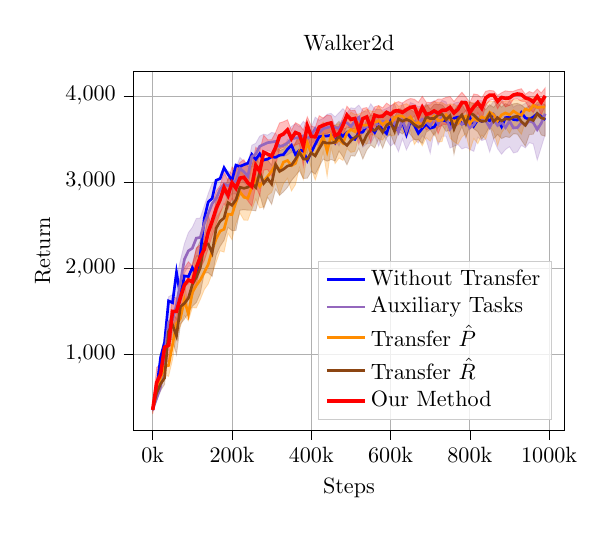
\begin{tikzpicture}[scale=0.8]

\definecolor{color0}{rgb}{1,0.549019607843137,0}
% \definecolor{color1}{rgb}{0.501960784313725,0,0.501960784313725}
% \definecolor{color1}{rgb}{0.4,0.69803921568,1}
\definecolor{color1}{rgb}{0.55,0.27,0.07}
\definecolor{color2}{rgb}{0.580392156862745,0.403921568627451,0.741176470588235}
\begin{axis}[
legend cell align={left},
legend style={
  fill opacity=0.8,
  draw opacity=1,
  text opacity=1,
  at={(0.97,0.03)},
  anchor=south east,
  draw=white!80!black
},
tick align=outside,
tick pos=left,
title={{Walker2d}},
x grid style={white!69.0196078431373!black},
xlabel={{Steps}},
xmajorgrids,
xmin=-4.95, xmax=103.95,
xtick style={color=black},
xtick={0,20,40,60,80,100},
xticklabels={0k,200k,400k,600k,800k,1000k},
y grid style={white!69.0196078431373!black},
ymajorgrids,
ylabel={{Return}},
ymin=115.808622308108, ymax=4283.96550845008,
ytick style={color=black}
]


\path [draw=color2, fill=color2, opacity=0.25]
(axis cs:0,370.375706469879)
--(axis cs:0,342.173368712645)
--(axis cs:1,462.493904964554)
--(axis cs:2,567.763321910152)
--(axis cs:3,808.302838079512)
--(axis cs:4,1089.86375496446)
--(axis cs:5,1117.82074532575)
--(axis cs:6,1283.65583272598)
--(axis cs:7,1625.98438667063)
--(axis cs:8,1942.45901285881)
--(axis cs:9,2019.8363617525)
--(axis cs:10,2027.81750798964)
--(axis cs:11,2134.04908171328)
--(axis cs:12,2138.66475923353)
--(axis cs:13,2314.39054285271)
--(axis cs:14,2430.38076721936)
--(axis cs:15,2504.66888628962)
--(axis cs:16,2603.29102780053)
--(axis cs:17,2798.72887494413)
--(axis cs:18,2867.93862451974)
--(axis cs:19,2798.9353273827)
--(axis cs:20,2861.09718099884)
--(axis cs:21,2862.73974988716)
--(axis cs:22,3028.71807335413)
--(axis cs:23,2996.73572051634)
--(axis cs:24,2945.49823769387)
--(axis cs:25,3174.69939669545)
--(axis cs:26,3188.72732409485)
--(axis cs:27,3299.60312049873)
--(axis cs:28,3318.25701153442)
--(axis cs:29,3367.22389293066)
--(axis cs:30,3348.85737689708)
--(axis cs:31,3374.98190578393)
--(axis cs:32,3338.39710447003)
--(axis cs:33,3294.86090693508)
--(axis cs:34,3315.76498877397)
--(axis cs:35,3344.01407516874)
--(axis cs:36,3341.42475146667)
--(axis cs:37,3379.31724188496)
--(axis cs:38,3359.24215805595)
--(axis cs:39,3334.8623696127)
--(axis cs:40,3447.3170068277)
--(axis cs:41,3482.09987230918)
--(axis cs:42,3396.48703908898)
--(axis cs:43,3501.60654154344)
--(axis cs:44,3454.37716229063)
--(axis cs:45,3484.45361525781)
--(axis cs:46,3493.87476061183)
--(axis cs:47,3418.14975220421)
--(axis cs:48,3525.84929567807)
--(axis cs:49,3555.80451660028)
--(axis cs:50,3446.28362360832)
--(axis cs:51,3548.66301666026)
--(axis cs:52,3598.07381830421)
--(axis cs:53,3404.63803328268)
--(axis cs:54,3447.30508683823)
--(axis cs:55,3449.65589451937)
--(axis cs:56,3535.40333887785)
--(axis cs:57,3416.11625829072)
--(axis cs:58,3553.46732849232)
--(axis cs:59,3491.87395009043)
--(axis cs:60,3417.59077759741)
--(axis cs:61,3455.69096862899)
--(axis cs:62,3353.07664466514)
--(axis cs:63,3503.94509946346)
--(axis cs:64,3373.12205891938)
--(axis cs:65,3469.29699995993)
--(axis cs:66,3499.37118905065)
--(axis cs:67,3454.38180354336)
--(axis cs:68,3538.55050766347)
--(axis cs:69,3489.66723235562)
--(axis cs:70,3333.14982143965)
--(axis cs:71,3595.38997444552)
--(axis cs:72,3431.65495823163)
--(axis cs:73,3532.10040880755)
--(axis cs:74,3532.13368287241)
--(axis cs:75,3395.21339879768)
--(axis cs:76,3416.2659327915)
--(axis cs:77,3435.28728914476)
--(axis cs:78,3384.10203226492)
--(axis cs:79,3403.25507463606)
--(axis cs:80,3379.96633837191)
--(axis cs:81,3356.44804517931)
--(axis cs:82,3521.56561111427)
--(axis cs:83,3481.55792838004)
--(axis cs:84,3498.37972027638)
--(axis cs:85,3348.16759229853)
--(axis cs:86,3496.51972803828)
--(axis cs:87,3386.65845178629)
--(axis cs:88,3322.81066580138)
--(axis cs:89,3377.71938248222)
--(axis cs:90,3410.24812308713)
--(axis cs:91,3337.8312744384)
--(axis cs:92,3350.01209086102)
--(axis cs:93,3427.09457979101)
--(axis cs:94,3397.42182301287)
--(axis cs:95,3457.35282874762)
--(axis cs:96,3443.014264011)
--(axis cs:97,3255.58761216463)
--(axis cs:98,3402.31203903516)
--(axis cs:99,3551.42348707499)
--(axis cs:99,3991.59285906436)
--(axis cs:99,3991.59285906436)
--(axis cs:98,3922.50371724036)
--(axis cs:97,3895.60758761068)
--(axis cs:96,3909.73541027615)
--(axis cs:95,3944.54092955533)
--(axis cs:94,3915.08488422152)
--(axis cs:93,3888.25848480454)
--(axis cs:92,3897.85239946243)
--(axis cs:91,3870.07349514349)
--(axis cs:90,3945.82036743784)
--(axis cs:89,3878.4694909515)
--(axis cs:88,3966.21306224804)
--(axis cs:87,3909.67670579407)
--(axis cs:86,3941.1545530123)
--(axis cs:85,3872.95116690488)
--(axis cs:84,3905.67717315887)
--(axis cs:83,3944.28954588994)
--(axis cs:82,3950.04471255965)
--(axis cs:81,3911.91612348903)
--(axis cs:80,3833.30290538064)
--(axis cs:79,3952.35886424045)
--(axis cs:78,3931.47283933706)
--(axis cs:77,3928.59434527728)
--(axis cs:76,3915.41034166115)
--(axis cs:75,3813.80906921131)
--(axis cs:74,3930.98191971403)
--(axis cs:73,3948.69156034768)
--(axis cs:72,3892.42890470976)
--(axis cs:71,3946.47090397837)
--(axis cs:70,3913.85187817861)
--(axis cs:69,3884.56962093558)
--(axis cs:68,3890.15115635557)
--(axis cs:67,3873.84322756943)
--(axis cs:66,3904.18044044327)
--(axis cs:65,3924.43133125279)
--(axis cs:64,3798.06479310637)
--(axis cs:63,3917.60538596156)
--(axis cs:62,3789.46628027542)
--(axis cs:61,3907.37623289664)
--(axis cs:60,3880.72606522257)
--(axis cs:59,3855.1715439021)
--(axis cs:58,3835.54074709961)
--(axis cs:57,3843.15587889968)
--(axis cs:56,3845.49372882243)
--(axis cs:55,3909.06736845202)
--(axis cs:54,3814.75199258378)
--(axis cs:53,3826.12918710761)
--(axis cs:52,3893.87963816858)
--(axis cs:51,3855.05221764679)
--(axis cs:50,3862.40025503683)
--(axis cs:49,3800.22754714129)
--(axis cs:48,3853.17342027581)
--(axis cs:47,3806.32550047094)
--(axis cs:46,3756.09252717373)
--(axis cs:45,3797.23026069552)
--(axis cs:44,3787.60267682417)
--(axis cs:43,3739.80661250088)
--(axis cs:42,3717.14325672657)
--(axis cs:41,3753.32444381442)
--(axis cs:40,3636.3443885278)
--(axis cs:39,3664.26225235737)
--(axis cs:38,3704.89345934524)
--(axis cs:37,3641.76183045561)
--(axis cs:36,3677.08626961294)
--(axis cs:35,3645.7023437611)
--(axis cs:34,3592.79732976273)
--(axis cs:33,3541.2638290813)
--(axis cs:32,3493.30838946763)
--(axis cs:31,3565.84411914016)
--(axis cs:30,3575.9053979094)
--(axis cs:29,3544.76888152162)
--(axis cs:28,3555.73325723988)
--(axis cs:27,3532.96465023261)
--(axis cs:26,3449.92365144134)
--(axis cs:25,3426.28346225615)
--(axis cs:24,3204.03974607287)
--(axis cs:23,3240.58962974916)
--(axis cs:22,3285.96166679443)
--(axis cs:21,3161.83033990988)
--(axis cs:20,3099.86124710482)
--(axis cs:19,3129.71106321335)
--(axis cs:18,3081.4652805466)
--(axis cs:17,3026.2286253186)
--(axis cs:16,3020.48931986398)
--(axis cs:15,2988.45325380023)
--(axis cs:14,2863.3212833067)
--(axis cs:13,2720.63878542292)
--(axis cs:12,2581.81087185593)
--(axis cs:11,2575.57970436256)
--(axis cs:10,2474.02440326987)
--(axis cs:9,2411.17098800992)
--(axis cs:8,2282.2798553823)
--(axis cs:7,2093.74688361311)
--(axis cs:6,1888.17273740721)
--(axis cs:5,1690.71040749618)
--(axis cs:4,1666.15628659667)
--(axis cs:3,1206.27742982685)
--(axis cs:2,678.452142974261)
--(axis cs:1,513.306303849133)
--(axis cs:0,370.375706469879)
--cycle;

\path [draw=color0, fill=color0, opacity=0.25]
(axis cs:0,367.856351844657)
--(axis cs:0,331.7895250355)
--(axis cs:1,542.749390564342)
--(axis cs:2,606.082189314856)
--(axis cs:3,765.680882108329)
--(axis cs:4,739.473775594633)
--(axis cs:5,934.945118186632)
--(axis cs:6,1227.77732343697)
--(axis cs:7,1323.49246722229)
--(axis cs:8,1449.48972938041)
--(axis cs:9,1388.02286792268)
--(axis cs:10,1539.59390793494)
--(axis cs:11,1535.90829342556)
--(axis cs:12,1633.89670415609)
--(axis cs:13,1748.12431558777)
--(axis cs:14,1815.14391503377)
--(axis cs:15,1936.74617636667)
--(axis cs:16,2065.98852865256)
--(axis cs:17,2200.8488039621)
--(axis cs:18,2185.23452101243)
--(axis cs:19,2403.35326641465)
--(axis cs:20,2329.98686137017)
--(axis cs:21,2519.7401999646)
--(axis cs:22,2637.04596981122)
--(axis cs:23,2557.53546128018)
--(axis cs:24,2555.00047032547)
--(axis cs:25,2680.36823678592)
--(axis cs:26,2802.87111423073)
--(axis cs:27,2697.96673955377)
--(axis cs:28,2711.39290152001)
--(axis cs:29,2844.09155735304)
--(axis cs:30,2879.76164004849)
--(axis cs:31,3011.55513939494)
--(axis cs:32,2854.71904693517)
--(axis cs:33,2983.26766226702)
--(axis cs:34,3043.13635692258)
--(axis cs:35,2895.72456778264)
--(axis cs:36,2968.80519850959)
--(axis cs:37,3171.00324900028)
--(axis cs:38,3030.19983269196)
--(axis cs:39,3342.795455005)
--(axis cs:40,3155.91372183805)
--(axis cs:41,3023.5085856405)
--(axis cs:42,3163.66759203856)
--(axis cs:43,3354.67982706243)
--(axis cs:44,3064.69467140258)
--(axis cs:45,3403.99876581115)
--(axis cs:46,3214.02286334236)
--(axis cs:47,3278.3091359412)
--(axis cs:48,3250.515802417)
--(axis cs:49,3390.54001034724)
--(axis cs:50,3344.26403859633)
--(axis cs:51,3357.37141472994)
--(axis cs:52,3523.17760028126)
--(axis cs:53,3473.12817140661)
--(axis cs:54,3440.7024694207)
--(axis cs:55,3551.87945136366)
--(axis cs:56,3541.47472851054)
--(axis cs:57,3503.33545989816)
--(axis cs:58,3487.25132674486)
--(axis cs:59,3562.63180271737)
--(axis cs:60,3537.37776956138)
--(axis cs:61,3538.04958107584)
--(axis cs:62,3630.5308767835)
--(axis cs:63,3589.12340291787)
--(axis cs:64,3515.11321481038)
--(axis cs:65,3603.90255458416)
--(axis cs:66,3435.58973744496)
--(axis cs:67,3500.30258546558)
--(axis cs:68,3421.77050898191)
--(axis cs:69,3514.75924974354)
--(axis cs:70,3474.04551708519)
--(axis cs:71,3571.14641045148)
--(axis cs:72,3463.20902583544)
--(axis cs:73,3470.32501927436)
--(axis cs:74,3655.22532247621)
--(axis cs:75,3512.11509734924)
--(axis cs:76,3467.87770227842)
--(axis cs:77,3439.27834784486)
--(axis cs:78,3523.84120227783)
--(axis cs:79,3562.26239513997)
--(axis cs:80,3363.86576569324)
--(axis cs:81,3506.01897477167)
--(axis cs:82,3444.74052443256)
--(axis cs:83,3545.45030117038)
--(axis cs:84,3498.25301003705)
--(axis cs:85,3649.54119325088)
--(axis cs:86,3585.87602503182)
--(axis cs:87,3422.34677737147)
--(axis cs:88,3570.2922288671)
--(axis cs:89,3639.79705122712)
--(axis cs:90,3564.93990205729)
--(axis cs:91,3659.53093738392)
--(axis cs:92,3615.20662868987)
--(axis cs:93,3553.34504085755)
--(axis cs:94,3698.35614124499)
--(axis cs:95,3695.63608905316)
--(axis cs:96,3786.93825029959)
--(axis cs:97,3738.41640245298)
--(axis cs:98,3762.04833625575)
--(axis cs:99,3777.65881120799)
--(axis cs:99,3963.85100467454)
--(axis cs:99,3963.85100467454)
--(axis cs:98,3969.49938231468)
--(axis cs:97,3995.29783060159)
--(axis cs:96,3986.71579775184)
--(axis cs:95,3954.51884428005)
--(axis cs:94,3978.44240989225)
--(axis cs:93,3950.78197875521)
--(axis cs:92,3953.44460757998)
--(axis cs:91,3956.87060810095)
--(axis cs:90,3943.44058813081)
--(axis cs:89,3941.24567665442)
--(axis cs:88,3933.16085505911)
--(axis cs:87,3939.9619813746)
--(axis cs:86,3934.19839974407)
--(axis cs:85,3940.78829566094)
--(axis cs:84,3910.77634343594)
--(axis cs:83,3921.74837563452)
--(axis cs:82,3904.33084269199)
--(axis cs:81,3919.0403852433)
--(axis cs:80,3926.59586086718)
--(axis cs:79,3930.76186765801)
--(axis cs:78,3902.17527545988)
--(axis cs:77,3873.72759856422)
--(axis cs:76,3905.15382480952)
--(axis cs:75,3907.84402842145)
--(axis cs:74,3894.15898783792)
--(axis cs:73,3921.77371099833)
--(axis cs:72,3923.34722170849)
--(axis cs:71,3936.5462491727)
--(axis cs:70,3893.33003190487)
--(axis cs:69,3886.87435268664)
--(axis cs:68,3838.03936576636)
--(axis cs:67,3852.32258770516)
--(axis cs:66,3880.41354024706)
--(axis cs:65,3882.2067014306)
--(axis cs:64,3910.30194514937)
--(axis cs:63,3894.98404138551)
--(axis cs:62,3879.12993274511)
--(axis cs:61,3930.74254850122)
--(axis cs:60,3773.65869645193)
--(axis cs:59,3828.24780697308)
--(axis cs:58,3812.37080497638)
--(axis cs:57,3885.50064803991)
--(axis cs:56,3817.39191808463)
--(axis cs:55,3827.03098123976)
--(axis cs:54,3845.18184686881)
--(axis cs:53,3810.49901209327)
--(axis cs:52,3790.60443878978)
--(axis cs:51,3784.93587323426)
--(axis cs:50,3812.90933999158)
--(axis cs:49,3728.7414007127)
--(axis cs:48,3621.76931351139)
--(axis cs:47,3677.73450739621)
--(axis cs:46,3657.4741726251)
--(axis cs:45,3664.94767042935)
--(axis cs:44,3624.49811674399)
--(axis cs:43,3697.18818852939)
--(axis cs:42,3644.75476683708)
--(axis cs:41,3571.53128075957)
--(axis cs:40,3524.82569456544)
--(axis cs:39,3582.22758823641)
--(axis cs:38,3522.24580457439)
--(axis cs:37,3528.41726464333)
--(axis cs:36,3447.26266300422)
--(axis cs:35,3427.54849374586)
--(axis cs:34,3456.28573039965)
--(axis cs:33,3450.0097682493)
--(axis cs:32,3382.05380952829)
--(axis cs:31,3385.24677153073)
--(axis cs:30,3347.84476086246)
--(axis cs:29,3295.20780419495)
--(axis cs:28,3256.90515666412)
--(axis cs:27,3217.59138375875)
--(axis cs:26,3280.08719671192)
--(axis cs:25,3196.74488426592)
--(axis cs:24,3083.72757727848)
--(axis cs:23,3078.79634199645)
--(axis cs:22,3153.59984501238)
--(axis cs:21,3020.35243049585)
--(axis cs:20,2867.35321876242)
--(axis cs:19,2852.06841912104)
--(axis cs:18,2712.89192949541)
--(axis cs:17,2654.19625754519)
--(axis cs:16,2581.6463746823)
--(axis cs:15,2471.76074787688)
--(axis cs:14,2282.70745813486)
--(axis cs:13,2170.4961120927)
--(axis cs:12,2148.97358886023)
--(axis cs:11,2146.08730636037)
--(axis cs:10,1931.23947121497)
--(axis cs:9,1535.37271125176)
--(axis cs:8,1837.95586289953)
--(axis cs:7,1503.64983788043)
--(axis cs:6,1482.94122336036)
--(axis cs:5,1274.79752362669)
--(axis cs:4,991.034662723162)
--(axis cs:3,947.81732026937)
--(axis cs:2,861.803551641503)
--(axis cs:1,600.238556602336)
--(axis cs:0,367.856351844657)
--cycle;

\path [draw=color1, fill=color1, opacity=0.25]
(axis cs:0,384.487725901216)
--(axis cs:0,349.262693091479)
--(axis cs:1,491.638093860051)
--(axis cs:2,576.229846551738)
--(axis cs:3,648.955526798417)
--(axis cs:4,1171.86833251252)
--(axis cs:5,1164.56572405792)
--(axis cs:6,994.617881080697)
--(axis cs:7,1350.49271719613)
--(axis cs:8,1406.10209462812)
--(axis cs:9,1483.92128276943)
--(axis cs:10,1555.65791158369)
--(axis cs:11,1599.25063312176)
--(axis cs:12,1704.95719758964)
--(axis cs:13,1939.46044852897)
--(axis cs:14,1946.08751545455)
--(axis cs:15,1902.53132395036)
--(axis cs:16,2148.73786896812)
--(axis cs:17,2252.23667163637)
--(axis cs:18,2322.66643230518)
--(axis cs:19,2474.02725904349)
--(axis cs:20,2435.05281508411)
--(axis cs:21,2437.1410729301)
--(axis cs:22,2672.34660626664)
--(axis cs:23,2677.80475655762)
--(axis cs:24,2672.58462189355)
--(axis cs:25,2671.79357742089)
--(axis cs:26,2664.85951336713)
--(axis cs:27,2856.05226360745)
--(axis cs:28,2690.04852601567)
--(axis cs:29,2822.16609543725)
--(axis cs:30,2740.39984007289)
--(axis cs:31,2916.85434699396)
--(axis cs:32,2844.81999816954)
--(axis cs:33,2888.0232668731)
--(axis cs:34,2938.56327218846)
--(axis cs:35,3016.75490195306)
--(axis cs:36,3071.89136641257)
--(axis cs:37,3131.60464832291)
--(axis cs:38,3041.20744644538)
--(axis cs:39,3044.83580590062)
--(axis cs:40,3124.14121273659)
--(axis cs:41,3090.63278578131)
--(axis cs:42,3179.99655985625)
--(axis cs:43,3266.72034171356)
--(axis cs:44,3242.19002760564)
--(axis cs:45,3261.41261380786)
--(axis cs:46,3243.67917066495)
--(axis cs:47,3359.8412796876)
--(axis cs:48,3292.91878318438)
--(axis cs:49,3201.12241666796)
--(axis cs:50,3306.50967967612)
--(axis cs:51,3300.52637606659)
--(axis cs:52,3392.08508084944)
--(axis cs:53,3266.94217887651)
--(axis cs:54,3372.85076584166)
--(axis cs:55,3431.4435510105)
--(axis cs:56,3396.09164820547)
--(axis cs:57,3506.38685128661)
--(axis cs:58,3394.51655900642)
--(axis cs:59,3517.76343486616)
--(axis cs:60,3557.14478614956)
--(axis cs:61,3438.19272761633)
--(axis cs:62,3587.9830999042)
--(axis cs:63,3557.68142199972)
--(axis cs:64,3611.52972376149)
--(axis cs:65,3550.73120964701)
--(axis cs:66,3494.54416039157)
--(axis cs:67,3490.84845319256)
--(axis cs:68,3448.0675194065)
--(axis cs:69,3578.35972400253)
--(axis cs:70,3610.01950744789)
--(axis cs:71,3538.29966196876)
--(axis cs:72,3634.75474045207)
--(axis cs:73,3659.41738579462)
--(axis cs:74,3588.10552976163)
--(axis cs:75,3605.56651176904)
--(axis cs:76,3322.7528837024)
--(axis cs:77,3538.19909065727)
--(axis cs:78,3644.72359020858)
--(axis cs:79,3513.56561580097)
--(axis cs:80,3655.09463365858)
--(axis cs:81,3619.02097746319)
--(axis cs:82,3584.88364220171)
--(axis cs:83,3496.24211321349)
--(axis cs:84,3562.93657373327)
--(axis cs:85,3654.58936834051)
--(axis cs:86,3502.53788154698)
--(axis cs:87,3552.94405713209)
--(axis cs:88,3504.71246100757)
--(axis cs:89,3527.33383563834)
--(axis cs:90,3517.64276496953)
--(axis cs:91,3560.80396112477)
--(axis cs:92,3556.10784819381)
--(axis cs:93,3486.65972531057)
--(axis cs:94,3417.46766854692)
--(axis cs:95,3551.87480738684)
--(axis cs:96,3555.70020222342)
--(axis cs:97,3651.76450390132)
--(axis cs:98,3546.69568834868)
--(axis cs:99,3532.57990316061)
--(axis cs:99,3896.42993899305)
--(axis cs:99,3896.42993899305)
--(axis cs:98,3915.69433442594)
--(axis cs:97,3926.70536737998)
--(axis cs:96,3866.52343325955)
--(axis cs:95,3887.48248953416)
--(axis cs:94,3854.54769616803)
--(axis cs:93,3895.4905798975)
--(axis cs:92,3914.72063632228)
--(axis cs:91,3908.55453530984)
--(axis cs:90,3889.45047412929)
--(axis cs:89,3911.74180848471)
--(axis cs:88,3870.26736111725)
--(axis cs:87,3919.72675550692)
--(axis cs:86,3867.14369832714)
--(axis cs:85,3899.86223507278)
--(axis cs:84,3841.07964615196)
--(axis cs:83,3882.56673196854)
--(axis cs:82,3863.42941241875)
--(axis cs:81,3911.21235947546)
--(axis cs:80,3924.92632813463)
--(axis cs:79,3824.64302902067)
--(axis cs:78,3902.31597054257)
--(axis cs:77,3895.44322796199)
--(axis cs:76,3830.86717107863)
--(axis cs:75,3899.94333830604)
--(axis cs:74,3848.38180419919)
--(axis cs:73,3896.03244512739)
--(axis cs:72,3903.95371773781)
--(axis cs:71,3900.27126165423)
--(axis cs:70,3845.52327367146)
--(axis cs:69,3913.69547687514)
--(axis cs:68,3814.21251608101)
--(axis cs:67,3781.67391359021)
--(axis cs:66,3811.58292325813)
--(axis cs:65,3843.76873987044)
--(axis cs:64,3824.82938047989)
--(axis cs:63,3837.13350786105)
--(axis cs:62,3855.63484544816)
--(axis cs:61,3749.91032879795)
--(axis cs:60,3800.34472114423)
--(axis cs:59,3791.63406352863)
--(axis cs:58,3744.70033051974)
--(axis cs:57,3762.34244083795)
--(axis cs:56,3771.78095293694)
--(axis cs:55,3777.13385506671)
--(axis cs:54,3726.27233571461)
--(axis cs:53,3614.38587422835)
--(axis cs:52,3699.75515543258)
--(axis cs:51,3705.00311157444)
--(axis cs:50,3651.51267330569)
--(axis cs:49,3630.56222655236)
--(axis cs:48,3616.81280112556)
--(axis cs:47,3706.01842907628)
--(axis cs:46,3658.49700533447)
--(axis cs:45,3645.5586413327)
--(axis cs:44,3623.33754975534)
--(axis cs:43,3641.57833359002)
--(axis cs:42,3591.46828534213)
--(axis cs:41,3521.78433907192)
--(axis cs:40,3574.78516798828)
--(axis cs:39,3481.32515015187)
--(axis cs:38,3486.14491661857)
--(axis cs:37,3561.78611203791)
--(axis cs:36,3458.42189320984)
--(axis cs:35,3359.01841089155)
--(axis cs:34,3436.92888545621)
--(axis cs:33,3384.96217967241)
--(axis cs:32,3363.56141339884)
--(axis cs:31,3459.07338864447)
--(axis cs:30,3196.82792674707)
--(axis cs:29,3253.47932709641)
--(axis cs:28,3251.74237669036)
--(axis cs:27,3347.44206477354)
--(axis cs:26,3218.17182710655)
--(axis cs:25,3287.77244645031)
--(axis cs:24,3199.28379440167)
--(axis cs:23,3193.0450379031)
--(axis cs:22,3204.42777774483)
--(axis cs:21,3124.37702856815)
--(axis cs:20,3017.12073815743)
--(axis cs:19,3046.49258482822)
--(axis cs:18,2872.93672987232)
--(axis cs:17,2831.69372290441)
--(axis cs:16,2804.05161179734)
--(axis cs:15,2461.77563511273)
--(axis cs:14,2609.8660111885)
--(axis cs:13,2604.25234193571)
--(axis cs:12,2316.63806422931)
--(axis cs:11,2220.56776885352)
--(axis cs:10,2050.75243191151)
--(axis cs:9,1816.48664903717)
--(axis cs:8,1791.46312867217)
--(axis cs:7,1742.98218414771)
--(axis cs:6,1406.71594975329)
--(axis cs:5,1489.60527681403)
--(axis cs:4,1365.71795123707)
--(axis cs:3,804.091125274206)
--(axis cs:2,762.151728266336)
--(axis cs:1,611.862393743629)
--(axis cs:0,384.487725901216)
--cycle;
\path [draw=red, fill=red, opacity=0.25]
(axis cs:0,407.533710470678)
--(axis cs:0,305.270298950925)
--(axis cs:1,537.532566200477)
--(axis cs:2,658.555372768738)
--(axis cs:3,944.768609914622)
--(axis cs:4,907.039772626741)
--(axis cs:5,1320.42208426518)
--(axis cs:6,1341.39208711135)
--(axis cs:7,1548.19228135746)
--(axis cs:8,1633.85555078248)
--(axis cs:9,1669.58278034828)
--(axis cs:10,1674.51217992106)
--(axis cs:11,1811.5678847737)
--(axis cs:12,1995.7528165432)
--(axis cs:13,2085.76752501497)
--(axis cs:14,2226.10315310418)
--(axis cs:15,2374.23989895114)
--(axis cs:16,2512.471867885)
--(axis cs:17,2634.42884041164)
--(axis cs:18,2750.94117121601)
--(axis cs:19,2686.36199158847)
--(axis cs:20,2810.09333474585)
--(axis cs:21,2740.49990260902)
--(axis cs:22,2853.47612562619)
--(axis cs:23,2845.02069031175)
--(axis cs:24,2782.01319168169)
--(axis cs:25,2718.88819529182)
--(axis cs:26,2956.51948302525)
--(axis cs:27,2840.40062604605)
--(axis cs:28,3137.95570042929)
--(axis cs:29,3145.88378721824)
--(axis cs:30,3065.50469678833)
--(axis cs:31,3190.69743896604)
--(axis cs:32,3385.08844823865)
--(axis cs:33,3401.53806408227)
--(axis cs:34,3489.19308003916)
--(axis cs:35,3395.07805026134)
--(axis cs:36,3430.44634490144)
--(axis cs:37,3446.638448274)
--(axis cs:38,3184.76465553071)
--(axis cs:39,3530.86059606125)
--(axis cs:40,3399.18400724134)
--(axis cs:41,3407.83478588424)
--(axis cs:42,3507.86713130122)
--(axis cs:43,3562.65084771154)
--(axis cs:44,3564.16108699171)
--(axis cs:45,3583.90921552952)
--(axis cs:46,3431.86540281412)
--(axis cs:47,3476.08872074995)
--(axis cs:48,3548.9733909679)
--(axis cs:49,3650.64280084877)
--(axis cs:50,3617.37194100812)
--(axis cs:51,3624.17268740678)
--(axis cs:52,3437.56898875566)
--(axis cs:53,3599.77523538695)
--(axis cs:54,3608.57216806922)
--(axis cs:55,3458.79617507407)
--(axis cs:56,3661.55564905219)
--(axis cs:57,3602.42811245603)
--(axis cs:58,3646.84518397833)
--(axis cs:59,3686.97885036873)
--(axis cs:60,3678.81387508645)
--(axis cs:61,3690.79691338848)
--(axis cs:62,3712.95556641836)
--(axis cs:63,3674.24342413673)
--(axis cs:64,3704.45447734433)
--(axis cs:65,3725.121310352)
--(axis cs:66,3767.71026515808)
--(axis cs:67,3560.77843711689)
--(axis cs:68,3715.07166425761)
--(axis cs:69,3603.12180897819)
--(axis cs:70,3630.68793467386)
--(axis cs:71,3700.61845954175)
--(axis cs:72,3560.12732371397)
--(axis cs:73,3671.94297242452)
--(axis cs:74,3666.52192767139)
--(axis cs:75,3722.9750825507)
--(axis cs:76,3635.27585189935)
--(axis cs:77,3664.04966900103)
--(axis cs:78,3772.23867325207)
--(axis cs:79,3832.76872698679)
--(axis cs:80,3666.05076812306)
--(axis cs:81,3655.61450543928)
--(axis cs:82,3805.57201923473)
--(axis cs:83,3715.78889329693)
--(axis cs:84,3891.44094003287)
--(axis cs:85,3948.91039684973)
--(axis cs:86,3959.63072474719)
--(axis cs:87,3851.195867319)
--(axis cs:88,3928.0970572451)
--(axis cs:89,3872.71557233753)
--(axis cs:90,3891.65612060109)
--(axis cs:91,3963.42992780049)
--(axis cs:92,3966.01519154662)
--(axis cs:93,3938.44623564186)
--(axis cs:94,3936.17382700384)
--(axis cs:95,3858.52355732583)
--(axis cs:96,3806.41364701511)
--(axis cs:97,3890.93449130692)
--(axis cs:98,3779.81574641154)
--(axis cs:99,3884.28074710913)
--(axis cs:99,4094.50383180726)
--(axis cs:99,4094.50383180726)
--(axis cs:98,4034.23441882702)
--(axis cs:97,4080.10576272014)
--(axis cs:96,4033.6490998368)
--(axis cs:95,4051.74749901585)
--(axis cs:94,4018.70808147539)
--(axis cs:93,4084.2440877742)
--(axis cs:92,4072.02577084672)
--(axis cs:91,4055.53540248013)
--(axis cs:90,4052.17713909033)
--(axis cs:89,4059.47260816945)
--(axis cs:88,4037.10789242985)
--(axis cs:87,4007.2874138841)
--(axis cs:86,4059.06528867849)
--(axis cs:85,4064.50979860463)
--(axis cs:84,4055.00056665817)
--(axis cs:83,3976.80555866988)
--(axis cs:82,4014.21971006857)
--(axis cs:81,4023.56722761994)
--(axis cs:80,3924.73335454392)
--(axis cs:79,3987.57400450726)
--(axis cs:78,4043.27653026183)
--(axis cs:77,3991.14150541446)
--(axis cs:76,3936.026370433)
--(axis cs:75,3992.55172075333)
--(axis cs:74,3984.01939752545)
--(axis cs:73,3964.18344886101)
--(axis cs:72,3965.02728077486)
--(axis cs:71,3935.01659309285)
--(axis cs:70,3923.43932677333)
--(axis cs:69,3927.46331746483)
--(axis cs:68,3995.61999551437)
--(axis cs:67,3926.25475228484)
--(axis cs:66,3962.33842326475)
--(axis cs:65,3970.33315759355)
--(axis cs:64,3951.25012123968)
--(axis cs:63,3916.76978494134)
--(axis cs:62,3934.72130734052)
--(axis cs:61,3917.14255610038)
--(axis cs:60,3884.6141572353)
--(axis cs:59,3916.35203797914)
--(axis cs:58,3861.09134854442)
--(axis cs:57,3888.76602216235)
--(axis cs:56,3873.61383559934)
--(axis cs:55,3777.27400595311)
--(axis cs:54,3865.60197677936)
--(axis cs:53,3855.46824216789)
--(axis cs:52,3729.49204148612)
--(axis cs:51,3836.82973624683)
--(axis cs:50,3828.53598087851)
--(axis cs:49,3881.21708166457)
--(axis cs:48,3753.23500591823)
--(axis cs:47,3647.44160941715)
--(axis cs:46,3640.62105980395)
--(axis cs:45,3770.1011719949)
--(axis cs:44,3777.83094066801)
--(axis cs:43,3743.72805239768)
--(axis cs:42,3770.2853342693)
--(axis cs:41,3633.54293874471)
--(axis cs:40,3651.15681826498)
--(axis cs:39,3757.50337269418)
--(axis cs:38,3604.00350663062)
--(axis cs:37,3664.59441056387)
--(axis cs:36,3689.77732626202)
--(axis cs:35,3598.36548381147)
--(axis cs:34,3722.63275268238)
--(axis cs:33,3701.46183431704)
--(axis cs:32,3686.47592271597)
--(axis cs:31,3575.38955450296)
--(axis cs:30,3491.75907400038)
--(axis cs:29,3490.26698904868)
--(axis cs:28,3543.68939853356)
--(axis cs:27,3364.04984194389)
--(axis cs:26,3403.22704694552)
--(axis cs:25,3186.49185473395)
--(axis cs:24,3178.98179844641)
--(axis cs:23,3260.31181559133)
--(axis cs:22,3226.63667444338)
--(axis cs:21,3141.72143145636)
--(axis cs:20,3174.82198521341)
--(axis cs:19,3017.71506730689)
--(axis cs:18,3116.05256954178)
--(axis cs:17,2957.6050845039)
--(axis cs:16,2894.23597262589)
--(axis cs:15,2732.55279992138)
--(axis cs:14,2602.02701567098)
--(axis cs:13,2356.9238586003)
--(axis cs:12,2267.02353213471)
--(axis cs:11,2235.23547596398)
--(axis cs:10,2022.13444485554)
--(axis cs:9,2073.72645041419)
--(axis cs:8,2001.80241216607)
--(axis cs:7,1777.18929485367)
--(axis cs:6,1646.78859718402)
--(axis cs:5,1674.02688751081)
--(axis cs:4,1293.19381542621)
--(axis cs:3,1208.99026802613)
--(axis cs:2,890.285880116113)
--(axis cs:1,844.927316475017)
--(axis cs:0,407.533710470678)
--cycle;
\addplot [very thick, blue]
table {%
0 348.786031833919
1 604.372654531799
2 965.047647917091
3 1141.69660008647
4 1618.28694840608
5 1596.55599625575
6 1952.32855563454
7 1669.33116436364
8 1908.51585553314
9 1900.95158684342
10 2003.17082548276
11 1920.20538511573
12 2158.11130943077
13 2574.24553846179
14 2768.0200348151
15 2809.54760060012
16 3019.81883820065
17 3040.16163239793
18 3165.75523530485
19 3089.41894932036
20 3020.07927677136
21 3196.32938510838
22 3179.34381523992
23 3201.23464495482
24 3218.10369254355
25 3320.89172537134
26 3262.21003847251
27 3328.78214367164
28 3255.55528762398
29 3266.20650105378
30 3292.7377156064
31 3286.60967093887
32 3310.47651794125
33 3319.26408629819
34 3381.10260887725
35 3427.21149494887
36 3318.83817062111
37 3367.99512185791
38 3364.03648793041
39 3249.15601363706
40 3345.69619432986
41 3438.65858767672
42 3526.53010425513
43 3533.54264765776
44 3535.20129057824
45 3543.55326213085
46 3460.49023333834
47 3569.82529089082
48 3531.85831803365
49 3576.53005790122
50 3512.77564113537
51 3495.10973956346
52 3575.85157529766
53 3579.1370592863
54 3657.94099634905
55 3639.41467911535
56 3575.70489982169
57 3665.80634234821
58 3605.73420160541
59 3562.71200214178
60 3707.05136255598
61 3630.09473767936
62 3597.70462679886
63 3697.21932683403
64 3553.88300570137
65 3702.16975230477
66 3658.5567645764
67 3565.43047857311
68 3622.30341915348
69 3673.54937018337
70 3625.02436670114
71 3638.86181351615
72 3713.39672556402
73 3719.81732209679
74 3710.57799145728
75 3671.88417165961
76 3741.85713274778
77 3754.28131394611
78 3674.68365474079
79 3689.63897085822
80 3749.7544466619
81 3651.1416426323
82 3721.57675631618
83 3704.91964361769
84 3738.35121783512
85 3711.33547133662
86 3781.49638300054
87 3721.35914679416
88 3642.34820588273
89 3748.02911624766
90 3753.77099811448
91 3725.36575573506
92 3720.12000647399
93 3806.74276355086
94 3745.54964887382
95 3727.84257022077
96 3755.68694817698
97 3793.25150246693
98 3760.91346089704
99 3721.92041298397
};
\addlegendentry{Without Transfer}

\addplot [very thick, color2]
table {%
0 354.998441434043
1 487.456722884113
2 626.102133430314
3 993.40045753288
4 1372.01951563316
5 1397.96000282088
6 1573.90160238139
7 1841.35700921823
8 2101.61315310599
9 2199.64924128657
10 2230.90797073997
11 2347.50641898431
12 2356.69280241553
13 2515.90860857775
14 2632.22424211953
15 2750.11966207629
16 2808.69113144779
17 2912.35361524246
18 2975.22211578254
19 2958.61284206689
20 2984.48480085725
21 3014.7413309254
22 3156.74319873248
23 3118.8636417434
24 3067.0334988589
25 3293.17207604071
26 3325.75704442137
27 3415.50112202548
28 3436.7377036597
29 3457.52185029762
30 3464.19217049385
31 3471.3964652664
32 3413.95641898105
33 3425.53935273139
34 3453.41536424215
35 3503.23789344732
36 3510.78302561517
37 3518.73891244199
38 3536.84612097209
39 3503.90422836195
40 3543.97775625686
41 3622.39805250382
42 3572.46891410924
43 3619.59573939181
44 3632.6220656587
45 3645.23807580612
46 3633.42062310596
47 3621.97394927098
48 3700.12703452548
49 3687.30363219434
50 3647.31219972896
51 3705.45555939774
52 3751.56789829024
53 3627.25575398223
54 3643.52206469824
55 3691.94424999499
56 3695.35874685519
57 3654.34838234083
58 3706.41411410129
59 3693.86103658809
60 3663.44286078916
61 3689.74513902695
62 3581.16593034799
63 3721.9190603133
64 3592.31798124848
65 3721.571876799
66 3702.98200443755
67 3684.58063347984
68 3730.82867440441
69 3701.84878212795
70 3654.4903965613
71 3779.52732889492
72 3673.90381752416
73 3758.43801988689
74 3751.78369856736
75 3616.23950755084
76 3676.986796104
77 3698.92386465317
78 3672.25748550819
79 3701.41440974953
80 3629.38762092454
81 3668.21939794884
82 3747.53253766881
83 3729.57885940172
84 3715.40260293304
85 3635.72823056108
86 3727.29902767929
87 3657.42127550056
88 3694.6121173739
89 3633.17755893516
90 3707.90009758295
91 3628.02589859599
92 3633.43765419393
93 3692.22895936264
94 3660.14248110664
95 3711.7033039817
96 3690.53925376232
97 3609.82385276299
98 3682.62394914161
99 3793.36941841728
};
\addlegendentry{Auxiliary Tasks}
\addplot [very thick, color0]
table {%
0 351.225076348745
1 569.656464521901
2 723.807667574152
3 858.418918809424
4 868.146844445558
5 1108.46271280393
6 1354.32613649095
7 1414.99339421318
8 1631.26076620632
9 1461.65246458663
10 1718.11190264894
11 1797.81226539717
12 1861.82266601557
13 1948.62632312377
14 2041.0429959157
15 2207.78753574577
16 2339.34717279421
17 2428.99058638904
18 2450.98588571585
19 2626.50840773999
20 2620.66712422881
21 2767.21527372937
22 2885.97128966208
23 2823.13823858791
24 2811.56383805857
25 2942.28399977312
26 3033.87614227804
27 2949.19379371141
28 3011.06121918644
29 3066.12376654483
30 3126.62263111907
31 3202.0602128438
32 3129.76496149842
33 3231.62652658393
34 3250.16876642129
35 3190.40730935011
36 3215.87033473234
37 3355.52813362476
38 3277.40381237662
39 3459.8001292671
40 3331.20765588148
41 3310.77783843531
42 3407.22291422917
43 3530.13043277758
44 3356.66775873996
45 3538.40026470877
46 3458.3283122696
47 3491.52480617566
48 3450.98997704571
49 3571.3900483483
50 3609.28982931993
51 3585.58069431566
52 3672.73270004548
53 3659.36154749126
54 3660.91167837684
55 3698.81469459137
56 3693.32792848466
57 3711.25176374404
58 3668.77814632654
59 3705.600107538
60 3672.53276536687
61 3749.22721578422
62 3768.9360337868
63 3765.77452411345
64 3721.11158655557
65 3756.8533854911
66 3681.76401414869
67 3692.8276300495
68 3652.79166070664
69 3713.96834977098
70 3705.86442916297
71 3769.8621300368
72 3714.19452851153
73 3717.76474013161
74 3779.84465156032
75 3724.14817211287
76 3709.48112161208
77 3683.47183613859
78 3736.24050711246
79 3765.53709253194
80 3679.53784699045
81 3740.68029773413
82 3711.83252760063
83 3756.79256476068
84 3737.1161079167
85 3810.99898608199
86 3783.56405471031
87 3710.87223881512
88 3780.73321772546
89 3802.5259068328
90 3781.48142106798
91 3823.8959378579
92 3793.6868132087
93 3775.61869840006
94 3847.71051695892
95 3831.28068762949
96 3893.12833371685
97 3866.18695501882
98 3870.52176602996
99 3871.04813466859
};
\addlegendentry{Transfer $\hat{P}$}
\addplot [very thick, color1]
table {%
0 365.336373355671
1 547.341350139598
2 654.810319077989
3 723.508785747305
4 1264.63985415444
5 1339.7964072474
6 1210.96412402802
7 1551.7751815685
8 1589.81480832584
9 1650.24811363773
10 1807.51492981558
11 1892.90670847867
12 2002.9004570512
13 2279.23506161303
14 2280.1483223308
15 2176.34767264894
16 2462.43672588921
17 2544.24572428884
18 2580.93933284141
19 2760.1010678933
20 2729.77558734906
21 2793.16480061559
22 2939.25611084345
23 2927.00956424984
24 2938.88049733465
25 2983.20623853321
26 2935.73695653633
27 3114.24700653549
28 2983.92686912795
29 3039.70833991062
30 2977.04438391621
31 3203.9541824593
32 3124.397826126
33 3148.60729496761
34 3185.87787717116
35 3196.13050592074
36 3263.80188099878
37 3344.07399404707
38 3268.21281051214
39 3267.23760052325
40 3339.05812343802
41 3303.88866418287
42 3387.93130734758
43 3464.55034202526
44 3451.60317126598
45 3453.44592515539
46 3461.88852385934
47 3537.14719158854
48 3464.26472986906
49 3425.90432926427
50 3483.35274061673
51 3517.70297902166
52 3550.18353475372
53 3448.27167058061
54 3546.23020618316
55 3611.25077273753
56 3599.88741082403
57 3643.24623056329
58 3577.31379740546
59 3659.1382705128
60 3691.63574407997
61 3591.01722152251
62 3734.24215077499
63 3706.57027144357
64 3728.33711605663
65 3707.0061454641
66 3666.54184985837
67 3636.53446184749
68 3654.61632131207
69 3760.43541012494
70 3736.8561224868
71 3738.22660832316
72 3778.87946489977
73 3788.93155537624
74 3722.13573694782
75 3770.66038840517
76 3617.38098216948
77 3731.64638163162
78 3780.06446501383
79 3676.99726085066
80 3802.02786190012
81 3779.54055416435
82 3731.49842708838
83 3704.96201333357
84 3709.00101931319
85 3790.99499377687
86 3700.99245277981
87 3746.7896932478
88 3710.21978590707
89 3734.9312935421
90 3729.15741670387
91 3756.20577035302
92 3764.05711436577
93 3702.0838784166
94 3659.50965707824
95 3734.93572146092
96 3714.9061973995
97 3795.58507556963
98 3744.64206985825
99 3733.0901786772
};
\addlegendentry{Transfer $\hat{R}$}
\addplot [ultra thick, red]
table {%
0 352.216536377132
1 668.803874193032
2 767.330976891019
3 1080.28835719827
4 1103.37156435703
5 1497.58734943897
6 1496.54393290749
7 1660.0384738353
8 1802.17997596836
9 1861.51654799798
10 1839.87962857442
11 2004.70091501243
12 2127.23195934199
13 2217.7279442298
14 2416.0409063133
15 2544.50231872939
16 2690.08645394612
17 2793.14551178875
18 2936.15087533605
19 2845.23227013396
20 2991.98059227674
21 2928.27851617842
22 3045.18086266371
23 3054.64980252015
24 2991.74772226943
25 2949.32102142374
26 3193.29223381274
27 3123.5535071955
28 3345.99625024637
29 3322.88181448398
30 3301.89817727821
31 3401.52459854713
32 3536.34733403601
33 3558.2441488628
34 3605.876582258
35 3504.53834872181
36 3575.19499243544
37 3555.5638813397
38 3418.40306346795
39 3652.78910578485
40 3530.37428050205
41 3524.825595245
42 3638.55984102108
43 3658.77951739737
44 3676.25503719853
45 3686.71610129983
46 3540.54339892823
47 3563.88035132998
48 3660.982560073
49 3776.48810509096
50 3727.28700125474
51 3738.69714686046
52 3594.50127071093
53 3736.55218993051
54 3756.09085847934
55 3628.42518013429
56 3775.90844720814
57 3761.57504069011
58 3766.54583356675
59 3809.24539968738
60 3785.68206787608
61 3824.81154549792
62 3827.09251812164
63 3808.78938620425
64 3841.56309126754
65 3867.35653142337
66 3875.51430263319
67 3762.95899324328
68 3868.11617117093
69 3784.91402568404
70 3797.93182028425
71 3826.59712351863
72 3798.60081531006
73 3833.63944346486
74 3836.15406515176
75 3866.35478835839
76 3803.19882782448
77 3844.36884046504
78 3925.57817062743
79 3919.5789011625
80 3807.52602500469
81 3872.99648786921
82 3923.64292448871
83 3857.23807969684
84 3976.51615745677
85 4009.74607755748
86 4010.7696615503
87 3938.22400235581
88 3982.79954975696
89 3972.18767697171
90 3977.78264037173
91 4011.36536878356
92 4023.36611127198
93 4015.93938203033
94 3977.60068088209
95 3963.15603348812
96 3931.55160639234
97 3995.59967511403
98 3927.14447251775
99 4000.74046488771
};
\addlegendentry{Our Method}
\end{axis}

\end{tikzpicture}
 
 \end{subfigure}
 \hfill
 \begin{subfigure}[t]{0.48\columnwidth}
  \centering
  % This file was created with tikzplotlib v0.9.12.
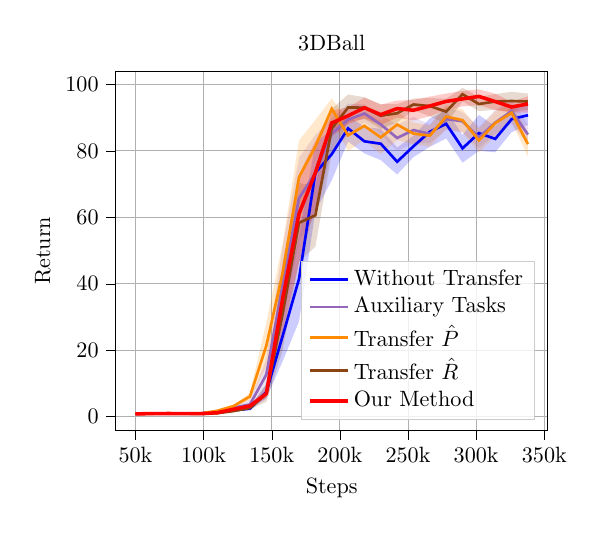
\begin{tikzpicture}[scale=0.8]

\definecolor{color0}{rgb}{0,0,1}
\definecolor{color1}{rgb}{1,0,0}
\definecolor{color2}{rgb}{0.580392156862745,0.403921568627451,0.741176470588235}
\definecolor{color3}{rgb}{1,0.549019607843137,0}
% \definecolor{color4}{rgb}{0.4,0.69803921568,1}
\definecolor{color4}{rgb}{0.55,0.27,0.07}

\begin{axis}[
legend cell align={left},
legend style={
  fill opacity=0.8,
  draw opacity=1,
  text opacity=1,
  at={(0.97,0.03)},
  anchor=south east,
  draw=white!80!black
},
tick align=outside,
tick pos=left,
title={{3DBall}},
scaled ticks=false,
x grid style={white!69.0196078431373!black},
xlabel={{Steps}},
xmajorgrids,
xmin=-14400, xmax=302400,
xtick style={color=black},
% xtick={-50000,0,50000,100000,150000,200000,250000,300000,350000},
% xticklabels={\ensuremath{-}50000,0,50000,100000,150000,200000,250000,300000,350000},
xticklabels={0k,50k,100k,150k,200k,250k,300k,350k},
y grid style={white!69.0196078431373!black},
ylabel={{Return}},
ymajorgrids,
ymin=-4.05404311371744, ymax=103.882906501044,
ytick style={color=black},
ytick={-20,0,20,40,60,80,100,120},
yticklabels={\ensuremath{-}20,0,20,40,60,80,100,120}
]

\path [fill=color0, fill opacity=0.2]
(axis cs:0,0.911586044410865)
--(axis cs:0,0.893576828181744)
--(axis cs:12000,0.950052213847637)
--(axis cs:24000,0.987312424639861)
--(axis cs:36000,0.937743202825387)
--(axis cs:48000,0.98111319377025)
--(axis cs:60000,1.38828979444504)
--(axis cs:72000,1.6821152121226)
--(axis cs:84000,2.09489543334643)
--(axis cs:96000,5.51821187400818)
--(axis cs:108000,16.7050844659805)
--(axis cs:120000,28.6504294724464)
--(axis cs:132000,61.839427675883)
--(axis cs:144000,71.1358873888651)
--(axis cs:156000,82.7840106633504)
--(axis cs:168000,79.247117922465)
--(axis cs:180000,77.2332826207479)
--(axis cs:192000,72.8922494913737)
--(axis cs:204000,78.1251781082153)
--(axis cs:216000,81.2324106190999)
--(axis cs:228000,83.7450485204061)
--(axis cs:240000,76.4509918289185)
--(axis cs:252000,80.0072109603882)
--(axis cs:264000,79.5812978897095)
--(axis cs:276000,85.6326447703044)
--(axis cs:288000,87.8364172744751)
--(axis cs:288000,93.5437296015422)
--(axis cs:288000,93.5437296015422)
--(axis cs:276000,93.296606010437)
--(axis cs:264000,87.377580019633)
--(axis cs:252000,90.8259956512451)
--(axis cs:240000,84.8313724250794)
--(axis cs:228000,92.2400962600708)
--(axis cs:216000,89.7994200897217)
--(axis cs:204000,84.5465452957153)
--(axis cs:192000,81.01156300354)
--(axis cs:180000,86.601208946228)
--(axis cs:168000,87.2577630233765)
--(axis cs:156000,90.4309548492432)
--(axis cs:144000,86.4457708218892)
--(axis cs:132000,82.4021010195414)
--(axis cs:120000,54.4784513861338)
--(axis cs:108000,32.1223968280156)
--(axis cs:96000,9.70910165691376)
--(axis cs:84000,2.72736665960153)
--(axis cs:72000,2.23179793878396)
--(axis cs:60000,1.67258901568254)
--(axis cs:48000,1.04662085551023)
--(axis cs:36000,0.964142741501331)
--(axis cs:24000,1.01115789222717)
--(axis cs:12000,0.972143123229345)
--(axis cs:0,0.911586044410865)
--cycle;



\path [fill=color2, fill opacity=0.2]
(axis cs:0,0.905502462764581)
--(axis cs:0,0.885391654312611)
--(axis cs:12000,0.966521290083726)
--(axis cs:24000,1.00435026784738)
--(axis cs:36000,0.932912302533786)
--(axis cs:48000,0.932445608874162)
--(axis cs:60000,1.26287882602215)
--(axis cs:72000,2.15145396868388)
--(axis cs:84000,2.6549033610026)
--(axis cs:96000,8.27388117281596)
--(axis cs:108000,28.4651692875226)
--(axis cs:120000,52.8148584591548)
--(axis cs:132000,60.6141692867279)
--(axis cs:144000,80.1024012680054)
--(axis cs:156000,84.4604769083659)
--(axis cs:168000,88.4866076533)
--(axis cs:180000,85.0167690658569)
--(axis cs:192000,79.9824682108561)
--(axis cs:204000,82.2037711970011)
--(axis cs:216000,82.2846532465617)
--(axis cs:228000,86.3395181121826)
--(axis cs:240000,85.5953360188802)
--(axis cs:252000,80.8599378534953)
--(axis cs:264000,85.0106308695475)
--(axis cs:276000,88.1110554962158)
--(axis cs:288000,81.7496233393351)
--(axis cs:288000,87.842561726888)
--(axis cs:288000,87.842561726888)
--(axis cs:276000,95.5240037155151)
--(axis cs:264000,92.2460413970947)
--(axis cs:252000,87.2063626505534)
--(axis cs:240000,91.739370241801)
--(axis cs:228000,93.1681739425659)
--(axis cs:216000,87.9079510294596)
--(axis cs:204000,90.2273802439372)
--(axis cs:192000,87.8411529642741)
--(axis cs:180000,90.802943069458)
--(axis cs:168000,93.9773802973429)
--(axis cs:156000,94.2027341613769)
--(axis cs:144000,89.8478268508911)
--(axis cs:132000,84.8754140650431)
--(axis cs:120000,77.9275668433507)
--(axis cs:108000,51.3851270041466)
--(axis cs:96000,17.3506291985512)
--(axis cs:84000,5.12177464898427)
--(axis cs:72000,3.21762132986387)
--(axis cs:60000,1.50324456230799)
--(axis cs:48000,0.984190978348255)
--(axis cs:36000,0.96343360632658)
--(axis cs:24000,1.03399463154872)
--(axis cs:12000,0.99281308277448)
--(axis cs:0,0.905502462764581)
--cycle;

\path [fill=color3, fill opacity=0.2]
(axis cs:0,0.883225904961427)
--(axis cs:0,0.859483804682891)
--(axis cs:12000,0.943223104178905)
--(axis cs:24000,0.969433712323507)
--(axis cs:36000,0.92955630671978)
--(axis cs:48000,0.951388427535693)
--(axis cs:60000,1.62061495105426)
--(axis cs:72000,2.8163078562816)
--(axis cs:84000,5.05053282674154)
--(axis cs:96000,15.0860100111961)
--(axis cs:108000,34.3169784334501)
--(axis cs:120000,59.097813469251)
--(axis cs:132000,72.5467786814372)
--(axis cs:144000,89.129275255839)
--(axis cs:156000,79.964326944987)
--(axis cs:168000,83.2830441665649)
--(axis cs:180000,78.9848361422221)
--(axis cs:192000,83.2655541788737)
--(axis cs:204000,81.9271672312419)
--(axis cs:216000,81.2018585179647)
--(axis cs:228000,86.6242374827067)
--(axis cs:240000,85.5693049367269)
--(axis cs:252000,79.4840527801514)
--(axis cs:264000,84.4132767105103)
--(axis cs:276000,88.8119815724691)
--(axis cs:288000,78.2512013880412)
--(axis cs:288000,85.3612252756755)
--(axis cs:288000,85.3612252756755)
--(axis cs:276000,94.190894955953)
--(axis cs:264000,91.9075223083496)
--(axis cs:252000,86.6295628356934)
--(axis cs:240000,92.5088448435466)
--(axis cs:228000,93.7518971964518)
--(axis cs:216000,87.6470216929118)
--(axis cs:204000,88.5242448628744)
--(axis cs:192000,91.7699772796631)
--(axis cs:180000,89.1489678777059)
--(axis cs:168000,91.7363477834066)
--(axis cs:156000,89.1528789812724)
--(axis cs:144000,95.7775318094889)
--(axis cs:132000,89.3075712280273)
--(axis cs:120000,83.1186680908203)
--(axis cs:108000,52.1497931283315)
--(axis cs:96000,28.3462480015755)
--(axis cs:84000,7.12110461870829)
--(axis cs:72000,3.57770788594087)
--(axis cs:60000,1.94961797014872)
--(axis cs:48000,1.01305635631084)
--(axis cs:36000,0.946282773633798)
--(axis cs:24000,0.990201221803824)
--(axis cs:12000,0.96629344367981)
--(axis cs:0,0.883225904961427)
--cycle;

\path [fill=color4, fill opacity=0.2]
(axis cs:0,0.88139027150472)
--(axis cs:0,0.86060740228494)
--(axis cs:12000,0.897389663040638)
--(axis cs:24000,0.978434031466643)
--(axis cs:36000,0.92770034134388)
--(axis cs:48000,0.852181868771712)
--(axis cs:60000,0.981657914261023)
--(axis cs:72000,1.54076967740059)
--(axis cs:84000,2.2723570318222)
--(axis cs:96000,4.44641343259811)
--(axis cs:108000,20.0529719130993)
--(axis cs:120000,46.6824677054087)
--(axis cs:132000,51.1384569028219)
--(axis cs:144000,79.3364067014058)
--(axis cs:156000,88.6471265767415)
--(axis cs:168000,89.6331681696574)
--(axis cs:180000,86.6542479527791)
--(axis cs:192000,88.5627005742391)
--(axis cs:204000,92.2642791213989)
--(axis cs:216000,90.4127185821533)
--(axis cs:228000,88.1311870473226)
--(axis cs:240000,94.8828336079915)
--(axis cs:252000,91.9616381352742)
--(axis cs:264000,92.361337735494)
--(axis cs:276000,91.751135559082)
--(axis cs:288000,92.3945277201335)
--(axis cs:288000,97.2609303792318)
--(axis cs:288000,97.2609303792318)
--(axis cs:276000,97.8016079406738)
--(axis cs:264000,97.0839737141927)
--(axis cs:252000,96.2726387481689)
--(axis cs:240000,98.9766815185547)
--(axis cs:228000,95.7259859466553)
--(axis cs:216000,95.8932098693848)
--(axis cs:204000,95.7680113601685)
--(axis cs:192000,94.0881837514241)
--(axis cs:180000,94.0629704818726)
--(axis cs:168000,96.1677467880249)
--(axis cs:156000,96.9878536148071)
--(axis cs:144000,92.5953575236003)
--(axis cs:132000,69.496928565979)
--(axis cs:120000,70.3417202097575)
--(axis cs:108000,43.95457969745)
--(axis cs:96000,9.91770686904589)
--(axis cs:84000,3.00842940425873)
--(axis cs:72000,1.85459575299422)
--(axis cs:60000,1.12380301326513)
--(axis cs:48000,0.874550246298313)
--(axis cs:36000,0.966980618814627)
--(axis cs:24000,0.996892310341199)
--(axis cs:12000,0.925474374175072)
--(axis cs:0,0.88139027150472)
--cycle;

\path [fill=color1, fill opacity=0.2]
(axis cs:0,0.871857167919477)
--(axis cs:0,0.860776517748833)
--(axis cs:12000,0.914289421141148)
--(axis cs:24000,0.95932713073492)
--(axis cs:36000,0.921242848654588)
--(axis cs:48000,0.889719801882903)
--(axis cs:60000,1.11461558610201)
--(axis cs:72000,2.03723392283916)
--(axis cs:84000,2.74784810765584)
--(axis cs:96000,5.64052388978005)
--(axis cs:108000,25.4286829140981)
--(axis cs:120000,46.3380833806197)
--(axis cs:132000,62.919475666364)
--(axis cs:144000,84.2873067881266)
--(axis cs:156000,88.0819868774414)
--(axis cs:168000,89.7528482055664)
--(axis cs:180000,87.7862248484294)
--(axis cs:192000,90.0258816553752)
--(axis cs:204000,89.1812913309733)
--(axis cs:216000,90.3935373102824)
--(axis cs:228000,92.2884673461914)
--(axis cs:240000,93.388493057251)
--(axis cs:252000,93.7499954223633)
--(axis cs:264000,92.2617032750448)
--(axis cs:276000,91.5755005340576)
--(axis cs:288000,91.516523958842)
--(axis cs:288000,96.4274523620605)
--(axis cs:288000,96.4274523620605)
--(axis cs:276000,94.7065149205526)
--(axis cs:264000,97.2292050933838)
--(axis cs:252000,98.5404088567098)
--(axis cs:240000,98.0282959187825)
--(axis cs:228000,97.2676238708496)
--(axis cs:216000,96.3480383758545)
--(axis cs:204000,95.355135093689)
--(axis cs:192000,95.1367835184733)
--(axis cs:180000,93.917110748291)
--(axis cs:168000,96.0188167114258)
--(axis cs:156000,93.0501984481811)
--(axis cs:144000,92.1519879277547)
--(axis cs:132000,82.9547321907679)
--(axis cs:120000,72.8582103347778)
--(axis cs:108000,46.2636419054667)
--(axis cs:96000,8.23124446709951)
--(axis cs:84000,3.76994888810317)
--(axis cs:72000,2.49293602403005)
--(axis cs:60000,1.29158747235934)
--(axis cs:48000,0.923121931711833)
--(axis cs:36000,0.942605700612068)
--(axis cs:24000,0.975823855757713)
--(axis cs:12000,0.930647446235021)
--(axis cs:0,0.871857167919477)
--cycle;
\addplot [very thick, color0]
table {%
0 0.901905838777622
12000 0.962037223396699
24000 0.999146792906523
36000 0.951815141230822
48000 1.01409313456416
60000 1.52559088852008
72000 1.94680462131103
84000 2.40893825781345
96000 7.38685420749982
108000 24.3069916057189
120000 41.4718132746061
132000 73.4398098092397
144000 78.9852495770772
156000 86.7667355789185
168000 82.8747308479309
180000 82.1588153673808
192000 76.738635986201
204000 81.3939222195943
216000 85.7553117299398
228000 88.1452280423482
240000 80.7764732204437
252000 85.3530803944906
264000 83.6140804400126
276000 89.553214999644
288000 90.7340763198852
};
\addlegendentry{Without Transfer}

\addplot [very thick, color2]
table {%
0 0.895802424434821
12000 0.979414781109492
24000 1.01822760201891
36000 0.948577052050829
48000 0.958733204432329
60000 1.37656532059113
72000 2.69477556509972
84000 3.70319500122468
96000 12.681743108209
108000 39.698486129268
120000 65.7639903133074
132000 73.354210416158
144000 85.2202657460531
156000 89.3859767936707
168000 91.2461878267924
180000 87.9476788393656
192000 83.8790335863749
204000 86.2696961906433
216000 85.1066269032796
228000 89.6051114163717
240000 88.9006399584452
252000 84.0515214922587
264000 88.5175182601929
276000 91.9629084582011
288000 84.9264506701151
};
\addlegendentry{Auxiliary Tasks}
\addplot [very thick, color3]
table {%
0 0.87093829579552
12000 0.954461890629927
24000 0.979961372739077
36000 0.937324230092764
48000 0.981206701046228
60000 1.7854477313598
72000 3.20104330263138
84000 6.1046913353761
96000 21.3634891139507
108000 43.327407117637
120000 72.0688820735614
132000 81.3282992485682
144000 92.6493984835307
156000 84.6867981441498
168000 87.5211837226868
180000 84.0500229882558
192000 87.9100887560527
204000 85.2127063667297
216000 84.5571378092448
228000 90.3248475883484
240000 89.2384677899679
252000 83.1312809277852
264000 88.3535327097575
276000 91.4740384435018
288000 82.0333514373779
};
\addlegendentry{Transfer $\hat{P}$}
\addplot [very thick, color4]
table {%
0 0.870934468992551
12000 0.91124678465724
24000 0.987519289684296
36000 0.946019084688028
48000 0.862140349630515
60000 1.04412622292638
72000 1.69992994931539
84000 2.62818058981101
96000 6.86198756399155
108000 31.0493813880126
120000 58.3522651816686
132000 60.6335226650238
144000 86.6576751715342
156000 93.0558447364807
168000 93.0219746119181
180000 90.563238965861
192000 91.3316284627279
204000 93.9608005152384
216000 93.4840740112305
228000 91.8142399416606
240000 97.0505021827698
252000 94.1016805768331
264000 94.8691317276001
276000 95.0102150054932
288000 94.8567907740275
};
\addlegendentry{Transfer $\hat{R}$}

\addplot [ultra thick, color1]
table {%
0 0.866553709467252
12000 0.923119978447755
24000 0.967357336485386
36000 0.931596616234382
48000 0.906495008933544
60000 1.20265740027428
72000 2.25544934192499
84000 3.25691274438302
96000 6.92106072714329
108000 35.5233276727041
120000 61.0897104690393
132000 73.4303872014682
144000 88.4033905367533
156000 90.5667071271261
168000 92.9890858202616
180000 90.9145073636373
192000 92.7364072451274
204000 92.2308878267924
216000 93.5267481755574
228000 94.9024087539673
240000 95.6501070798238
252000 96.3939725914001
264000 94.8362269927978
276000 93.2026348889669
288000 94.1352893002828
};
\addlegendentry{Our Method}
\end{axis}

\end{tikzpicture}
 
 \end{subfigure}
 \vspace{-2em}
 \caption{\small{Ablation study of our method on different transferred components.}}
\label{fig:mujoco_ablation}
\end{figure}

\newpage 
\begin{wrapfigure}{r}{0.5\textwidth}
    \centering
    % This file was created with tikzplotlib v0.9.12.
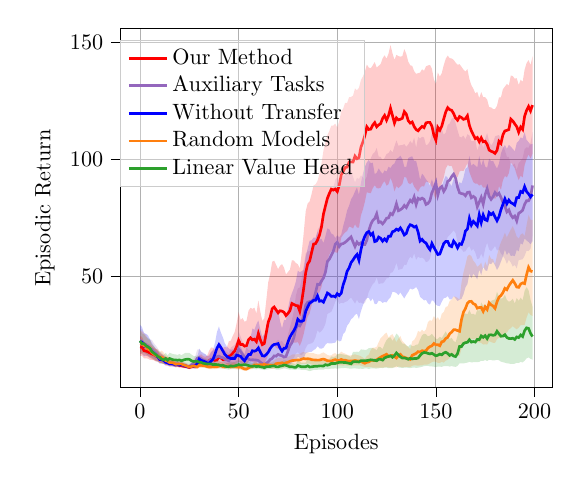
\begin{tikzpicture}[scale=0.8]

\definecolor{color0}{rgb}{0,0,1}
\definecolor{color1}{rgb}{0.580392156862745,0.403921568627451,0.741176470588235}
\definecolor{color2}{rgb}{0.172549019607843,0.627450980392157,0.172549019607843}
\definecolor{color3}{rgb}{1,0.498039215686275,0.0549019607843137}
\definecolor{color4}{rgb}{1,0,0}

% \definecolor{color0}{rgb}{0.12156862745098,0.466666666666667,0.705882352941177}
% \definecolor{color1}{rgb}{1,0.498039215686275,0.0549019607843137}
% \definecolor{color2}{rgb}{0.172549019607843,0.627450980392157,0.172549019607843}
% \definecolor{color3}{rgb}{0.83921568627451,0.152941176470588,0.156862745098039}
% \definecolor{color4}{rgb}{0.580392156862745,0.403921568627451,0.741176470588235}

\begin{axis}[
legend cell align={left},
legend style={
  fill opacity=0.3,
  draw opacity=1,
  text opacity=1,
  at={(0.0,0.97)},
  anchor=north west,
  draw=white!80!black
},
tick align=outside,
tick pos=left,
x grid style={white!69.0196078431373!black},
xmajorgrids,
xmin=-9.95, xmax=208.95,
xtick style={color=black},
xlabel={Episodes},
y grid style={white!69.0196078431373!black},
ymajorgrids,
ymin=2.40030308853674, ymax=155.735241728585,
ytick style={color=black},
ylabel={Episodic Return},
]
\path [fill=color0, fill opacity=0.2]
(axis cs:0,29.2013333333333)
--(axis cs:0,16.666)
--(axis cs:1,16.746)
--(axis cs:2,15.7367333333333)
--(axis cs:3,15.9492533333333)
--(axis cs:4,15.832536)
--(axis cs:5,15.1126288)
--(axis cs:6,14.7700363733333)
--(axis cs:7,14.2426957653333)
--(axis cs:8,13.5740899456)
--(axis cs:9,13.4725386231467)
--(axis cs:10,12.5313642318507)
--(axis cs:11,12.6184247188139)
--(axis cs:12,12.4214064417178)
--(axis cs:13,11.7704584867075)
--(axis cs:14,11.6630334560327)
--(axis cs:15,11.3037600981595)
--(axis cs:16,11.3763414118609)
--(axis cs:17,11.3143397961554)
--(axis cs:18,11.0448051702577)
--(axis cs:19,11.2225108028728)
--(axis cs:20,11.0180086422982)
--(axis cs:21,11.1544069138386)
--(axis cs:22,10.8568588644042)
--(axis cs:23,10.7588204248567)
--(axis cs:24,10.4670563398854)
--(axis cs:25,10.4069784052416)
--(axis cs:26,10.5589160575266)
--(axis cs:27,10.600399512688)
--(axis cs:28,10.406986276817)
--(axis cs:29,10.6521890214536)
--(axis cs:30,11.3416845504962)
--(axis cs:31,11.2400143070637)
--(axis cs:32,11.2252781123176)
--(axis cs:33,11.0935558231874)
--(axis cs:34,10.7748446585499)
--(axis cs:35,10.6532090601733)
--(axis cs:36,10.835900581472)
--(axis cs:37,11.5819871318442)
--(axis cs:38,12.9717897054754)
--(axis cs:39,14.0770317643803)
--(axis cs:40,14.7682254115042)
--(axis cs:41,14.5278469958701)
--(axis cs:42,13.5956109300294)
--(axis cs:43,12.8431554106902)
--(axis cs:44,12.3478576618855)
--(axis cs:45,12.0448861295084)
--(axis cs:46,11.86244223694)
--(axis cs:47,11.7566204562187)
--(axis cs:48,11.8719630316416)
--(axis cs:49,12.3971704253133)
--(axis cs:50,12.4510030069173)
--(axis cs:51,12.4739357388672)
--(axis cs:52,12.0057485910937)
--(axis cs:53,11.6578655395417)
--(axis cs:54,11.6660257649667)
--(axis cs:55,11.5726206119733)
--(axis cs:56,11.2379631562453)
--(axis cs:57,11.5499705249963)
--(axis cs:58,11.519776419997)
--(axis cs:59,11.3490211359976)
--(axis cs:60,11.7122835754648)
--(axis cs:61,11.2564935270385)
--(axis cs:62,10.8451948216308)
--(axis cs:63,10.289489190638)
--(axis cs:64,10.544058019177)
--(axis cs:65,10.9885130820083)
--(axis cs:66,11.2374104656066)
--(axis cs:67,11.7498617058186)
--(axis cs:68,11.7731560313216)
--(axis cs:69,11.6584581583906)
--(axis cs:70,11.9997665267125)
--(axis cs:71,11.73301322137)
--(axis cs:72,11.4530772437627)
--(axis cs:73,11.3891284616768)
--(axis cs:74,11.3775694360081)
--(axis cs:75,11.8151222154731)
--(axis cs:76,12.1373644390452)
--(axis cs:77,12.9364915512361)
--(axis cs:78,13.3689265743223)
--(axis cs:79,13.9350079261245)
--(axis cs:80,15.5342730075662)
--(axis cs:81,15.0404850727197)
--(axis cs:82,14.5989880581757)
--(axis cs:83,14.7723237798739)
--(axis cs:84,16.9965256905658)
--(axis cs:85,17.3896872191193)
--(axis cs:86,17.6382164419621)
--(axis cs:87,17.650506486903)
--(axis cs:88,18.3521385228557)
--(axis cs:89,18.8347108182846)
--(axis cs:90,20.054301987961)
--(axis cs:91,19.1298415903688)
--(axis cs:92,18.9362732722951)
--(axis cs:93,19.3687519511694)
--(axis cs:94,20.6348682276022)
--(axis cs:95,21.4407612487484)
--(axis cs:96,21.1857423323321)
--(axis cs:97,21.1884605325323)
--(axis cs:98,21.4240350926925)
--(axis cs:99,21.5324947408207)
--(axis cs:100,22.9125291259899)
--(axis cs:101,22.0827566341252)
--(axis cs:102,22.3318719739669)
--(axis cs:103,25.2166975791735)
--(axis cs:104,26.1396247300055)
--(axis cs:105,28.784966450671)
--(axis cs:106,29.8735731605368)
--(axis cs:107,31.5652585284295)
--(axis cs:108,32.2320068227436)
--(axis cs:109,33.4519387915282)
--(axis cs:110,33.9475510332225)
--(axis cs:111,31.6179741599114)
--(axis cs:112,34.9673793279291)
--(axis cs:113,37.4738367956766)
--(axis cs:114,39.5381361032079)
--(axis cs:115,40.6302422158997)
--(axis cs:116,40.6824604393864)
--(axis cs:117,39.2254350181758)
--(axis cs:118,40.480281347874)
--(axis cs:119,37.9772250782992)
--(axis cs:120,38.0949133959727)
--(axis cs:121,39.5291307167781)
--(axis cs:122,39.2765712400892)
--(axis cs:123,38.527723658738)
--(axis cs:124,38.9619122603237)
--(axis cs:125,38.7552631415923)
--(axis cs:126,40.0428771799405)
--(axis cs:127,40.9140350772858)
--(axis cs:128,43.2628947284953)
--(axis cs:129,43.1831157827962)
--(axis cs:130,42.7324259595703)
--(axis cs:131,41.8516074343229)
--(axis cs:132,42.9798192807917)
--(axis cs:133,41.6696554246333)
--(axis cs:134,40.4355910063733)
--(axis cs:135,41.9751394717653)
--(axis cs:136,43.2127782440789)
--(axis cs:137,44.7556225952631)
--(axis cs:138,44.2574980762105)
--(axis cs:139,44.6519984609684)
--(axis cs:140,45.3343987687747)
--(axis cs:141,43.9933856816864)
--(axis cs:142,41.1009752120158)
--(axis cs:143,40.4073801696127)
--(axis cs:144,39.5656374690235)
--(axis cs:145,39.8589766418854)
--(axis cs:146,38.3203146468417)
--(axis cs:147,37.8217850508067)
--(axis cs:148,39.757094707312)
--(axis cs:149,39.1778090991829)
--(axis cs:150,37.7483806126797)
--(axis cs:151,37.2907044901437)
--(axis cs:152,37.165763592115)
--(axis cs:153,39.051810873692)
--(axis cs:154,40.5275820322869)
--(axis cs:155,40.7408656258295)
--(axis cs:156,41.4590925006636)
--(axis cs:157,40.0404740005309)
--(axis cs:158,40.0255792004247)
--(axis cs:159,41.3931300270064)
--(axis cs:160,40.4729706882718)
--(axis cs:161,39.3515098839508)
--(axis cs:162,39.938341240494)
--(axis cs:163,40.2629396590618)
--(axis cs:164,42.1631517272495)
--(axis cs:165,45.1747880484662)
--(axis cs:166,46.5794971054397)
--(axis cs:167,51.0423310176851)
--(axis cs:168,49.0535314808147)
--(axis cs:169,51.0082918513184)
--(axis cs:170,49.9593668143881)
--(axis cs:171,48.5469601181771)
--(axis cs:172,52.7840347612084)
--(axis cs:173,50.4068944756334)
--(axis cs:174,53.8651155805067)
--(axis cs:175,52.5052924644053)
--(axis cs:176,52.1837673048576)
--(axis cs:177,55.4326805105528)
--(axis cs:178,55.1522110751089)
--(axis cs:179,56.1015688600871)
--(axis cs:180,54.5605217547363)
--(axis cs:181,52.6216174037891)
--(axis cs:182,54.0366272563646)
--(axis cs:183,56.2023018050917)
--(axis cs:184,58.4006414440733)
--(axis cs:185,61.3403798219253)
--(axis cs:186,59.0385038575403)
--(axis cs:187,60.2706030860322)
--(axis cs:188,58.6088824688258)
--(axis cs:189,58.7665726417273)
--(axis cs:190,58.5397914467152)
--(axis cs:191,61.1713664907055)
--(axis cs:192,60.6146265258977)
--(axis cs:193,64.0513012207182)
--(axis cs:194,63.4876409765745)
--(axis cs:195,66.0965794479263)
--(axis cs:196,65.2169968916744)
--(axis cs:197,64.5660641800062)
--(axis cs:198,63.6656513440049)
--(axis cs:199,64.8849210752039)
--(axis cs:199,106.567226509921)
--(axis cs:199,106.567226509921)
--(axis cs:198,106.183949804068)
--(axis cs:197,107.278353921752)
--(axis cs:196,108.19794240219)
--(axis cs:195,111.546344669404)
--(axis cs:194,108.840930836755)
--(axis cs:193,109.275830212611)
--(axis cs:192,107.768871099097)
--(axis cs:191,106.902672207204)
--(axis cs:190,103.320006925672)
--(axis cs:189,104.414841990423)
--(axis cs:188,105.284052488029)
--(axis cs:187,106.14489894337)
--(axis cs:186,104.371540345879)
--(axis cs:185,106.047675432348)
--(axis cs:184,104.683760957102)
--(axis cs:183,102.429201196378)
--(axis cs:182,98.093751495472)
--(axis cs:181,95.95868936934)
--(axis cs:180,97.5129450450083)
--(axis cs:179,99.2817646395937)
--(axis cs:178,99.0847057994922)
--(axis cs:177,100.212965582699)
--(axis cs:176,96.3074569783732)
--(axis cs:175,96.8081545562998)
--(axis cs:174,99.9341931953747)
--(axis cs:173,97.0906581608851)
--(axis cs:172,101.44640603444)
--(axis cs:171,96.4990075430496)
--(axis cs:170,97.2625927621453)
--(axis cs:169,98.0276576193483)
--(axis cs:168,97.1065720241854)
--(axis cs:167,101.390631696898)
--(axis cs:166,96.4960396211231)
--(axis cs:165,95.8530495264038)
--(axis cs:164,92.0820619080048)
--(axis cs:163,89.533827385006)
--(axis cs:162,90.1755342312574)
--(axis cs:161,88.0690011224051)
--(axis cs:160,90.4022514030064)
--(axis cs:159,91.6258975870914)
--(axis cs:158,88.4067886505309)
--(axis cs:157,89.7331524798303)
--(axis cs:156,91.9994405997878)
--(axis cs:155,92.8485507497348)
--(axis cs:154,90.8264384371684)
--(axis cs:153,88.0162147131272)
--(axis cs:152,85.2101850580757)
--(axis cs:151,84.4589813225946)
--(axis cs:150,87.33039331991)
--(axis cs:149,88.6296583165541)
--(axis cs:148,91.428406229026)
--(axis cs:147,88.6516744529492)
--(axis cs:146,90.3543430661864)
--(axis cs:145,91.3325954993997)
--(axis cs:144,92.7811610409163)
--(axis cs:143,93.8258679678121)
--(axis cs:142,91.2223349597651)
--(axis cs:141,95.7359186997063)
--(axis cs:140,99.2108983746329)
--(axis cs:139,99.2955396349578)
--(axis cs:138,101.209924543697)
--(axis cs:137,100.945655679622)
--(axis cs:136,100.44765293286)
--(axis cs:135,96.7256494994087)
--(axis cs:134,96.7069785409275)
--(axis cs:133,100.041639842826)
--(axis cs:132,101.451299803533)
--(axis cs:131,100.613958087749)
--(axis cs:130,100.124864276353)
--(axis cs:129,98.1143303454412)
--(axis cs:128,97.5584129318015)
--(axis cs:127,96.1805994980853)
--(axis cs:126,96.7503327059399)
--(axis cs:125,94.6794158824249)
--(axis cs:124,95.2046031863645)
--(axis cs:123,93.6792539829556)
--(axis cs:122,94.7139841453612)
--(axis cs:121,96.0334801817014)
--(axis cs:120,94.1414335604601)
--(axis cs:119,93.6164586172418)
--(axis cs:118,98.4703232715523)
--(axis cs:117,98.2182374227737)
--(axis cs:116,99.8056301118005)
--(axis cs:115,98.5730376397506)
--(axis cs:114,96.7491303830216)
--(axis cs:113,93.759912978777)
--(axis cs:112,89.7941412234712)
--(axis cs:111,84.7755931960057)
--(axis cs:110,87.9009914950071)
--(axis cs:109,86.2334893687589)
--(axis cs:108,84.2080283776152)
--(axis cs:107,82.8498688053524)
--(axis cs:106,80.0620026733572)
--(axis cs:105,78.0938366750298)
--(axis cs:104,74.4650458437873)
--(axis cs:103,71.3540573047342)
--(axis cs:102,67.715404964251)
--(axis cs:101,66.6108395386471)
--(axis cs:100,67.4193827566422)
--(axis cs:99,66.2477284458028)
--(axis cs:98,67.7679938905869)
--(axis cs:97,68.1681590299003)
--(axis cs:96,69.943115454042)
--(axis cs:95,70.4033109842191)
--(axis cs:94,67.0286387302739)
--(axis cs:93,64.1171317461757)
--(axis cs:92,65.937998016053)
--(axis cs:91,65.5881641867329)
--(axis cs:90,69.0665385667495)
--(axis cs:89,66.3320898751035)
--(axis cs:88,66.4982790105461)
--(axis cs:87,65.2548487631826)
--(axis cs:86,65.1503109539782)
--(axis cs:85,61.9036386924728)
--(axis cs:84,58.103298365591)
--(axis cs:83,52.7447062903221)
--(axis cs:82,52.088466196236)
--(axis cs:81,51.6596660786283)
--(axis cs:80,52.340999264952)
--(axis cs:79,47.6673324145234)
--(axis cs:78,44.8330821848209)
--(axis cs:77,42.6745193976928)
--(axis cs:76,40.234649247116)
--(axis cs:75,36.0173948922283)
--(axis cs:74,31.1048269486187)
--(axis cs:73,31.2555336857734)
--(axis cs:72,27.6691671072167)
--(axis cs:71,30.6697922173542)
--(axis cs:70,35.2455736050261)
--(axis cs:69,35.946550339616)
--(axis cs:68,35.85768792452)
--(axis cs:67,33.8380265723166)
--(axis cs:66,32.3723665487291)
--(axis cs:65,28.572124852578)
--(axis cs:64,25.9815727323892)
--(axis cs:63,25.2434659154865)
--(axis cs:62,23.9043323943581)
--(axis cs:61,27.1470821596144)
--(axis cs:60,31.0505193661846)
--(axis cs:59,29.3683158743974)
--(axis cs:58,27.0183948429968)
--(axis cs:57,27.6060768870793)
--(axis cs:56,23.5742627755158)
--(axis cs:55,23.2510784693948)
--(axis cs:54,19.9797647534101)
--(axis cs:53,16.5494559417627)
--(axis cs:52,17.95348659387)
--(axis cs:51,19.7918582423375)
--(axis cs:50,20.4564061362552)
--(axis cs:49,21.045007670319)
--(axis cs:48,18.4727595878988)
--(axis cs:47,18.6657828182068)
--(axis cs:46,18.4655618560918)
--(axis cs:45,19.0817856534481)
--(axis cs:44,19.9354820668101)
--(axis cs:43,21.2693525835127)
--(axis cs:42,23.8200240627242)
--(axis cs:41,25.8332800784052)
--(axis cs:40,28.4665167646732)
--(axis cs:39,26.0575626225081)
--(axis cs:38,21.4416199448018)
--(axis cs:37,18.343691597669)
--(axis cs:36,17.4295311637529)
--(axis cs:35,15.7450806213578)
--(axis cs:34,15.7974341100305)
--(axis cs:33,16.6467093042048)
--(axis cs:32,17.2667199635894)
--(axis cs:31,17.6416499544867)
--(axis cs:30,19.0020624431084)
--(axis cs:29,15.0940780538855)
--(axis cs:28,12.6833475673569)
--(axis cs:27,12.8625177925295)
--(axis cs:26,12.4280639073285)
--(axis cs:25,12.084913217494)
--(axis cs:24,12.1144748552008)
--(axis cs:23,12.6097602356676)
--(axis cs:22,12.9121169612512)
--(axis cs:21,13.490146201564)
--(axis cs:20,12.9710160852884)
--(axis cs:19,13.3221034399438)
--(axis cs:18,13.1941292999297)
--(axis cs:17,13.5175782915788)
--(axis cs:16,13.7303061978068)
--(axis cs:15,13.8544660805919)
--(axis cs:14,14.3929992674065)
--(axis cs:13,14.8079157509248)
--(axis cs:12,15.8932280219894)
--(axis cs:11,16.1915350274867)
--(axis cs:10,16.5227521176917)
--(axis cs:9,18.111773480448)
--(axis cs:8,18.87296685056)
--(axis cs:7,20.0412085632)
--(axis cs:6,21.509760704)
--(axis cs:5,23.0871175466667)
--(axis cs:4,24.7503136)
--(axis cs:3,25.2877253333333)
--(axis cs:2,25.62624)
--(axis cs:1,28.2078)
--(axis cs:0,29.2013333333333)
--cycle;



\path [fill=color2, fill opacity=0.2]
(axis cs:0,27.3336666666667)
--(axis cs:0,17.6663333333333)
--(axis cs:1,17.0396666666667)
--(axis cs:2,17.3517333333333)
--(axis cs:3,16.6746533333333)
--(axis cs:4,16.1929226666667)
--(axis cs:5,16.0143381333333)
--(axis cs:6,15.0114705066667)
--(axis cs:7,14.5225097386667)
--(axis cs:8,14.0979411242667)
--(axis cs:9,13.39161956608)
--(axis cs:10,13.2666289861973)
--(axis cs:11,12.5865698556245)
--(axis cs:12,12.382589217833)
--(axis cs:13,12.7794047075997)
--(axis cs:14,12.2301904327464)
--(axis cs:15,12.6573523461971)
--(axis cs:16,12.3190818769577)
--(axis cs:17,12.1085988348995)
--(axis cs:18,12.1935457345863)
--(axis cs:19,12.0547032543357)
--(axis cs:20,11.9904292701352)
--(axis cs:21,11.7656100827748)
--(axis cs:22,12.0124880662199)
--(axis cs:23,12.0965904529759)
--(axis cs:24,12.2839390290474)
--(axis cs:25,12.2071512232379)
--(axis cs:26,11.7656543119237)
--(axis cs:27,11.5858567828723)
--(axis cs:28,11.7753520929645)
--(axis cs:29,11.6602816743716)
--(axis cs:30,11.3548253394973)
--(axis cs:31,11.2570602715978)
--(axis cs:32,10.9922482172782)
--(axis cs:33,10.7803985738226)
--(axis cs:34,10.7643188590581)
--(axis cs:35,10.8113884205798)
--(axis cs:36,10.8823774031305)
--(axis cs:37,10.6592352558377)
--(axis cs:38,10.8407215380035)
--(axis cs:39,10.7125772304028)
--(axis cs:40,10.7100617843223)
--(axis cs:41,10.5280494274578)
--(axis cs:42,10.5891062086329)
--(axis cs:43,10.3446183002397)
--(axis cs:44,10.1756279735251)
--(axis cs:45,10.0138357121534)
--(axis cs:46,10.271001903056)
--(axis cs:47,10.1968015224448)
--(axis cs:48,10.3974412179559)
--(axis cs:49,10.431286307698)
--(axis cs:50,10.7516957128251)
--(axis cs:51,10.6012232369267)
--(axis cs:52,10.6009785895414)
--(axis cs:53,10.6607162049664)
--(axis cs:54,10.6485729639732)
--(axis cs:55,10.4655250378452)
--(axis cs:56,10.2057533636095)
--(axis cs:57,10.2712693575543)
--(axis cs:58,10.2970154860434)
--(axis cs:59,10.1376123888347)
--(axis cs:60,10.3299565777344)
--(axis cs:61,10.1306319288542)
--(axis cs:62,10.0444388764167)
--(axis cs:63,9.8354844344667)
--(axis cs:64,10.00165421424)
--(axis cs:65,10.1146567047254)
--(axis cs:66,10.2517253637803)
--(axis cs:67,10.3747136243576)
--(axis cs:68,10.4530375661527)
--(axis cs:69,10.0423633862555)
--(axis cs:70,9.96055737567107)
--(axis cs:71,10.1017125672035)
--(axis cs:72,10.2813033870962)
--(axis cs:73,10.5517093763436)
--(axis cs:74,10.3880341677415)
--(axis cs:75,10.1704273341932)
--(axis cs:76,10.0030085340212)
--(axis cs:77,10.082406827217)
--(axis cs:78,9.95259212844027)
--(axis cs:79,9.94874036941888)
--(axis cs:80,10.1989256288684)
--(axis cs:81,10.0658071697614)
--(axis cs:82,9.8793124024758)
--(axis cs:83,9.89011658864731)
--(axis cs:84,9.90542660425118)
--(axis cs:85,9.63767461673428)
--(axis cs:86,9.37007302672076)
--(axis cs:87,9.6160584213766)
--(axis cs:88,9.86618007043462)
--(axis cs:89,9.95294405634769)
--(axis cs:90,9.94902191174482)
--(axis cs:91,10.0525508627292)
--(axis cs:92,9.96870735685002)
--(axis cs:93,9.96823255214668)
--(axis cs:94,10.3545860417173)
--(axis cs:95,10.1769355000405)
--(axis cs:96,10.3081484000324)
--(axis cs:97,10.4464520533593)
--(axis cs:98,10.4638283093541)
--(axis cs:99,10.5377293141499)
--(axis cs:100,10.4435167846533)
--(axis cs:101,10.5214800943893)
--(axis cs:102,10.6505174088448)
--(axis cs:103,10.6603472604091)
--(axis cs:104,10.7548778083273)
--(axis cs:105,10.6172355799952)
--(axis cs:106,10.5004551306628)
--(axis cs:107,10.3870307711969)
--(axis cs:108,10.5429579502909)
--(axis cs:109,10.6143663602327)
--(axis cs:110,10.4514264215195)
--(axis cs:111,10.3744078038823)
--(axis cs:112,10.4128595764391)
--(axis cs:113,10.316954327818)
--(axis cs:114,10.5468967955877)
--(axis cs:115,10.5441841031368)
--(axis cs:116,10.2752806158428)
--(axis cs:117,10.5333578260076)
--(axis cs:118,10.5666195941394)
--(axis cs:119,10.4932290086448)
--(axis cs:120,10.4612498735825)
--(axis cs:121,10.5755332321994)
--(axis cs:122,10.7604265857595)
--(axis cs:123,10.6883412686076)
--(axis cs:124,10.8772730148861)
--(axis cs:125,10.8884184119089)
--(axis cs:126,10.5970680628604)
--(axis cs:127,10.7037877836217)
--(axis cs:128,10.696296893564)
--(axis cs:129,11.0037041815179)
--(axis cs:130,11.502830011881)
--(axis cs:131,10.9755973428381)
--(axis cs:132,10.8404778742705)
--(axis cs:133,10.7322489660831)
--(axis cs:134,10.8323325061998)
--(axis cs:135,10.9258660049598)
--(axis cs:136,10.7672928039679)
--(axis cs:137,10.6803675765076)
--(axis cs:138,10.8175607278728)
--(axis cs:139,10.9406485822982)
--(axis cs:140,10.7391855325052)
--(axis cs:141,10.8578817593375)
--(axis cs:142,10.99290540747)
--(axis cs:143,11.2409909926427)
--(axis cs:144,11.5061261274475)
--(axis cs:145,11.5847675686246)
--(axis cs:146,11.6344140548997)
--(axis cs:147,11.3807312439198)
--(axis cs:148,11.3777849951358)
--(axis cs:149,11.2688946627753)
--(axis cs:150,11.1017157302203)
--(axis cs:151,11.3345725841762)
--(axis cs:152,11.2809914006743)
--(axis cs:153,11.1980597872061)
--(axis cs:154,11.5315811630982)
--(axis cs:155,11.4917982638119)
--(axis cs:156,11.5600386110495)
--(axis cs:157,11.3080308888396)
--(axis cs:158,11.5596913777384)
--(axis cs:159,11.3144197688574)
--(axis cs:160,11.2048024817526)
--(axis cs:161,11.6169753187354)
--(axis cs:162,12.7333135883216)
--(axis cs:163,12.6796508706573)
--(axis cs:164,12.6301873631925)
--(axis cs:165,12.850749890554)
--(axis cs:166,13.0271999124432)
--(axis cs:167,13.3416265966212)
--(axis cs:168,13.1132346106303)
--(axis cs:169,13.1771210218376)
--(axis cs:170,13.2083634841367)
--(axis cs:171,13.1800241206427)
--(axis cs:172,13.3572859631808)
--(axis cs:173,13.812362103878)
--(axis cs:174,13.7362896831024)
--(axis cs:175,14.1223650798153)
--(axis cs:176,13.7045587305189)
--(axis cs:177,14.2232469844151)
--(axis cs:178,14.1251975875321)
--(axis cs:179,13.913291403359)
--(axis cs:180,14.0171664560205)
--(axis cs:181,14.1935998314831)
--(axis cs:182,14.0148798651865)
--(axis cs:183,13.4249705588158)
--(axis cs:184,13.1731764470527)
--(axis cs:185,12.9984744909755)
--(axis cs:186,12.705446259447)
--(axis cs:187,12.624090340891)
--(axis cs:188,12.4126056060461)
--(axis cs:189,12.4628844848369)
--(axis cs:190,12.5369075878695)
--(axis cs:191,12.9426594036289)
--(axis cs:192,12.8340608562365)
--(axis cs:193,13.3204486849892)
--(axis cs:194,13.0629589479914)
--(axis cs:195,13.8429004917264)
--(axis cs:196,14.8341870600478)
--(axis cs:197,15.2330829813716)
--(axis cs:198,14.6329997184306)
--(axis cs:199,14.2729331080778)
--(axis cs:199,36.9032859631685)
--(axis cs:199,36.9032859631685)
--(axis cs:198,39.8790241206273)
--(axis cs:197,43.9735301507841)
--(axis cs:196,45.2741626884801)
--(axis cs:195,43.6926200272668)
--(axis cs:194,39.6067750340835)
--(axis cs:193,40.790635459271)
--(axis cs:192,39.4212109907554)
--(axis cs:191,40.6257637384443)
--(axis cs:190,38.2897046730553)
--(axis cs:189,40.3198808413192)
--(axis cs:188,39.389101051649)
--(axis cs:187,39.0682096478945)
--(axis cs:186,39.8006787265348)
--(axis cs:185,42.0505984081685)
--(axis cs:184,40.5794146768773)
--(axis cs:183,40.3575183460966)
--(axis cs:182,41.1377312659541)
--(axis cs:181,43.305497415776)
--(axis cs:180,40.08812176972)
--(axis cs:179,39.74115221215)
--(axis cs:178,39.3427735985209)
--(axis cs:177,38.5529669981511)
--(axis cs:176,35.7159587476888)
--(axis cs:175,38.1108651012777)
--(axis cs:174,37.2630813765972)
--(axis cs:173,38.7199350540798)
--(axis cs:172,35.1898354842664)
--(axis cs:171,35.5703776886663)
--(axis cs:170,33.3040554441663)
--(axis cs:169,33.9125693052078)
--(axis cs:168,33.7142949648431)
--(axis cs:167,35.4927853727206)
--(axis cs:166,33.699315049234)
--(axis cs:165,34.0063104782092)
--(axis cs:164,33.8909714310949)
--(axis cs:163,29.8961309555352)
--(axis cs:162,29.7282470277524)
--(axis cs:161,24.4598087846905)
--(axis cs:160,21.6997609808631)
--(axis cs:159,22.2579512260789)
--(axis cs:158,23.6141056992652)
--(axis cs:157,23.0841321240816)
--(axis cs:156,24.6800818217686)
--(axis cs:155,26.3666856105441)
--(axis cs:154,24.9650236798468)
--(axis cs:153,23.4783629331418)
--(axis cs:152,24.0812869997606)
--(axis cs:151,23.1848587497008)
--(axis cs:150,23.1391567704593)
--(axis cs:149,24.2406126297408)
--(axis cs:148,25.317265787176)
--(axis cs:147,24.5630822339699)
--(axis cs:146,24.2703527924624)
--(axis cs:145,25.1377743239114)
--(axis cs:144,25.3635512382225)
--(axis cs:143,24.6870223811115)
--(axis cs:142,22.9411113097227)
--(axis cs:141,20.7845558038201)
--(axis cs:140,20.6638614214418)
--(axis cs:139,20.1795767768022)
--(axis cs:138,19.9827209710028)
--(axis cs:137,20.8116512137534)
--(axis cs:136,19.7975640171918)
--(axis cs:135,20.4134550214898)
--(axis cs:134,21.0918187768622)
--(axis cs:133,21.1897734710777)
--(axis cs:132,22.5538001721805)
--(axis cs:131,24.533833548559)
--(axis cs:130,25.4504586023654)
--(axis cs:129,23.7962399196234)
--(axis cs:128,22.2613832328626)
--(axis cs:127,23.8350623744116)
--(axis cs:126,23.5687446346811)
--(axis cs:125,22.6769307933514)
--(axis cs:124,20.9793301583559)
--(axis cs:123,18.7984126979449)
--(axis cs:122,19.5728492057645)
--(axis cs:121,19.8739781738723)
--(axis cs:120,18.342139384007)
--(axis cs:119,18.8610075633421)
--(axis cs:118,19.2345094541776)
--(axis cs:117,19.2929701510553)
--(axis cs:116,19.1991293554858)
--(axis cs:115,18.5404116943573)
--(axis cs:114,18.4584312846133)
--(axis cs:113,18.5812891057666)
--(axis cs:112,18.6427780488749)
--(axis cs:111,17.5862225610936)
--(axis cs:110,17.6744448680337)
--(axis cs:109,17.5510560850421)
--(axis cs:108,17.6138201063026)
--(axis cs:107,15.4171917995449)
--(axis cs:106,15.8380730827645)
--(axis cs:105,16.1725080201223)
--(axis cs:104,16.2988016918195)
--(axis cs:103,16.5318354481077)
--(axis cs:102,16.6397109768013)
--(axis cs:101,16.8410553876683)
--(axis cs:100,16.5175692345854)
--(axis cs:99,15.5466282098984)
--(axis cs:98,15.4913685957063)
--(axis cs:97,15.6472940779663)
--(axis cs:96,14.5589509307912)
--(axis cs:95,14.1316053301556)
--(axis cs:94,14.4143399960278)
--(axis cs:93,13.6345083283681)
--(axis cs:92,13.8430520771268)
--(axis cs:91,13.7453984297419)
--(axis cs:90,13.6650813705107)
--(axis cs:89,13.6896850464717)
--(axis cs:88,13.6704396414229)
--(axis cs:87,13.7380495517787)
--(axis cs:86,14.03897860639)
--(axis cs:85,14.9653065913208)
--(axis cs:84,12.9649665724844)
--(axis cs:83,13.0059582156055)
--(axis cs:82,12.9404477695069)
--(axis cs:81,13.3255597118836)
--(axis cs:80,13.8736163065211)
--(axis cs:79,12.4252703831514)
--(axis cs:78,12.5815879789393)
--(axis cs:77,12.8517349736741)
--(axis cs:76,12.8395853837592)
--(axis cs:75,13.3911483963657)
--(axis cs:74,13.9306021621238)
--(axis cs:73,14.0215860359881)
--(axis cs:72,13.5436492116518)
--(axis cs:71,13.3462281812314)
--(axis cs:70,12.7572018932059)
--(axis cs:69,12.7880023665074)
--(axis cs:68,13.0933362914676)
--(axis cs:67,12.9915870310012)
--(axis cs:66,12.7559837887515)
--(axis cs:65,12.7864797359394)
--(axis cs:64,12.9829330032575)
--(axis cs:63,12.1618329207386)
--(axis cs:62,12.4437911509232)
--(axis cs:61,12.6379056053207)
--(axis cs:60,12.8390486733175)
--(axis cs:59,12.6904775083136)
--(axis cs:58,13.096346885392)
--(axis cs:57,12.8536002734067)
--(axis cs:56,13.0920003417583)
--(axis cs:55,13.4482504271979)
--(axis cs:54,13.7435630339974)
--(axis cs:53,14.0960371258301)
--(axis cs:52,13.8532964072876)
--(axis cs:51,13.7666205091095)
--(axis cs:50,14.0498589697202)
--(axis cs:49,13.7705737121502)
--(axis cs:48,13.2381338068544)
--(axis cs:47,13.1392505919014)
--(axis cs:46,13.48239657321)
--(axis cs:45,12.9695790498459)
--(axis cs:44,12.7785571456407)
--(axis cs:43,13.0313630987175)
--(axis cs:42,13.5307038733969)
--(axis cs:41,13.3049631750795)
--(axis cs:40,13.697870635516)
--(axis cs:39,13.947338294395)
--(axis cs:38,14.0340062013271)
--(axis cs:37,13.9925077516589)
--(axis cs:36,14.507218022907)
--(axis cs:35,14.5756891953004)
--(axis cs:34,14.6111948274588)
--(axis cs:33,14.8222435343236)
--(axis cs:32,14.9610544179044)
--(axis cs:31,15.5262346890472)
--(axis cs:30,15.6158766946424)
--(axis cs:29,16.1447625349696)
--(axis cs:28,15.705953168712)
--(axis cs:27,15.89069146089)
--(axis cs:26,16.4883643261126)
--(axis cs:25,17.1602054076407)
--(axis cs:24,17.1252567595509)
--(axis cs:23,17.1732376161052)
--(axis cs:22,16.6998803534649)
--(axis cs:21,16.1831837751644)
--(axis cs:20,16.6956463856222)
--(axis cs:19,16.3028079820278)
--(axis cs:18,16.5034266442014)
--(axis cs:17,16.6125333052517)
--(axis cs:16,16.8905832982313)
--(axis cs:15,17.2381457894558)
--(axis cs:14,16.1310155701531)
--(axis cs:13,17.1887694626914)
--(axis cs:12,16.2859618283643)
--(axis cs:11,16.6240356187887)
--(axis cs:10,17.5883778568192)
--(axis cs:9,18.1521389876907)
--(axis cs:8,19.09009040128)
--(axis cs:7,20.0375296682667)
--(axis cs:6,20.788578752)
--(axis cs:5,22.8606401066667)
--(axis cs:4,23.4090501333333)
--(axis cs:3,24.002896)
--(axis cs:2,25.2034533333333)
--(axis cs:1,25.4204)
--(axis cs:0,27.3336666666667)
--cycle;

\path [fill=color3, fill opacity=0.2]
(axis cs:0,26.5346666666667)
--(axis cs:0,16.4656666666667)
--(axis cs:1,16.6256666666667)
--(axis cs:2,16.0870666666667)
--(axis cs:3,16.2429866666667)
--(axis cs:4,15.4943893333333)
--(axis cs:5,15.0487781333333)
--(axis cs:6,14.43215584)
--(axis cs:7,14.0789913386667)
--(axis cs:8,13.5098597376)
--(axis cs:9,13.6077544567467)
--(axis cs:10,12.799470232064)
--(axis cs:11,12.9861095189845)
--(axis cs:12,12.728820948521)
--(axis cs:13,12.1296567588168)
--(axis cs:14,12.0036587403867)
--(axis cs:15,11.5561936589761)
--(axis cs:16,11.5649549271809)
--(axis cs:17,11.425297275078)
--(axis cs:18,11.0469044867291)
--(axis cs:19,11.1508569227166)
--(axis cs:20,11.1006855381733)
--(axis cs:21,11.1805484305386)
--(axis cs:22,10.8710387444309)
--(axis cs:23,10.7568309955447)
--(axis cs:24,10.4854647964358)
--(axis cs:25,10.281705170482)
--(axis cs:26,10.4519641363856)
--(axis cs:27,10.6348379757751)
--(axis cs:28,10.4412037139534)
--(axis cs:29,10.3128963044961)
--(axis cs:30,10.7503170435969)
--(axis cs:31,10.7668536348775)
--(axis cs:32,10.7068162412353)
--(axis cs:33,10.7387863263216)
--(axis cs:34,10.4510290610573)
--(axis cs:35,10.2941565821792)
--(axis cs:36,10.1753252657433)
--(axis cs:37,10.2935268792613)
--(axis cs:38,10.2481548367424)
--(axis cs:39,10.2984572027272)
--(axis cs:40,10.4120324288485)
--(axis cs:41,10.6029592764121)
--(axis cs:42,10.3290340877964)
--(axis cs:43,10.3432272702371)
--(axis cs:44,10.4678484828563)
--(axis cs:45,10.5342787862851)
--(axis cs:46,10.1807563623614)
--(axis cs:47,10.4178717565558)
--(axis cs:48,10.174230738578)
--(axis cs:49,10.0727179241957)
--(axis cs:50,9.90484100602322)
--(axis cs:51,10.0572061381519)
--(axis cs:52,9.70576491052153)
--(axis cs:53,9.47121192841722)
--(axis cs:54,9.47696954273378)
--(axis cs:55,9.80157563418702)
--(axis cs:56,10.274593840683)
--(axis cs:57,10.3596750725464)
--(axis cs:58,10.8477400580371)
--(axis cs:59,10.978125379763)
--(axis cs:60,10.8625003038104)
--(axis cs:61,11.1299335763817)
--(axis cs:62,11.063813527772)
--(axis cs:63,11.2309841555509)
--(axis cs:64,10.9380539911074)
--(axis cs:65,10.7571098595526)
--(axis cs:66,10.5056878876421)
--(axis cs:67,10.3445503101137)
--(axis cs:68,10.3155735814243)
--(axis cs:69,10.9457255318061)
--(axis cs:70,11.0365804254449)
--(axis cs:71,11.0158643403559)
--(axis cs:72,11.0526914722847)
--(axis cs:73,10.7288198444944)
--(axis cs:74,11.0963892089289)
--(axis cs:75,11.3504447004764)
--(axis cs:76,11.7935557603811)
--(axis cs:77,11.8814446083049)
--(axis cs:78,11.9650890199773)
--(axis cs:79,12.2587378826485)
--(axis cs:80,12.1269236394521)
--(axis cs:81,12.201472244895)
--(axis cs:82,12.421177795916)
--(axis cs:83,12.5502755700662)
--(axis cs:84,12.4667537893863)
--(axis cs:85,12.5532696981757)
--(axis cs:86,12.5692824252072)
--(axis cs:87,12.1354259401658)
--(axis cs:88,12.0415407521326)
--(axis cs:89,12.1132326017061)
--(axis cs:90,12.1505860813649)
--(axis cs:91,12.2068688650919)
--(axis cs:92,12.2320950920735)
--(axis cs:93,12.3390094069921)
--(axis cs:94,12.1844741922604)
--(axis cs:95,11.8675793538083)
--(axis cs:96,11.86739681638)
--(axis cs:97,11.7072507864373)
--(axis cs:98,11.9258006291499)
--(axis cs:99,12.0939071699865)
--(axis cs:100,11.8884590693226)
--(axis cs:101,11.7907005887914)
--(axis cs:102,11.8123604710331)
--(axis cs:103,11.7032217101598)
--(axis cs:104,11.8957773681279)
--(axis cs:105,11.7499552278356)
--(axis cs:106,11.6666308489352)
--(axis cs:107,11.7132380124815)
--(axis cs:108,11.7171237433185)
--(axis cs:109,11.8402989946548)
--(axis cs:110,11.7789058623905)
--(axis cs:111,11.8297246899124)
--(axis cs:112,11.7304464185966)
--(axis cs:113,11.4043571348773)
--(axis cs:114,11.2034857079018)
--(axis cs:115,11.2027885663215)
--(axis cs:116,11.1620975197238)
--(axis cs:117,11.2228113491124)
--(axis cs:118,10.9182490792899)
--(axis cs:119,10.8278659300986)
--(axis cs:120,10.9289594107455)
--(axis cs:121,10.8164341952631)
--(axis cs:122,10.8730806895438)
--(axis cs:123,10.8517978849684)
--(axis cs:124,10.974771641308)
--(axis cs:125,11.1064173130464)
--(axis cs:126,10.9184671837705)
--(axis cs:127,10.8613737470164)
--(axis cs:128,10.8755656642798)
--(axis cs:129,10.9936525314238)
--(axis cs:130,10.9281886918057)
--(axis cs:131,11.3290176201112)
--(axis cs:132,11.2164807627557)
--(axis cs:133,11.0064512768712)
--(axis cs:134,11.0718276881636)
--(axis cs:135,11.1440621505309)
--(axis cs:136,11.1352497204247)
--(axis cs:137,11.1281331096731)
--(axis cs:138,11.6557731544052)
--(axis cs:139,11.8712185235241)
--(axis cs:140,11.810241485486)
--(axis cs:141,11.6881265217221)
--(axis cs:142,11.8037678840443)
--(axis cs:143,11.8494143072355)
--(axis cs:144,12.1727314457884)
--(axis cs:145,12.111518489964)
--(axis cs:146,12.2487481253046)
--(axis cs:147,12.725531833577)
--(axis cs:148,13.2266921335283)
--(axis cs:149,13.4813537068226)
--(axis cs:150,13.3117496321247)
--(axis cs:151,12.9027330390331)
--(axis cs:152,12.8687197645598)
--(axis cs:153,13.3748424783145)
--(axis cs:154,12.993007315985)
--(axis cs:155,13.8008725194546)
--(axis cs:156,14.2470980155637)
--(axis cs:157,14.997278412451)
--(axis cs:158,15.6176893966274)
--(axis cs:159,16.1672848506353)
--(axis cs:160,16.3660945471749)
--(axis cs:161,16.0328089710732)
--(axis cs:162,15.8527805101919)
--(axis cs:163,18.8482910748202)
--(axis cs:164,20.3378328598562)
--(axis cs:165,20.8233996212183)
--(axis cs:166,21.9317196969746)
--(axis cs:167,22.9048424242464)
--(axis cs:168,23.1570072727304)
--(axis cs:169,22.9175391515177)
--(axis cs:170,23.0136979878808)
--(axis cs:171,21.7308250569713)
--(axis cs:172,21.697460045577)
--(axis cs:173,21.4176347031283)
--(axis cs:174,20.747241095836)
--(axis cs:175,20.8711262100021)
--(axis cs:176,20.7231676346684)
--(axis cs:177,22.204467441068)
--(axis cs:178,21.8434406195211)
--(axis cs:179,21.4541524956169)
--(axis cs:180,21.4626553298268)
--(axis cs:181,23.0289909305281)
--(axis cs:182,23.6291927444225)
--(axis cs:183,23.5096208622047)
--(axis cs:184,24.0875633564304)
--(axis cs:185,25.602317351811)
--(axis cs:186,25.8281205481155)
--(axis cs:187,27.141363105159)
--(axis cs:188,27.7664238174606)
--(axis cs:189,28.5794057206351)
--(axis cs:190,27.8433245765081)
--(axis cs:191,27.2477929945398)
--(axis cs:192,27.9379010622985)
--(axis cs:193,29.0697875165055)
--(axis cs:194,29.0358300132044)
--(axis cs:195,29.1815973438968)
--(axis cs:196,32.2369445417841)
--(axis cs:197,34.5554889667606)
--(axis cs:198,33.3776578400752)
--(axis cs:199,32.9815262720601)
--(axis cs:199,73.9267964471954)
--(axis cs:199,73.9267964471954)
--(axis cs:198,74.1413288923275)
--(axis cs:197,76.1262444487428)
--(axis cs:196,71.7826388942618)
--(axis cs:195,67.0448819511606)
--(axis cs:194,68.2801024389507)
--(axis cs:193,67.7416280486884)
--(axis cs:192,65.9932017275271)
--(axis cs:191,66.8494188260756)
--(axis cs:190,69.2866901992612)
--(axis cs:189,71.3645294157431)
--(axis cs:188,69.9049951030122)
--(axis cs:187,68.262160545432)
--(axis cs:186,66.4773673484566)
--(axis cs:185,68.5131258522375)
--(axis cs:184,66.3313239819635)
--(axis cs:183,64.4717383107877)
--(axis cs:182,62.0712562218179)
--(axis cs:181,58.8389869439391)
--(axis cs:180,54.8972336799239)
--(axis cs:179,57.2622920999048)
--(axis cs:178,57.376615124881)
--(axis cs:177,59.020685572768)
--(axis cs:176,54.1501902992933)
--(axis cs:175,56.2124878741166)
--(axis cs:174,52.5987765093124)
--(axis cs:173,55.7472206366405)
--(axis cs:172,54.6422757958006)
--(axis cs:171,53.9425947447508)
--(axis cs:170,55.6362434309385)
--(axis cs:169,56.5535542886731)
--(axis cs:168,58.5667761941747)
--(axis cs:167,59.1464702427184)
--(axis cs:166,58.474587803398)
--(axis cs:165,54.8331514209142)
--(axis cs:164,51.5910226094761)
--(axis cs:163,47.1633615951785)
--(axis cs:162,39.8957853273064)
--(axis cs:161,40.694481659133)
--(axis cs:160,41.1664354072496)
--(axis cs:159,41.2909609257286)
--(axis cs:158,39.8860344904941)
--(axis cs:157,39.390626446451)
--(axis cs:156,37.0881997247304)
--(axis cs:155,36.7851663225797)
--(axis cs:154,34.631291236558)
--(axis cs:153,33.9301973790308)
--(axis cs:152,31.0126633904552)
--(axis cs:151,32.4407459047356)
--(axis cs:150,31.5757657142529)
--(axis cs:149,32.9028738094828)
--(axis cs:148,30.8699255951868)
--(axis cs:147,31.1122403273168)
--(axis cs:146,30.3568837424793)
--(axis cs:145,27.2623546780992)
--(axis cs:144,26.2942766809573)
--(axis cs:143,27.0927625178633)
--(axis cs:142,26.0573698139958)
--(axis cs:141,26.5797122674947)
--(axis cs:140,24.0903070010351)
--(axis cs:139,22.7292170846272)
--(axis cs:138,22.1111880224506)
--(axis cs:137,18.8377350280633)
--(axis cs:136,19.6387521184124)
--(axis cs:135,20.3816068146822)
--(axis cs:134,21.4016751850194)
--(axis cs:133,22.2269273146076)
--(axis cs:132,24.3919091432595)
--(axis cs:131,23.2981364290744)
--(axis cs:130,21.7225038696764)
--(axis cs:129,23.4697131704288)
--(axis cs:128,25.162141463036)
--(axis cs:127,24.6108434954617)
--(axis cs:126,23.7218043693271)
--(axis cs:125,25.8605054616589)
--(axis cs:124,25.2251318270736)
--(axis cs:123,24.2225814505086)
--(axis cs:122,23.4615601464691)
--(axis cs:121,21.7349501830864)
--(axis cs:120,19.7431043955247)
--(axis cs:119,19.4037971610725)
--(axis cs:118,19.4456631180073)
--(axis cs:117,18.4486622308425)
--(axis cs:116,16.3941611218864)
--(axis cs:115,15.8592847356913)
--(axis cs:114,14.5734392529475)
--(axis cs:113,15.1751323995177)
--(axis cs:112,15.7105821660638)
--(axis cs:111,16.0714777075798)
--(axis cs:110,16.255930467808)
--(axis cs:109,16.5615797514267)
--(axis cs:108,16.37689135595)
--(axis cs:107,16.0622808616042)
--(axis cs:106,16.1443510770053)
--(axis cs:105,16.3970221795899)
--(axis cs:104,16.8712777244874)
--(axis cs:103,17.1471804889426)
--(axis cs:102,17.7172256111782)
--(axis cs:101,16.6548653473061)
--(axis cs:100,16.401665017466)
--(axis cs:99,17.0519146051658)
--(axis cs:98,16.8063932564573)
--(axis cs:97,16.1329082372383)
--(axis cs:96,16.0244686298812)
--(axis cs:95,16.2805024540181)
--(axis cs:94,16.8838780675227)
--(axis cs:93,17.37976425107)
--(axis cs:92,17.0497053138375)
--(axis cs:91,16.4871316422968)
--(axis cs:90,16.5002478862044)
--(axis cs:89,16.7169765244222)
--(axis cs:88,17.0378873221944)
--(axis cs:87,17.0472758194096)
--(axis cs:86,17.158844774262)
--(axis cs:85,17.4484726344942)
--(axis cs:84,17.2437574597844)
--(axis cs:83,17.5878634913972)
--(axis cs:82,17.3260793642465)
--(axis cs:81,16.6740992053081)
--(axis cs:80,16.7092073399685)
--(axis cs:79,16.4780925082939)
--(axis cs:78,16.5809489687008)
--(axis cs:77,16.434186210876)
--(axis cs:76,15.8009827635949)
--(axis cs:75,15.4761451211603)
--(axis cs:74,15.2201814014504)
--(axis cs:73,14.8251434184797)
--(axis cs:72,15.3060959397663)
--(axis cs:71,15.0408699247079)
--(axis cs:70,15.0010874058848)
--(axis cs:69,14.6510259240227)
--(axis cs:68,13.9385324050284)
--(axis cs:67,13.4312488396188)
--(axis cs:66,13.4973943828569)
--(axis cs:65,13.4962429785711)
--(axis cs:64,13.3452203898805)
--(axis cs:63,13.564858820684)
--(axis cs:62,13.1477401925216)
--(axis cs:61,13.342925240652)
--(axis cs:60,13.003656550815)
--(axis cs:59,13.3879040218521)
--(axis cs:58,13.4182133606485)
--(axis cs:57,12.489350034144)
--(axis cs:56,12.2950208760133)
--(axis cs:55,11.8103594283499)
--(axis cs:54,11.3296159521041)
--(axis cs:53,11.3452699401301)
--(axis cs:52,11.8065040918293)
--(axis cs:51,12.4081301147866)
--(axis cs:50,12.4351626434833)
--(axis cs:49,12.6272033043541)
--(axis cs:48,12.9590041304426)
--(axis cs:47,12.9987551630532)
--(axis cs:46,12.4316939538165)
--(axis cs:45,12.7728674422707)
--(axis cs:44,12.8825843028383)
--(axis cs:43,12.3363970452146)
--(axis cs:42,12.5204129731849)
--(axis cs:41,13.1338495498145)
--(axis cs:40,12.8337286039348)
--(axis cs:39,12.4421607549185)
--(axis cs:38,12.3526176103148)
--(axis cs:37,12.5741053462268)
--(axis cs:36,12.3758816827835)
--(axis cs:35,12.1196854368127)
--(axis cs:34,12.3328567960158)
--(axis cs:33,12.8743209950198)
--(axis cs:32,12.9262345771081)
--(axis cs:31,13.2993765547184)
--(axis cs:30,13.3325540267314)
--(axis cs:29,12.2906925334142)
--(axis cs:28,12.6216990001011)
--(axis cs:27,12.8604570834597)
--(axis cs:26,12.5170713543246)
--(axis cs:25,12.4213391929058)
--(axis cs:24,12.5682573244656)
--(axis cs:23,12.9936549889153)
--(axis cs:22,13.4504020694775)
--(axis cs:21,14.0713359201802)
--(axis cs:20,14.1725032335585)
--(axis cs:19,13.9405457086148)
--(axis cs:18,13.8755988024352)
--(axis cs:17,14.6861651697107)
--(axis cs:16,14.815873128805)
--(axis cs:15,14.8614247443396)
--(axis cs:14,15.6683642637578)
--(axis cs:13,16.1270386630306)
--(axis cs:12,17.250464995455)
--(axis cs:11,18.1629979109854)
--(axis cs:10,17.5703307220651)
--(axis cs:9,18.7461634025813)
--(axis cs:8,18.8074542532267)
--(axis cs:7,19.6509011498667)
--(axis cs:6,20.8468764373333)
--(axis cs:5,22.5668455466667)
--(axis cs:4,22.8914736)
--(axis cs:3,24.5059253333333)
--(axis cs:2,25.25724)
--(axis cs:1,26.3214666666667)
--(axis cs:0,26.5346666666667)
--cycle;

\path [fill=color1, fill opacity=0.2]
(axis cs:0,27.8673333333333)
--(axis cs:0,18.1656666666667)
--(axis cs:1,18.0124666666667)
--(axis cs:2,17.1631733333333)
--(axis cs:3,17.0172053333333)
--(axis cs:4,15.9537642666667)
--(axis cs:5,15.38287808)
--(axis cs:6,15.3727691306667)
--(axis cs:7,14.7981486378667)
--(axis cs:8,14.2718522436267)
--(axis cs:9,13.844148461568)
--(axis cs:10,13.0352521025877)
--(axis cs:11,12.9415350154035)
--(axis cs:12,12.5798946789895)
--(axis cs:13,11.9639157431916)
--(axis cs:14,11.9511325945533)
--(axis cs:15,11.5542394089759)
--(axis cs:16,11.5367248605141)
--(axis cs:17,11.3627132217446)
--(axis cs:18,11.1101705773957)
--(axis cs:19,11.2948031285832)
--(axis cs:20,11.2424425028666)
--(axis cs:21,11.2805540022933)
--(axis cs:22,10.9044432018346)
--(axis cs:23,10.843487894801)
--(axis cs:24,10.5147903158408)
--(axis cs:25,10.3918322526726)
--(axis cs:26,10.9067991354715)
--(axis cs:27,11.2919059750438)
--(axis cs:28,11.6535247800351)
--(axis cs:29,12.2159531573614)
--(axis cs:30,12.5726291925558)
--(axis cs:31,12.411436687378)
--(axis cs:32,12.015816016569)
--(axis cs:33,11.7725861465886)
--(axis cs:34,11.4713355839375)
--(axis cs:35,11.5836018004833)
--(axis cs:36,11.7935481070533)
--(axis cs:37,12.0481051523093)
--(axis cs:38,12.3651507885141)
--(axis cs:39,12.611987297478)
--(axis cs:40,12.8161898379824)
--(axis cs:41,12.5928852037192)
--(axis cs:42,12.4141748296421)
--(axis cs:43,11.904673197047)
--(axis cs:44,11.5703385576376)
--(axis cs:45,11.3362708461101)
--(axis cs:46,11.6955500102214)
--(axis cs:47,11.8829066748438)
--(axis cs:48,12.4662586732084)
--(axis cs:49,12.7062069385667)
--(axis cs:50,13.3642988841867)
--(axis cs:51,13.0846391073493)
--(axis cs:52,12.5677112858795)
--(axis cs:53,12.1008356953703)
--(axis cs:54,11.9006685562962)
--(axis cs:55,11.6272015117036)
--(axis cs:56,11.2549612093629)
--(axis cs:57,11.4039023008237)
--(axis cs:58,11.3563885073256)
--(axis cs:59,11.2716441391938)
--(axis cs:60,11.343915311355)
--(axis cs:61,10.981732249084)
--(axis cs:62,10.6053857992672)
--(axis cs:63,10.1376419727471)
--(axis cs:64,10.5967135781977)
--(axis cs:65,11.0639708625582)
--(axis cs:66,11.8444433567132)
--(axis cs:67,11.7488880187039)
--(axis cs:68,12.1055770816298)
--(axis cs:69,11.5644616653038)
--(axis cs:70,12.0649026655764)
--(axis cs:71,11.9251887991278)
--(axis cs:72,11.5601510393022)
--(axis cs:73,11.4813874981084)
--(axis cs:74,11.7117766651534)
--(axis cs:75,12.6426213321227)
--(axis cs:76,13.9939637323649)
--(axis cs:77,14.1947709858919)
--(axis cs:78,14.9822834553802)
--(axis cs:79,16.8120934309708)
--(axis cs:80,17.50280807811)
--(axis cs:81,16.4753797958213)
--(axis cs:82,16.1669038366571)
--(axis cs:83,17.0729230693256)
--(axis cs:84,19.2378051221272)
--(axis cs:85,20.7564440977017)
--(axis cs:86,21.0641552781614)
--(axis cs:87,21.2445908891958)
--(axis cs:88,21.9623393780233)
--(axis cs:89,23.902804835752)
--(axis cs:90,26.8751772019349)
--(axis cs:91,25.8386750948813)
--(axis cs:92,26.5034067425717)
--(axis cs:93,27.668392060724)
--(axis cs:94,29.6542469819125)
--(axis cs:95,33.8024642521967)
--(axis cs:96,34.3085714017574)
--(axis cs:97,34.7189904547392)
--(axis cs:98,36.7079256971247)
--(axis cs:99,39.0792738910331)
--(axis cs:100,40.1760191128265)
--(axis cs:101,38.0807486235945)
--(axis cs:102,38.6373322322089)
--(axis cs:103,38.3759991191005)
--(axis cs:104,38.9740659619471)
--(axis cs:105,39.2125194362243)
--(axis cs:106,40.1292155489795)
--(axis cs:107,40.8165724391836)
--(axis cs:108,39.5593246180135)
--(axis cs:109,38.2807263610775)
--(axis cs:110,39.923981088862)
--(axis cs:111,38.5117848710896)
--(axis cs:112,38.7092278968717)
--(axis cs:113,38.1873156508307)
--(axis cs:114,38.4560525206645)
--(axis cs:115,40.3496420165316)
--(axis cs:116,43.3326469465586)
--(axis cs:117,45.0256508905802)
--(axis cs:118,46.5785207124642)
--(axis cs:119,47.3619499033047)
--(axis cs:120,49.4948932559771)
--(axis cs:121,46.5753146047817)
--(axis cs:122,46.885518350492)
--(axis cs:123,46.8412146803936)
--(axis cs:124,47.7058384109815)
--(axis cs:125,49.0707373954519)
--(axis cs:126,49.1563232496949)
--(axis cs:127,51.3765252664225)
--(axis cs:128,51.5999535464714)
--(axis cs:129,53.0990961705104)
--(axis cs:130,55.732543603075)
--(axis cs:131,52.62603488246)
--(axis cs:132,52.9198945726347)
--(axis cs:133,53.0934489914411)
--(axis cs:134,54.9403591931529)
--(axis cs:135,54.6364206878556)
--(axis cs:136,56.8884698836178)
--(axis cs:137,58.3838425735609)
--(axis cs:138,57.4846073921821)
--(axis cs:139,59.7075525804123)
--(axis cs:140,56.9585753976632)
--(axis cs:141,58.3062603181306)
--(axis cs:142,57.7713415878378)
--(axis cs:143,57.9166066036036)
--(axis cs:144,57.3660852828828)
--(axis cs:145,55.9454015596396)
--(axis cs:146,56.2827212477117)
--(axis cs:147,57.385843664836)
--(axis cs:148,61.0881415985355)
--(axis cs:149,62.214179945495)
--(axis cs:150,64.237943956396)
--(axis cs:151,59.9631551651168)
--(axis cs:152,63.1503241320935)
--(axis cs:153,64.1254593056748)
--(axis cs:154,61.9135007778731)
--(axis cs:155,63.9374672889652)
--(axis cs:156,66.7161071645055)
--(axis cs:157,67.579552398271)
--(axis cs:158,68.5034419186168)
--(axis cs:159,69.6026868682268)
--(axis cs:160,68.3950828279148)
--(axis cs:161,64.4223995956652)
--(axis cs:162,62.2236530098655)
--(axis cs:163,61.545589074559)
--(axis cs:164,60.3942712596472)
--(axis cs:165,60.6284836743845)
--(axis cs:166,61.9794536061742)
--(axis cs:167,62.8368962182727)
--(axis cs:168,60.8893169746182)
--(axis cs:169,61.6179202463612)
--(axis cs:170,60.1122028637556)
--(axis cs:171,57.2961622910045)
--(axis cs:172,57.5828631661369)
--(axis cs:173,59.6195571995762)
--(axis cs:174,57.6685790929943)
--(axis cs:175,61.7747299410621)
--(axis cs:176,64.278717286183)
--(axis cs:177,61.4091071622798)
--(axis cs:178,60.6870857298238)
--(axis cs:179,61.6486019171924)
--(axis cs:180,62.9054815337539)
--(axis cs:181,60.9355852270031)
--(axis cs:182,61.4216015149358)
--(axis cs:183,59.6699478786153)
--(axis cs:184,58.6283583028923)
--(axis cs:185,57.3226199756472)
--(axis cs:186,55.2570293138511)
--(axis cs:187,56.9587567844142)
--(axis cs:188,55.7998054275313)
--(axis cs:189,54.0530443420251)
--(axis cs:190,54.8021688069534)
--(axis cs:191,53.2599350455627)
--(axis cs:192,56.8471480364502)
--(axis cs:193,57.0037850958268)
--(axis cs:194,57.2030280766614)
--(axis cs:195,58.6605557946625)
--(axis cs:196,60.8283113023967)
--(axis cs:197,60.7091823752507)
--(axis cs:198,61.7046792335339)
--(axis cs:199,67.1432767201604)
--(axis cs:199,111.53686256236)
--(axis cs:199,111.53686256236)
--(axis cs:198,106.93682820295)
--(axis cs:197,104.786785253688)
--(axis cs:196,105.100148233776)
--(axis cs:195,104.283101958887)
--(axis cs:194,100.427377448609)
--(axis cs:193,99.2591384774278)
--(axis cs:192,98.4226730967847)
--(axis cs:191,95.3194247043143)
--(axis cs:190,98.1070308803928)
--(axis cs:189,97.5162052671577)
--(axis cs:188,97.5452565839471)
--(axis cs:187,100.987904063267)
--(axis cs:186,101.024796745751)
--(axis cs:185,103.762579265522)
--(axis cs:184,105.569807415236)
--(axis cs:183,108.678675935711)
--(axis cs:182,110.314011586305)
--(axis cs:181,110.074597816215)
--(axis cs:180,109.740663936936)
--(axis cs:179,107.033413254503)
--(axis cs:178,105.848849901462)
--(axis cs:177,107.627145710161)
--(axis cs:176,111.098598804368)
--(axis cs:175,108.897415172126)
--(axis cs:174,104.713435631824)
--(axis cs:173,108.132711206447)
--(axis cs:172,106.447722341392)
--(axis cs:171,103.566819593407)
--(axis cs:170,108.183524491759)
--(axis cs:169,107.711988948032)
--(axis cs:168,107.655902851706)
--(axis cs:167,110.144378564633)
--(axis cs:166,110.654306539125)
--(axis cs:165,108.482049840572)
--(axis cs:164,110.091562300715)
--(axis cs:163,109.281119542561)
--(axis cs:162,109.566982761535)
--(axis cs:161,112.315895118585)
--(axis cs:160,115.494118898231)
--(axis cs:159,117.642315289455)
--(axis cs:158,117.294144111819)
--(axis cs:157,115.217180139774)
--(axis cs:156,114.679308508051)
--(axis cs:155,111.371135635064)
--(axis cs:154,110.470586210497)
--(axis cs:153,112.786316096454)
--(axis cs:152,112.247311787234)
--(axis cs:151,109.592389734043)
--(axis cs:150,115.989070500887)
--(axis cs:149,112.843338126108)
--(axis cs:148,111.061589324302)
--(axis cs:147,107.659819988711)
--(axis cs:146,106.329608319222)
--(axis cs:145,105.920343732361)
--(axis cs:144,109.230512998785)
--(axis cs:143,109.587307915148)
--(axis cs:142,108.773468227268)
--(axis cs:141,109.531751950752)
--(axis cs:140,104.912606605106)
--(axis cs:139,109.190341589716)
--(axis cs:138,106.671260320478)
--(axis cs:137,107.796492067265)
--(axis cs:136,106.277948417414)
--(axis cs:135,105.289018855101)
--(axis cs:134,106.418940235543)
--(axis cs:133,106.047591961095)
--(axis cs:132,105.940489951369)
--(axis cs:131,105.757612439211)
--(axis cs:130,108.046598882347)
--(axis cs:129,105.450998602934)
--(axis cs:128,102.888748253668)
--(axis cs:127,103.939851983751)
--(axis cs:126,102.598564979689)
--(axis cs:125,102.197289557945)
--(axis cs:124,100.558945280765)
--(axis cs:123,99.4731816009558)
--(axis cs:122,101.006810334528)
--(axis cs:121,101.049179584827)
--(axis cs:120,104.800057814367)
--(axis cs:119,102.941155601292)
--(axis cs:118,102.242861168281)
--(axis cs:117,100.376076460352)
--(axis cs:116,97.1275955754397)
--(axis cs:115,92.5154111359663)
--(axis cs:114,90.9505139199579)
--(axis cs:113,92.2873090666141)
--(axis cs:112,93.1081363332676)
--(axis cs:111,91.4680870832512)
--(axis cs:110,92.0431088540639)
--(axis cs:109,89.9784694009133)
--(axis cs:108,92.4230034178083)
--(axis cs:107,95.278420938927)
--(axis cs:106,94.9970261736588)
--(axis cs:105,94.2111993837401)
--(axis cs:104,93.3537492296751)
--(axis cs:103,92.5671032037606)
--(axis cs:102,92.6583790047007)
--(axis cs:101,90.7280570892092)
--(axis cs:100,92.2920713615116)
--(axis cs:99,91.1633392018895)
--(axis cs:98,87.6282573356952)
--(axis cs:97,86.6932383362856)
--(axis cs:96,84.5804645870237)
--(axis cs:95,82.808164067113)
--(axis cs:94,78.1096217505579)
--(axis cs:93,75.4526105215307)
--(axis cs:92,73.66467981858)
--(axis cs:91,71.139099773225)
--(axis cs:90,69.7538747165312)
--(axis cs:89,65.3919267289974)
--(axis cs:88,61.9969917445801)
--(axis cs:87,60.6378230140584)
--(axis cs:86,60.821778767573)
--(axis cs:85,60.5100567927996)
--(axis cs:84,59.7114043243328)
--(axis cs:83,54.3213387387494)
--(axis cs:82,49.2140900901034)
--(axis cs:81,45.0821126126293)
--(axis cs:80,44.7602240991199)
--(axis cs:79,41.6000301238999)
--(axis cs:78,35.1661209882082)
--(axis cs:77,31.1572345685936)
--(axis cs:76,28.1117098774086)
--(axis cs:75,24.8808873467608)
--(axis cs:74,20.9917758501177)
--(axis cs:73,20.9224698126471)
--(axis cs:72,22.2863372658089)
--(axis cs:71,22.0048382489278)
--(axis cs:70,22.7892144778264)
--(axis cs:69,21.9364347639496)
--(axis cs:68,20.803793454937)
--(axis cs:67,18.812908485338)
--(axis cs:66,17.3078022733391)
--(axis cs:65,16.2097528416739)
--(axis cs:64,15.5202743854257)
--(axis cs:63,14.6502596484488)
--(axis cs:62,15.3377412272276)
--(axis cs:61,16.1054265340346)
--(axis cs:60,17.1484498342099)
--(axis cs:59,17.7853956260957)
--(axis cs:58,17.8561611992863)
--(axis cs:57,18.0535348324412)
--(axis cs:56,18.1169185405514)
--(axis cs:55,18.3708981756893)
--(axis cs:54,19.3386227196116)
--(axis cs:53,19.7731950661812)
--(axis cs:52,21.8664938327265)
--(axis cs:51,24.1163672909081)
--(axis cs:50,26.2953757803018)
--(axis cs:49,22.0603030587106)
--(axis cs:48,20.6334621567216)
--(axis cs:47,20.0166610292353)
--(axis cs:46,19.4367429532108)
--(axis cs:45,17.0290120248469)
--(axis cs:44,17.6362650310586)
--(axis cs:43,18.1286646221566)
--(axis cs:42,18.8024974443624)
--(axis cs:41,18.7112051387864)
--(axis cs:40,19.6973397568163)
--(axis cs:39,19.4631746960204)
--(axis cs:38,18.4286350366921)
--(axis cs:37,18.2354604625318)
--(axis cs:36,17.5942422448314)
--(axis cs:35,16.4090528060393)
--(axis cs:34,15.7695660075491)
--(axis cs:33,16.6868741761031)
--(axis cs:32,16.6490093867955)
--(axis cs:31,17.7695950668277)
--(axis cs:30,18.7202438335346)
--(axis cs:29,18.5668881252516)
--(axis cs:28,15.7828601565645)
--(axis cs:27,14.4700751957057)
--(axis cs:26,13.4791773279654)
--(axis cs:25,12.2072216599568)
--(axis cs:24,12.4173604082793)
--(axis cs:23,12.8716171770158)
--(axis cs:22,13.0228548046031)
--(axis cs:21,13.6452351724205)
--(axis cs:20,13.6982106321924)
--(axis cs:19,13.8726799569071)
--(axis cs:18,13.7490166128005)
--(axis cs:17,13.9445207660007)
--(axis cs:16,14.3389009575009)
--(axis cs:15,14.3736261968761)
--(axis cs:14,15.1586994127618)
--(axis cs:13,15.2566242659522)
--(axis cs:12,16.3207803324402)
--(axis cs:11,17.250892082217)
--(axis cs:10,17.7469484361045)
--(axis cs:9,19.1253522117973)
--(axis cs:8,20.29002359808)
--(axis cs:7,21.3208628309333)
--(axis cs:6,22.6925785386667)
--(axis cs:5,22.90713984)
--(axis cs:4,23.5585914666667)
--(axis cs:3,25.0813226666667)
--(axis cs:2,25.8179866666667)
--(axis cs:1,26.9807333333333)
--(axis cs:0,27.8673333333333)
--cycle;

\path [fill=color4, fill opacity=0.2]
(axis cs:0,24.301)
--(axis cs:0,15.8656666666667)
--(axis cs:1,15.9058666666667)
--(axis cs:2,14.8646933333333)
--(axis cs:3,14.8383546666667)
--(axis cs:4,14.7238837333333)
--(axis cs:5,14.20564032)
--(axis cs:6,14.1511789226667)
--(axis cs:7,14.0275431381333)
--(axis cs:8,13.6487011771733)
--(axis cs:9,13.4789609417387)
--(axis cs:10,12.8364354200576)
--(axis cs:11,12.7824816693794)
--(axis cs:12,12.4926520021702)
--(axis cs:13,11.9340549350695)
--(axis cs:14,11.9938439480556)
--(axis cs:15,11.4617418251111)
--(axis cs:16,11.4560601267556)
--(axis cs:17,11.3714481014045)
--(axis cs:18,11.0904918144569)
--(axis cs:19,11.1390601182322)
--(axis cs:20,10.8978480945858)
--(axis cs:21,10.8115451423353)
--(axis cs:22,10.6558361138682)
--(axis cs:23,10.5780022244279)
--(axis cs:24,10.475668446209)
--(axis cs:25,10.2138680903005)
--(axis cs:26,10.4310278055738)
--(axis cs:27,10.5714889111257)
--(axis cs:28,10.4771911289005)
--(axis cs:29,10.7350862364538)
--(axis cs:30,11.0414023224963)
--(axis cs:31,11.3130551913304)
--(axis cs:32,11.2704441530643)
--(axis cs:33,11.1030219891181)
--(axis cs:34,10.9690842579612)
--(axis cs:35,10.8885340730356)
--(axis cs:36,11.0440939250951)
--(axis cs:37,10.9285418067428)
--(axis cs:38,11.0294334453942)
--(axis cs:39,11.0635467563154)
--(axis cs:40,11.2240374050523)
--(axis cs:41,11.2124965907085)
--(axis cs:42,11.0633306059001)
--(axis cs:43,11.0305311513868)
--(axis cs:44,11.0710915877761)
--(axis cs:45,11.2833399368875)
--(axis cs:46,11.44667194951)
--(axis cs:47,11.496937559608)
--(axis cs:48,11.8308833810198)
--(axis cs:49,12.5307067048158)
--(axis cs:50,13.3244320305193)
--(axis cs:51,12.7928789577488)
--(axis cs:52,12.374303166199)
--(axis cs:53,12.2059091996259)
--(axis cs:54,12.3313940263674)
--(axis cs:55,13.3717152210939)
--(axis cs:56,13.7433721768751)
--(axis cs:57,13.2080310748334)
--(axis cs:58,13.0930915265334)
--(axis cs:59,12.8877398878934)
--(axis cs:60,14.4565919103147)
--(axis cs:61,13.4852735282518)
--(axis cs:62,12.8614854892681)
--(axis cs:63,12.7155883914145)
--(axis cs:64,14.2588707131316)
--(axis cs:65,16.4202965705053)
--(axis cs:66,17.4357705897375)
--(axis cs:67,19.51301647179)
--(axis cs:68,20.1296798440987)
--(axis cs:69,19.396743875279)
--(axis cs:70,18.8906617668898)
--(axis cs:71,19.1055294135119)
--(axis cs:72,18.7176235308095)
--(axis cs:73,18.8070988246476)
--(axis cs:74,18.5522123930514)
--(axis cs:75,19.2280365811078)
--(axis cs:76,20.1684959315529)
--(axis cs:77,22.1143300785757)
--(axis cs:78,21.5443973961939)
--(axis cs:79,21.5488512502884)
--(axis cs:80,21.7920143335641)
--(axis cs:81,20.1735448001846)
--(axis cs:82,22.2450358401477)
--(axis cs:83,25.2826953387848)
--(axis cs:84,29.1922896043612)
--(axis cs:85,32.6468983501556)
--(axis cs:86,34.0305186801245)
--(axis cs:87,37.4694816107663)
--(axis cs:88,40.8153186219463)
--(axis cs:89,41.0851882308904)
--(axis cs:90,42.548017251379)
--(axis cs:91,43.0487471344365)
--(axis cs:92,45.2923310408826)
--(axis cs:93,49.867064832706)
--(axis cs:94,53.0860518661648)
--(axis cs:95,56.6739748262652)
--(axis cs:96,59.1977798610122)
--(axis cs:97,60.6908238888097)
--(axis cs:98,60.3516591110478)
--(axis cs:99,60.1942606221716)
--(axis cs:100,59.9080751644039)
--(axis cs:101,61.6993934648565)
--(axis cs:102,66.4515147718852)
--(axis cs:103,67.7076784841748)
--(axis cs:104,68.6988761206732)
--(axis cs:105,69.2790342298719)
--(axis cs:106,71.1623607172308)
--(axis cs:107,70.9320885737847)
--(axis cs:108,70.3450041923611)
--(axis cs:109,72.1216700205555)
--(axis cs:110,70.7705360164444)
--(axis cs:111,70.7296288131555)
--(axis cs:112,75.9433030505244)
--(axis cs:113,78.4540424404196)
--(axis cs:114,81.7556339523356)
--(axis cs:115,85.8574404952018)
--(axis cs:116,85.5508857294948)
--(axis cs:117,85.4837752502625)
--(axis cs:118,87.59222020021)
--(axis cs:119,88.8667094935013)
--(axis cs:120,87.6063009281344)
--(axis cs:121,87.4845740758409)
--(axis cs:122,87.827192594006)
--(axis cs:123,89.5784874085382)
--(axis cs:124,90.6159232601639)
--(axis cs:125,88.6519386081311)
--(axis cs:126,89.3070842198382)
--(axis cs:127,92.0119340425372)
--(axis cs:128,89.8206139006965)
--(axis cs:129,86.2479577872238)
--(axis cs:130,88.4634995631124)
--(axis cs:131,87.6207996504899)
--(axis cs:132,88.4091063870586)
--(axis cs:133,89.3261517763136)
--(axis cs:134,92.4732547543842)
--(axis cs:135,92.1044038035073)
--(axis cs:136,89.8229897094725)
--(axis cs:137,89.277791767578)
--(axis cs:138,90.2283000807291)
--(axis cs:139,88.2091733979166)
--(axis cs:140,87.0870720516666)
--(axis cs:141,85.9752576413333)
--(axis cs:142,87.8196061130666)
--(axis cs:143,88.4942848904533)
--(axis cs:144,88.2816945790293)
--(axis cs:145,90.4320223298901)
--(axis cs:146,90.1378178639121)
--(axis cs:147,89.770187624463)
--(axis cs:148,87.9546167662371)
--(axis cs:149,84.710026746323)
--(axis cs:150,82.8002880637251)
--(axis cs:151,88.2590971176467)
--(axis cs:152,87.9602110274507)
--(axis cs:153,89.6539021552939)
--(axis cs:154,92.2158550575684)
--(axis cs:155,95.9451507127214)
--(axis cs:156,97.4685872368438)
--(axis cs:157,97.0211364561417)
--(axis cs:158,97.16277583158)
--(axis cs:159,94.815820665264)
--(axis cs:160,92.4509898655446)
--(axis cs:161,92.2667918924357)
--(axis cs:162,94.6996335139485)
--(axis cs:163,95.0727068111588)
--(axis cs:164,94.9174321155937)
--(axis cs:165,96.4672123591416)
--(axis cs:166,98.3001698873133)
--(axis cs:167,94.4734025765173)
--(axis cs:168,92.2719220612138)
--(axis cs:169,90.1436709823044)
--(axis cs:170,89.5278701191769)
--(axis cs:171,89.5020960953415)
--(axis cs:172,88.7269435429399)
--(axis cs:173,89.1676881676852)
--(axis cs:174,87.7806172008148)
--(axis cs:175,87.9772270939852)
--(axis cs:176,86.6013816751882)
--(axis cs:177,84.7343720068172)
--(axis cs:178,83.7796976054538)
--(axis cs:179,83.9632914176963)
--(axis cs:180,82.9906331341571)
--(axis cs:181,84.164239840659)
--(axis cs:182,88.4780585391939)
--(axis cs:183,86.9223134980218)
--(axis cs:184,90.9895174650841)
--(axis cs:185,92.8045473054006)
--(axis cs:186,92.2159711776538)
--(axis cs:187,93.9515769421231)
--(axis cs:188,98.5409948870318)
--(axis cs:189,97.4847292429588)
--(axis cs:190,96.1339167277003)
--(axis cs:191,93.3065333821603)
--(axis cs:192,91.0517600390616)
--(axis cs:193,92.9345413645826)
--(axis cs:194,92.1535664249994)
--(axis cs:195,97.4215864733328)
--(axis cs:196,100.096002512)
--(axis cs:197,102.043335342933)
--(axis cs:198,100.286334941013)
--(axis cs:199,102.262334619477)
--(axis cs:199,143.881480748896)
--(axis cs:199,143.881480748896)
--(axis cs:198,140.19285093612)
--(axis cs:197,142.348647003483)
--(axis cs:196,141.077475421021)
--(axis cs:195,138.246094276276)
--(axis cs:194,133.039034512012)
--(axis cs:193,133.990043140014)
--(axis cs:192,131.678387258351)
--(axis cs:191,134.605984072939)
--(axis cs:190,134.399146757841)
--(axis cs:189,135.515100113967)
--(axis cs:188,135.760041809126)
--(axis cs:187,131.465468928074)
--(axis cs:186,132.131502826759)
--(axis cs:185,131.004295200116)
--(axis cs:184,129.905285666812)
--(axis cs:183,126.405440416848)
--(axis cs:182,126.37305052106)
--(axis cs:181,122.841313151325)
--(axis cs:180,121.390808105823)
--(axis cs:179,121.438260132279)
--(axis cs:178,122.120575165348)
--(axis cs:177,122.258052290018)
--(axis cs:176,125.471898695856)
--(axis cs:175,126.464706703154)
--(axis cs:174,126.522050045609)
--(axis cs:173,128.652479223678)
--(axis cs:172,126.082015696264)
--(axis cs:171,128.73526962033)
--(axis cs:170,128.142753692079)
--(axis cs:169,130.076358781766)
--(axis cs:168,131.628365143874)
--(axis cs:167,134.200623096509)
--(axis cs:166,138.50011220397)
--(axis cs:165,137.449390254962)
--(axis cs:164,138.260821152036)
--(axis cs:163,139.467443106712)
--(axis cs:162,140.59005388339)
--(axis cs:161,140.337234020904)
--(axis cs:160,141.27079252613)
--(axis cs:159,142.446073990995)
--(axis cs:158,143.049259155411)
--(axis cs:157,143.185823944264)
--(axis cs:156,144.27177993033)
--(axis cs:155,142.914391579579)
--(axis cs:154,140.16640614114)
--(axis cs:153,136.773257676425)
--(axis cs:152,135.256405428865)
--(axis cs:151,137.094506786081)
--(axis cs:150,132.033300149268)
--(axis cs:149,134.107125186585)
--(axis cs:148,138.639906483231)
--(axis cs:147,140.289466437372)
--(axis cs:146,140.069583046715)
--(axis cs:145,139.66164547506)
--(axis cs:144,137.776806843825)
--(axis cs:143,138.412508554782)
--(axis cs:142,136.998552360144)
--(axis cs:141,136.755940450179)
--(axis cs:140,136.477508896058)
--(axis cs:139,137.604802786739)
--(axis cs:138,139.87167015009)
--(axis cs:137,140.120837687613)
--(axis cs:136,141.708297109516)
--(axis cs:135,145.018288053561)
--(axis cs:134,147.030610066952)
--(axis cs:133,144.04551258369)
--(axis cs:132,143.806807396279)
--(axis cs:131,144.050009245348)
--(axis cs:130,144.603094890019)
--(axis cs:129,142.461368612523)
--(axis cs:128,145.292710765654)
--(axis cs:127,148.765471790401)
--(axis cs:126,145.122339738001)
--(axis cs:125,142.968841339168)
--(axis cs:124,144.402135007294)
--(axis cs:123,143.076502092451)
--(axis cs:122,140.669460948897)
--(axis cs:121,139.903242852787)
--(axis cs:120,139.153303565984)
--(axis cs:119,141.49987945748)
--(axis cs:118,140.133015988517)
--(axis cs:117,138.866019985646)
--(axis cs:116,139.115024982058)
--(axis cs:115,140.458864560906)
--(axis cs:114,137.356580701132)
--(axis cs:113,135.320725876415)
--(axis cs:112,133.825657345519)
--(axis cs:111,130.540405015232)
--(axis cs:110,129.466339602374)
--(axis cs:109,130.240674502967)
--(axis cs:108,127.149009795375)
--(axis cs:107,126.602012244219)
--(axis cs:106,126.468848638607)
--(axis cs:105,123.977310798259)
--(axis cs:104,124.085555164491)
--(axis cs:103,121.59011062228)
--(axis cs:102,120.353971611183)
--(axis cs:101,116.281881180646)
--(axis cs:100,113.517351475807)
--(axis cs:99,115.195022678092)
--(axis cs:98,114.368528347615)
--(axis cs:97,114.352327101186)
--(axis cs:96,112.138158876482)
--(axis cs:95,110.271948595603)
--(axis cs:94,107.164435744504)
--(axis cs:93,103.705211347297)
--(axis cs:92,98.1809308507873)
--(axis cs:91,93.8673302301508)
--(axis cs:90,90.6824961210218)
--(axis cs:89,89.2269534846106)
--(axis cs:88,88.7913585224299)
--(axis cs:87,85.1712814863707)
--(axis cs:86,81.8971851912968)
--(axis cs:85,81.1046481557876)
--(axis cs:84,77.6462268614012)
--(axis cs:83,68.5398669100849)
--(axis cs:82,60.1220003042728)
--(axis cs:81,53.2758337136743)
--(axis cs:80,55.0760421420929)
--(axis cs:79,55.6032193442828)
--(axis cs:78,56.6455241803534)
--(axis cs:77,56.7808218921085)
--(axis cs:76,52.7505273651356)
--(axis cs:75,51.7044092064195)
--(axis cs:74,50.7220948413577)
--(axis cs:73,53.6440352183638)
--(axis cs:72,55.087877356288)
--(axis cs:71,54.43284669536)
--(axis cs:70,52.9826417025334)
--(axis cs:69,54.8447187948334)
--(axis cs:68,56.5640651602084)
--(axis cs:67,56.1213314502605)
--(axis cs:66,50.9426643128256)
--(axis cs:65,47.4022470576987)
--(axis cs:64,39.4998921554567)
--(axis cs:63,31.9913651943209)
--(axis cs:62,30.8474564929012)
--(axis cs:61,34.7009872827931)
--(axis cs:60,39.6510674368247)
--(axis cs:59,33.9970842960309)
--(axis cs:58,36.4957720367053)
--(axis cs:57,35.986298379215)
--(axis cs:56,36.4394563073521)
--(axis cs:55,35.1401537175234)
--(axis cs:54,30.9249421469043)
--(axis cs:53,30.4721776836304)
--(axis cs:52,32.064972104538)
--(axis cs:51,31.2713817973391)
--(axis cs:50,34.6141439133406)
--(axis cs:49,29.9665965583424)
--(axis cs:48,26.1496623645946)
--(axis cs:47,24.4369112890766)
--(axis cs:46,22.3618057780124)
--(axis cs:45,22.0842572225156)
--(axis cs:44,19.3874048614778)
--(axis cs:43,19.8091727435139)
--(axis cs:42,19.203132596059)
--(axis cs:41,20.7789157450738)
--(axis cs:40,21.8986446813422)
--(axis cs:39,18.5313891850111)
--(axis cs:38,18.3888198145972)
--(axis cs:37,19.3192747682466)
--(axis cs:36,19.4905934603082)
--(axis cs:35,17.9882418253852)
--(axis cs:34,15.9260522817316)
--(axis cs:33,15.4736486854978)
--(axis cs:32,15.7753108568722)
--(axis cs:31,16.519055237757)
--(axis cs:30,16.1320690471962)
--(axis cs:29,15.0567529756619)
--(axis cs:28,13.8207745529107)
--(axis cs:27,12.3174681911384)
--(axis cs:26,12.2135019055897)
--(axis cs:25,11.8167940486538)
--(axis cs:24,12.2043258941506)
--(axis cs:23,12.2220740343549)
--(axis cs:22,12.5109258762769)
--(axis cs:21,12.7886573453461)
--(axis cs:20,12.9690716816827)
--(axis cs:19,13.3196729354367)
--(axis cs:18,13.5495911692958)
--(axis cs:17,14.0452389616198)
--(axis cs:16,14.4565487020247)
--(axis cs:15,14.4956858775309)
--(axis cs:14,15.4196073469137)
--(axis cs:13,15.3577591836421)
--(axis cs:12,15.9305323128859)
--(axis cs:11,16.6631653911074)
--(axis cs:10,17.1121234055509)
--(axis cs:9,18.0484042569387)
--(axis cs:8,18.7770886545067)
--(axis cs:7,19.1961108181333)
--(axis cs:6,19.861721856)
--(axis cs:5,20.6354856533333)
--(axis cs:4,21.0108570666667)
--(axis cs:3,21.4968213333333)
--(axis cs:2,21.9460266666667)
--(axis cs:1,24.0408666666667)
--(axis cs:0,24.301)
--cycle;
\addplot [very thick, color4]
table {%
0 19.7238333333333
1 19.65814
2 18.1386453333333
3 17.9200896
4 17.6225183466667
5 17.1311680106667
6 16.7542944085333
7 16.38718886016
8 15.9869377547947
9 15.5871902038357
10 14.7872588297353
11 14.5578070637882
12 14.0661389843639
13 13.4853311874911
14 13.5218116166596
15 12.8067692933276
16 12.7899687679955
17 12.569241681063
18 12.1842533448504
19 12.1092226758803
20 11.8275248073709
21 11.6902731792301
22 11.4906185433841
23 11.3239415013739
24 11.2430398677658
25 10.927005227546
26 11.2315375153701
27 11.3548633456294
28 11.8917840098369
29 12.5473205412028
30 13.1654030996289
31 13.4712158130365
32 13.1568793170959
33 12.9360101203433
34 13.0365080962747
35 13.7105198103531
36 14.4409758482825
37 14.2405873452926
38 13.9615565429008
39 14.1218452343206
40 15.3946228541232
41 15.0062716166319
42 14.3129172933055
43 14.4637338346444
44 14.4141870677155
45 15.7757496541724
46 16.0470663900046
47 17.048386445337
48 17.9823824896029
49 19.951152658349
50 22.5231221266792
51 20.7205910346767
52 20.834199494408
53 20.0424862621931
54 20.2714156764211
55 22.7985658744702
56 23.6187126995762
57 22.740790159661
58 23.0530921277288
59 22.007353702183
60 25.4505896284131
61 22.7151717027305
62 20.698624028851
63 21.1794325564142
64 25.7545660451313
65 30.3437261694384
66 32.4591409355507
67 36.0527127484406
68 36.7876501987525
69 35.5356268256686
70 34.3112214605349
71 35.1625038350946
72 35.0188830680757
73 34.5122131211272
74 33.1301038302351
75 34.0575630641881
76 35.2040837846838
77 38.2886203610804
78 37.8592696221976
79 37.4272956977581
80 37.2986165582065
81 34.9719599132318
82 39.2527212639188
83 44.8675303444684
84 51.456057608908
85 55.2003194204597
86 56.4495688697011
87 60.0958817624276
88 63.6907054099421
89 63.8980109946203
90 65.3734821290296
91 67.5583657032237
92 71.0091525625789
93 76.5021487167298
94 79.9448389733838
95 83.2387978453737
96 85.3620249429656
97 87.1577866210392
98 86.7718892968314
99 87.1964847707984
100 86.1238411499721
101 88.821066253311
102 93.2129730026488
103 94.6813050687857
104 96.3964440550286
105 96.6078219106895
106 98.6863241952183
107 98.836072689508
108 98.758604818273
109 101.306363854618
110 100.175864417028
111 100.670491533622
112 105.086613226898
113 107.347223914852
114 110.109339131881
115 113.813544638838
116 112.682255711071
117 112.827851235523
118 114.554114321752
119 115.602871457402
120 113.837497165921
121 114.64123106607
122 115.184231519523
123 117.405318548952
124 118.664321505828
125 116.640743871329
126 118.621235097063
127 121.768421410984
128 118.630023795454
129 115.43910570303
130 117.653457895757
131 116.791952983272
132 117.053029053285
133 117.471116575961
134 120.318213260769
135 119.257410608615
136 116.443748486892
137 115.422312122847
138 115.890996364944
139 113.901777091955
140 112.641755006898
141 112.114164005518
142 113.176551204414
143 113.998754296865
144 113.471296770825
145 115.49155741666
146 115.722579266662
147 115.691123413329
148 114.079058730663
149 110.223140317864
150 108.099798920958
151 113.5823724701
152 112.38883797608
153 114.10039704753
154 117.197910971358
155 120.144508777086
156 122.018773688336
157 121.182372284002
158 120.863817827201
159 119.514354261761
160 117.549823409409
161 116.65089206086
162 118.236500315355
163 117.746353585617
164 117.012842868494
165 117.281007628128
166 118.552412769169
167 114.397343548669
168 112.094888172268
169 110.351237204481
170 108.747916430252
171 109.257873144201
172 107.486431848694
173 109.107485478956
174 107.415321716498
175 107.640804039865
176 106.310303231892
177 103.905135918847
178 103.364675401744
179 103.050846988062
180 102.450764257116
181 103.758731405693
182 107.637298457888
183 106.761085432977
184 110.423288346381
185 112.064797343772
186 112.303611208351
187 112.649982300014
188 117.115325840011
189 116.326727338676
190 115.072108537607
191 113.899780163419
192 111.503190797402
193 113.708585971255
194 112.684748777004
195 118.304492354936
196 120.860913883949
197 122.517104440493
198 120.633783552394
199 123.100213508582
};
\addlegendentry{Our Method}
\addplot [very thick, color1]
table {%
0 22.5456666666667
1 22.0824
2 21.1092133333333
3 20.7389373333333
4 19.3776432
5 18.70727456
6 18.6362663146667
7 17.7355997184
8 16.96979977472
9 16.216959819776
10 15.1484811891541
11 14.8730582846566
12 14.2610799610586
13 13.4519106355136
14 13.4198418417442
15 12.8459134733954
16 12.828137445383
17 12.547476622973
18 12.3047946317118
19 12.4639290387027
20 12.3594632309622
21 12.3668705847698
22 11.8808698011491
23 11.7832091742526
24 11.3756673394021
25 11.2216138715217
26 12.0189244305507
27 12.6640062111072
28 13.5030983022191
29 14.8460586417753
30 15.1720335800869
31 14.6987135307362
32 14.0058641579223
33 13.8224646596712
34 13.2784583944036
35 13.6538933821895
36 14.2620147057516
37 14.6420917646013
38 14.9651067450144
39 15.5330453960115
40 15.7830429834759
41 15.228667720114
42 15.1390475094246
43 14.5399380075396
44 14.159303739365
45 13.7783763248254
46 14.9807010598603
47 15.3585475145549
48 15.9820580116439
49 16.7965397426485
50 18.8229651274521
51 17.743485435295
52 16.4958350149027
53 15.3423946785888
54 15.050555742871
55 14.5059445942968
56 14.1503023421041
57 14.2381152070166
58 14.1662521656133
59 14.0928617324907
60 13.8759093859925
61 13.2007941754607
62 12.6105886737019
63 12.0050909389615
64 12.7490060845025
65 13.3349382009354
66 14.300957227415
67 14.8008391152653
68 15.8838712922122
69 15.7637703671031
70 16.5517496270158
71 16.171533034946
72 15.9545997612901
73 15.3802931423654
74 15.6317145138924
75 17.8888849444472
76 20.2582546222244
77 21.5090970311129
78 23.6634976248903
79 27.5352247665789
80 29.2279864799298
81 28.7175891839438
82 30.2740780138217
83 33.4238957443907
84 37.5622432621792
85 38.8151146097434
86 39.133285021128
87 39.2807146835691
88 40.0654917468553
89 42.9752800641509
90 46.4888507179874
91 46.3551539077232
92 47.8933164595119
93 49.1662598342762
94 51.6415012007543
95 56.2422142939368
96 57.2500314351494
97 58.9196518147862
98 60.643501451829
99 63.5824078281298
100 64.4405262625039
101 62.6414343433364
102 63.7333608080025
103 63.8977619797353
104 64.4350629171216
105 65.1449103336973
106 65.9531682669578
107 66.7631346135663
108 64.6011210241863
109 62.6281368193491
110 64.5223361221459
111 63.5862222310501
112 64.21605778484
113 63.4524128945387
114 63.472830315631
115 65.3696575858381
116 69.4625060686705
117 72.1047448549364
118 73.7789692172824
119 74.5553753738259
120 76.6312002990608
121 72.9400469059153
122 73.2171441913989
123 72.3209220197858
124 73.3407176158286
125 74.7323074259962
126 74.9027126074636
127 76.7856100859709
128 76.2411680687767
129 78.1004277883547
130 80.9340888973504
131 77.9574444512137
132 78.3727688943043
133 78.9864884487768
134 80.1976507590214
135 79.2946939405505
136 81.018181819107
137 82.4194721219523
138 81.6367043642285
139 83.8431968247161
140 80.5680307931062
141 83.2489713011517
142 82.791123707588
143 83.3281722994037
144 82.822357839523
145 80.6402196049517
146 81.0548956839614
147 82.2505632138358
148 85.7469305710686
149 87.4932244568549
150 89.8967795654839
151 84.6628369857205
152 87.6298029219097
153 88.3360756708611
154 86.2066405366889
155 87.6133990960178
156 90.5187459434809
157 91.0052167547847
158 92.5295400704944
159 93.5653920563956
160 91.8679269784498
161 88.0511882494265
162 85.6083372662078
163 85.2687431462996
164 85.1414745170397
165 84.3723596136317
166 85.7813343575721
167 85.9045141527243
168 83.4925379888461
169 84.0803237244102
170 83.3925389795282
171 79.6413045169559
172 81.6267702802314
173 83.6569428908518
174 80.7690543126814
175 84.8892034501451
176 87.4021494267828
177 84.1067062080929
178 82.8013449664743
179 83.8911293065128
180 85.7301701118769
181 84.6724160895015
182 85.4483928716012
183 83.655994297281
184 81.5794887711581
185 79.8787443502598
186 77.4695421468745
187 78.336527050833
188 76.153688307333
189 74.9675173125331
190 75.6784338500265
191 73.5847270800212
192 76.8742349973503
193 77.4024013312136
194 78.1452877316375
195 80.6574235186433
196 82.212952148248
197 82.1893017185984
198 83.6602280415454
199 88.7455757665696
};
\addlegendentry{Auxiliary Tasks}
\addplot [very thick, color0]
table {%
0 22.0247333333333
1 21.7038
2 20.03466
3 19.9921013333333
4 19.7328877333333
5 18.6018901866667
6 17.720758816
7 16.7853537194667
8 15.9020429755733
9 15.524947713792
10 14.3103715043669
11 14.2335505368269
12 13.9648337627948
13 13.1316070102359
14 12.9071722748554
15 12.4728978198843
16 12.4606049225741
17 12.3368772713926
18 12.0292951504474
19 12.1720094536913
20 11.9150208962864
21 12.2069100503624
22 11.7852747069566
23 11.5862530988986
24 11.2085091457856
25 11.1679606499618
26 11.4107951866361
27 11.5557228159755
28 11.3743649194471
29 12.5133986022243
30 14.5464055484461
31 13.9349777720902
32 13.7200222176722
33 13.3598711074711
34 12.8454702193102
35 12.7747228421148
36 13.5522449403585
37 14.4406226189535
38 16.6438380951628
39 19.1840904761302
40 20.6859457142375
41 19.4390899047234
42 18.0291519237787
43 16.5038082056896
44 15.658579897885
45 15.1436972516414
46 14.7661978013131
47 14.7915782410505
48 14.7884225928404
49 16.219124740939
50 15.9777597927512
51 15.6671011675343
52 14.6041809340274
53 13.7940180805553
54 15.1652877977775
55 16.457350238222
56 16.432453523911
57 18.0834361524621
58 17.8931355886364
59 18.2236618042424
60 19.2806827767273
61 17.4914595547151
62 15.9603409771055
63 15.7768527816844
64 16.4229022253475
65 17.4436951136113
66 18.9982494242224
67 20.1759262060446
68 20.7831209648357
69 20.8949034385352
70 21.1322160841615
71 19.1878062006625
72 17.8824316271967
73 19.161991968424
74 19.1843735747392
75 21.7721188597914
76 23.9537417544998
77 25.3938000702665
78 26.6716067228798
79 28.4280853783039
80 31.5274683026431
81 30.6661479754478
82 30.6767383803583
83 31.0765107042866
84 34.9251885634293
85 36.7539908507434
86 38.4705126805947
87 38.9435568111425
88 39.648805448914
89 39.6851776924645
90 41.5468754873049
91 39.2628470565106
92 39.4719109785418
93 38.8498354495001
94 40.7772150262668
95 42.7554520210134
96 42.2204882834774
97 41.3156172934486
98 41.4631338347589
99 41.1111870678071
100 42.481802987579
101 41.7369157233965
102 42.6340659120506
103 46.3001727296405
104 48.7002981837124
105 52.0749985469699
106 53.4890255042426
107 55.7609604033941
108 56.8873483227152
109 58.2542986581722
110 59.2371189265378
111 56.7218018078969
112 61.1858947796508
113 64.8630758237207
114 67.0729673256432
115 68.5973338605146
116 69.0318337550783
117 67.594800337396
118 68.3578136032501
119 64.7669975492668
120 65.0572780394134
121 66.6822757648641
122 66.1655539452246
123 64.9355231561797
124 65.8928785249437
125 65.0215294866217
126 67.0242835892973
127 66.9923935381045
128 68.9528014971503
129 69.2546945310536
130 70.0636756248429
131 69.5899338332076
132 70.5994137332328
133 69.2840909865862
134 67.5965461226023
135 68.2170768980818
136 70.6886548517988
137 71.9549305481057
138 71.6040444384846
139 70.948248884121
140 71.3338857739635
141 68.7875419525041
142 64.98434022867
143 65.6981455162693
144 64.6320897463488
145 64.148831797079
146 62.5053521043299
147 61.3277483501306
148 63.9662586801045
149 62.2936002774169
150 60.7790735552669
151 59.2168788442135
152 59.4235964087041
153 61.71150379363
154 63.9402097015706
155 64.8255277612565
156 64.8036288756719
157 62.9778964338708
158 62.5876971470967
159 64.9729377176773
160 63.8810235074752
161 62.1315454726468
162 63.8453763781175
163 63.552441102494
164 65.7426195486618
165 69.2342089722628
166 70.1001738444769
167 74.6576857422482
168 71.8276885937986
169 73.3767108750388
170 72.4984687000311
171 71.4563549600249
172 76.2377573013532
173 72.9010925077492
174 76.1534940061994
175 74.1047818716262
176 73.733545497301
177 77.1249163978408
178 76.3003064516059
179 77.0156984946181
180 75.2943387956945
181 73.6748310365556
182 75.3919648292444
183 78.3892051967289
184 80.7180908240498
185 83.0016459925731
186 80.9372967940585
187 82.4996507685802
188 81.4097139481975
189 81.0129844918913
190 80.365667593513
191 83.5606007414771
192 83.6047805931817
193 86.1804644745453
194 85.7495849129696
195 88.2279345970423
196 86.1260943443005
197 85.1239821421071
198 83.884539047019
199 84.9213179042819
};
\addlegendentry{Without Transfer}


\addplot [very thick, color3]
table {%
0 21.1281333333333
1 21.0283133333333
2 20.2317506666667
3 19.9964338666667
4 18.8387404266667
5 18.4624923413333
6 17.3366405397333
7 16.62230576512
8 15.904284612096
9 15.9248543563435
10 14.9461368184081
11 15.2350894547265
12 14.7077048971145
13 13.885217251025
14 13.60507380082
15 13.0021057073226
16 12.9998112325248
17 12.8431956526865
18 12.2846565221492
19 12.3762585510527
20 12.4487268408422
21 12.4654614726737
22 12.022849178139
23 11.7590726758445
24 11.4069581406756
25 11.2003731792072
26 11.3473385433657
27 11.6074108346926
28 11.4003953344207
29 11.1906229342032
30 11.9071716806959
31 11.9102373445567
32 11.7181632089787
33 11.721570567183
34 11.3263097870797
35 11.1304944963304
36 11.116342263731
37 11.2877071443181
38 11.1693523821212
39 11.2480619056969
40 11.4884495245576
41 11.7405062863127
42 11.3113783623835
43 11.2380160232401
44 11.5258061519254
45 11.5240582548737
46 11.1897532705656
47 11.5374092831192
48 11.3632274264953
49 11.1733286078629
50 11.0222028862903
51 11.1170156423656
52 10.6545658472258
53 10.3125393444473
54 10.2974448088912
55 10.692875847113
56 11.197027344357
57 11.3457685421523
58 12.0226281670552
59 12.0687958669775
60 11.8438700269153
61 12.1474093548656
62 12.0282074838925
63 12.2948593204473
64 12.0388474563578
65 11.9874512984196
66 11.8576810387357
67 11.7240648309885
68 11.8609051981242
69 12.5468841584993
70 12.7314139934661
71 12.7479778614396
72 12.9223422891517
73 12.530260497988
74 12.9355750650571
75 13.1696867187123
76 13.5763227083032
77 13.8515314999759
78 13.9471251999807
79 14.0781468266512
80 14.1057707946543
81 14.1442566357235
82 14.5217719752454
83 14.7473309135297
84 14.5816847308237
85 14.668327784659
86 14.5871688943939
87 14.2512817821818
88 14.1805454257454
89 14.1253296739297
90 14.0609970724771
91 14.105010991315
92 14.347848793052
93 14.5053057011083
94 14.2376112275533
95 13.8201089820426
96 13.7196205189674
97 13.6623097485073
98 14.0672544654725
99 14.2859702390447
100 13.8877628579024
101 13.9056169529886
102 14.3769868957242
103 14.0630628499127
104 14.0611836132635
105 13.7949002239441
106 13.662426845822
107 13.6726348099909
108 13.7690878479927
109 13.9273702783942
110 13.7612095560487
111 13.7259676448389
112 13.5119341158712
113 13.0883872926969
114 12.7129431674909
115 13.128747867326
116 13.3157782938608
117 13.9663626350887
118 13.9554101080709
119 13.8867147531234
120 14.2588318024987
121 14.7822187753323
122 15.3259616869325
123 15.776469349546
124 16.1518754796368
125 16.5672337170428
126 15.7479269736342
127 15.950668245574
128 16.1083279297926
129 15.5842623438341
130 14.9733232084006
131 16.0135385667205
132 16.5414708533764
133 15.5741966827011
134 15.3186706794942
135 14.9607365435954
136 14.686355901543
137 14.3819847212344
138 16.1360144436542
139 16.53615822159
140 16.9589399106053
141 17.6944852618176
142 17.5384548761207
143 18.0759305675633
144 17.9913777873839
145 18.0890488965738
146 19.2444524505924
147 19.8481352938072
148 20.1903015683791
149 21.1984012547033
150 20.6077676704293
151 20.6885274696768
152 20.2264086424081
153 21.9242069139265
154 22.1430321978078
155 23.3450457582463
156 23.827276606597
157 25.3452012852776
158 26.0553476948888
159 27.0416248225777
160 27.0301398580621
161 26.6952918864497
162 26.4046535091598
163 31.4513761406611
164 34.5825742458622
165 36.1454927300231
166 38.3823541840185
167 39.1475033472148
168 39.2111026777718
169 38.1824154755508
170 37.828285713774
171 36.2615685710192
172 36.5701148568153
173 36.6404318854523
174 34.9308921750285
175 36.8198537400228
176 35.7275296586849
177 38.5900837269479
178 37.6677669815583
179 37.24862691858
180 36.2094282015307
181 38.9866892278912
182 40.9738380489796
183 41.7126504391837
184 42.906140351347
185 44.7613989477442
186 44.1700591581954
187 45.8463406598896
188 47.0736991945784
189 48.212612688996
190 46.9410034845302
191 45.3392827876241
192 45.173652896766
193 46.6338756507461
194 47.0800605205969
195 46.7599684164775
196 50.6052880665153
197 53.7756971198789
198 52.1719976959032
199 51.8990181567225
};
\addlegendentry{Random Models}

\addplot [very thick, color2]
table {%
0 22.2991
1 21.0407466666667
2 21.1035506666667
3 20.2164738666667
4 19.64244576
5 19.2286032746667
6 17.7245159530667
7 17.0816927624533
8 16.4345208766293
9 15.5747100346368
10 15.2732346943761
11 14.4638677555009
12 14.2060608710674
13 14.8069886968539
14 14.0340376241498
15 14.7699034326532
16 14.4193760794559
17 14.1724675302314
18 14.1678406908518
19 14.0095992193481
20 14.1592593754785
21 13.7864275003828
22 14.1184220003062
23 14.3576109335783
24 14.4560287468626
25 14.3959096641568
26 13.8429477313254
27 13.4966181850603
28 13.5393212147149
29 13.5597769717719
30 13.1885615774176
31 13.1088225952674
32 12.7319247428806
33 12.5563931276378
34 12.4329545021102
35 12.4695369350215
36 12.4816962146839
37 12.1247636384138
38 12.2427642440644
39 12.1515913952515
40 12.0496464495345
41 11.7701371596276
42 11.8894163943688
43 11.5264264488283
44 11.2958078257293
45 11.2648329272501
46 11.6136196751334
47 11.4325024067734
48 11.5872885920854
49 11.8360908736683
50 12.165526032268
51 11.9661808258144
52 12.0145113273182
53 12.1563557285212
54 12.0048179161503
55 11.7707276662536
56 11.4815821330029
57 11.414912373069
58 11.5440298984552
59 11.2739372520975
60 11.4596364683446
61 11.2156491746757
62 11.1058926730739
63 10.8641608051258
64 11.279841977434
65 11.2748869152805
66 11.3518161988911
67 11.5465529591129
68 11.6240890339569
69 11.2211245604989
70 11.1744196483991
71 11.4667157187193
72 11.6395392416421
73 11.9681380599803
74 11.8715237813176
75 11.5252390250541
76 11.2012378867099
77 11.2379169760346
78 11.0545402474944
79 11.0036055313288
80 11.7449710917297
81 11.4581502067171
82 11.1969468320404
83 11.2338374656323
84 11.2523833058392
85 11.6375399780047
86 11.1455319824037
87 11.2129589192563
88 11.3618004687384
89 11.457533708324
90 11.4770202999926
91 11.5987029066607
92 11.6007356586619
93 11.5413285269295
94 12.124156154877
95 11.9019382572349
96 12.1301772724546
97 12.6808818179637
98 12.6034921210376
99 12.6480136968301
100 12.9172642907974
101 13.1204314326379
102 13.132471812777
103 13.0908174502216
104 13.0684206268439
105 12.9117165014752
106 12.7034798678468
107 12.4930905609441
108 13.3592591154219
109 13.4234139590042
110 13.3842978338701
111 13.280938267096
112 13.8309839470102
113 13.7743938242748
114 13.8602417260865
115 13.8808267142025
116 14.0377680380287
117 14.2134677637563
118 14.0897608776717
119 13.984635368804
120 13.7950549617099
121 14.4504039693679
122 14.431089842161
123 14.0925385403955
124 14.9966841656497
125 15.4026606658531
126 15.6164218660158
127 15.9003774928127
128 15.2741553275835
129 15.9818975954001
130 17.1337447429867
131 16.2932157943894
132 15.4914793021782
133 14.9275567750759
134 14.977158753394
135 14.8153736693819
136 14.4421056021722
137 14.8800978150711
138 14.5880849187235
139 14.7642146016455
140 14.7480783479831
141 14.9913293450531
142 16.0362234760425
143 16.9437654475007
144 17.3233323580005
145 17.2501525530671
146 16.936615375787
147 16.7266123006296
148 17.0146698405037
149 16.4412758724029
150 15.9203540312557
151 16.1873965583379
152 16.629683913337
153 16.3279204640029
154 17.0876297045357
155 17.4375704302952
156 16.9010030109028
157 16.1114557420556
158 16.5585579269778
159 15.8356063415822
160 15.5847917399325
161 16.861733391946
162 19.8929467135568
163 19.8915173708454
164 21.167000563343
165 21.5506271173411
166 21.6805016938729
167 22.7937946884316
168 21.7725957507453
169 22.0282032672629
170 21.7771026138103
171 22.9236687577149
172 22.7832083395053
173 24.4372933382709
174 23.8194013372834
175 24.5330410698267
176 23.281999522528
177 24.8285729513557
178 24.9074183610846
179 24.682608022201
180 24.8513530844275
181 26.4024091342087
182 25.2931939740336
183 24.3071951792269
184 24.3347361433815
185 24.9499222480385
186 23.7676844650975
187 23.330787572078
188 23.2600700576624
189 23.4401427127966
190 22.9076675035706
191 23.9769406695231
192 23.7258525356185
193 24.8435086951615
194 24.1631336227959
195 26.6541068982367
196 27.862772185256
197 27.6354844148715
198 25.5312808652305
199 24.1505580255177
};
\addlegendentry{Linear Value Head}


\end{axis}

\end{tikzpicture}

    \vspace{-1em}
    \caption{In the Vec-to-pixel CartPole environment, sanity check verifies the effectiveness of our algorithm design. Results are averaged over 20 random seeds.}
    \label{fig:cart_ablation}
    \vspace{-1em}
\end{wrapfigure}
\textbf{Sanity Check: Effectiveness of the Proposed Transfer Method}\\
We conduct another ablation study to evaluate each component of our algorithm in the CartPole environment as shown in Figure~\ref{fig:cart_ablation}. We find that when transferring the dynamics models with only a linear value head (the \textcolor{linearcolor}{\textbf{green}} curve), the agent fails to learn a good policy as we analyzed in Section~\ref{sec:theory}. If the dynamics models $(\hat{P},\hat{R})$ are randomly generated instead of being transferred from the source task (the \textcolor{randomcolor}{\textbf{orange}} curve), the agent does not learn, either. More importantly, if we learn dynamics models as auxiliary tasks in the target task without transferring them from the source (the \textcolor{auxcolor}{\textbf{purple}} curve), the agent learns a little better than a vanilla agent, but is worse than our proposed transfer algorithm. 
These empirical results have verified our theoretical insights and shown the effectiveness of our algorithm design. 


\begin{wrapfigure}{r}{0.5\textwidth}
% \vspace{-2em}
    \centering
    % This file was created with tikzplotlib v0.9.12.
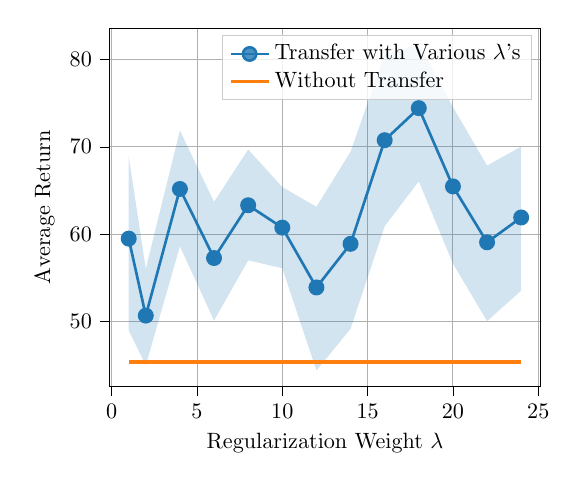
\begin{tikzpicture}[scale=0.8]

\definecolor{color0}{rgb}{0.12156862745098,0.466666666666667,0.705882352941177}
\definecolor{color1}{rgb}{1,0.498039215686275,0.0549019607843137}

\begin{axis}[
legend cell align={left},
legend style={fill opacity=0.8, draw opacity=1, text opacity=1, draw=white!80!black},
tick align=outside,
tick pos=left,
x grid style={white!69.0196078431373!black},
xmajorgrids,
xmin=-0.15, xmax=25.15,
xtick style={color=black},
xlabel={Regularization Weight $\lambda$},
y grid style={white!69.0196078431373!black},
ymajorgrids,
ymin=42.51114025, ymax=83.5967214166667,
ytick style={color=black},
ylabel={Average Return},
]
\path [fill=color0, fill opacity=0.2]
(axis cs:1,68.8835166666667)
--(axis cs:1,48.96444)
--(axis cs:2,44.9647116666667)
--(axis cs:4,58.59723)
--(axis cs:6,50.0959033333333)
--(axis cs:8,56.99296)
--(axis cs:10,56.087765)
--(axis cs:12,44.3786666666667)
--(axis cs:14,49.1427466666667)
--(axis cs:16,60.9039216666667)
--(axis cs:18,66.04868)
--(axis cs:20,56.6198883333333)
--(axis cs:22,50.0327633333333)
--(axis cs:24,53.5275133333333)
--(axis cs:24,70.0231633333333)
--(axis cs:24,70.0231633333333)
--(axis cs:22,67.85762)
--(axis cs:20,74.5615133333333)
--(axis cs:18,81.729195)
--(axis cs:16,80.5915783333333)
--(axis cs:14,69.4391683333333)
--(axis cs:12,63.1279883333333)
--(axis cs:10,65.3951133333333)
--(axis cs:8,69.693275)
--(axis cs:6,63.69618)
--(axis cs:4,71.870995)
--(axis cs:2,56.038055)
--(axis cs:1,68.8835166666667)
--cycle;

\addplot [very thick, color0, mark=*, mark size=3, mark options={solid}]
table {%
1 59.481312
2 50.6649345
4 65.1702346666667
6 57.2592315
8 63.306004
10 60.7404753333333
12 53.886415
14 58.8863686666667
16 70.7575176666667
18 74.4304055
20 65.4625285
22 59.0641981666667
24 61.9044141666667
};
\addlegendentry{Transfer with Various $\lambda$'s}
\addplot [ultra thick, color1]
table {%
1 45.334
2 45.334
4 45.334
6 45.334
8 45.334
10 45.334
12 45.334
14 45.334
16 45.334
18 45.334
20 45.334
22 45.334
24 45.334
};
\addlegendentry{Without Transfer}
\end{axis}

\end{tikzpicture}

    \vspace{-1em}
    \caption{In the Vec-to-pixel CartPole environment, under different selections of hyperparameter $\lambda$, the algorithm works better than learning from scratch (when $\lambda=0$). Results are averaged over 20 random seeds.}
    \label{fig:hyper}
    \vspace{-1em}
\end{wrapfigure}
\textbf{Hyper-parameter Test}\\
Figure~\ref{fig:hyper} further visualizes how the hyperparameter $\lambda$ (regularization weight) influences the transfer performance in the Vec-to-pixel CartPole environment. It can be found that the agent generally benefits from a larger $\lambda$, which suggests that the model-based regularization has a positive impact on the learning performance. For a wide range of $\lambda$'s, the agent always outperforms the learner without transfer (the learner with $\lambda=0$). Therefore, our algorithm is not sensitive to the hyperparameter $\lambda$, and a larger $\lambda$ is preferred to get better performance.
In Appendix~\ref{app:exp_drl}, we have provided the $\lambda$ selections for all experiments.
